% Options for packages loaded elsewhere
\PassOptionsToPackage{unicode}{hyperref}
\PassOptionsToPackage{hyphens}{url}
\PassOptionsToPackage{dvipsnames,svgnames,x11names}{xcolor}
%
\documentclass[
  letterpaper,
  DIV=11,
  numbers=noendperiod]{scrreprt}

\usepackage{amsmath,amssymb}
\usepackage{iftex}
\ifPDFTeX
  \usepackage[T1]{fontenc}
  \usepackage[utf8]{inputenc}
  \usepackage{textcomp} % provide euro and other symbols
\else % if luatex or xetex
  \usepackage{unicode-math}
  \defaultfontfeatures{Scale=MatchLowercase}
  \defaultfontfeatures[\rmfamily]{Ligatures=TeX,Scale=1}
\fi
\usepackage{lmodern}
\ifPDFTeX\else  
    % xetex/luatex font selection
\fi
% Use upquote if available, for straight quotes in verbatim environments
\IfFileExists{upquote.sty}{\usepackage{upquote}}{}
\IfFileExists{microtype.sty}{% use microtype if available
  \usepackage[]{microtype}
  \UseMicrotypeSet[protrusion]{basicmath} % disable protrusion for tt fonts
}{}
\makeatletter
\@ifundefined{KOMAClassName}{% if non-KOMA class
  \IfFileExists{parskip.sty}{%
    \usepackage{parskip}
  }{% else
    \setlength{\parindent}{0pt}
    \setlength{\parskip}{6pt plus 2pt minus 1pt}}
}{% if KOMA class
  \KOMAoptions{parskip=half}}
\makeatother
\usepackage{xcolor}
\setlength{\emergencystretch}{3em} % prevent overfull lines
\setcounter{secnumdepth}{5}
% Make \paragraph and \subparagraph free-standing
\ifx\paragraph\undefined\else
  \let\oldparagraph\paragraph
  \renewcommand{\paragraph}[1]{\oldparagraph{#1}\mbox{}}
\fi
\ifx\subparagraph\undefined\else
  \let\oldsubparagraph\subparagraph
  \renewcommand{\subparagraph}[1]{\oldsubparagraph{#1}\mbox{}}
\fi

\usepackage{color}
\usepackage{fancyvrb}
\newcommand{\VerbBar}{|}
\newcommand{\VERB}{\Verb[commandchars=\\\{\}]}
\DefineVerbatimEnvironment{Highlighting}{Verbatim}{commandchars=\\\{\}}
% Add ',fontsize=\small' for more characters per line
\usepackage{framed}
\definecolor{shadecolor}{RGB}{241,243,245}
\newenvironment{Shaded}{\begin{snugshade}}{\end{snugshade}}
\newcommand{\AlertTok}[1]{\textcolor[rgb]{0.68,0.00,0.00}{#1}}
\newcommand{\AnnotationTok}[1]{\textcolor[rgb]{0.37,0.37,0.37}{#1}}
\newcommand{\AttributeTok}[1]{\textcolor[rgb]{0.40,0.45,0.13}{#1}}
\newcommand{\BaseNTok}[1]{\textcolor[rgb]{0.68,0.00,0.00}{#1}}
\newcommand{\BuiltInTok}[1]{\textcolor[rgb]{0.00,0.23,0.31}{#1}}
\newcommand{\CharTok}[1]{\textcolor[rgb]{0.13,0.47,0.30}{#1}}
\newcommand{\CommentTok}[1]{\textcolor[rgb]{0.37,0.37,0.37}{#1}}
\newcommand{\CommentVarTok}[1]{\textcolor[rgb]{0.37,0.37,0.37}{\textit{#1}}}
\newcommand{\ConstantTok}[1]{\textcolor[rgb]{0.56,0.35,0.01}{#1}}
\newcommand{\ControlFlowTok}[1]{\textcolor[rgb]{0.00,0.23,0.31}{#1}}
\newcommand{\DataTypeTok}[1]{\textcolor[rgb]{0.68,0.00,0.00}{#1}}
\newcommand{\DecValTok}[1]{\textcolor[rgb]{0.68,0.00,0.00}{#1}}
\newcommand{\DocumentationTok}[1]{\textcolor[rgb]{0.37,0.37,0.37}{\textit{#1}}}
\newcommand{\ErrorTok}[1]{\textcolor[rgb]{0.68,0.00,0.00}{#1}}
\newcommand{\ExtensionTok}[1]{\textcolor[rgb]{0.00,0.23,0.31}{#1}}
\newcommand{\FloatTok}[1]{\textcolor[rgb]{0.68,0.00,0.00}{#1}}
\newcommand{\FunctionTok}[1]{\textcolor[rgb]{0.28,0.35,0.67}{#1}}
\newcommand{\ImportTok}[1]{\textcolor[rgb]{0.00,0.46,0.62}{#1}}
\newcommand{\InformationTok}[1]{\textcolor[rgb]{0.37,0.37,0.37}{#1}}
\newcommand{\KeywordTok}[1]{\textcolor[rgb]{0.00,0.23,0.31}{#1}}
\newcommand{\NormalTok}[1]{\textcolor[rgb]{0.00,0.23,0.31}{#1}}
\newcommand{\OperatorTok}[1]{\textcolor[rgb]{0.37,0.37,0.37}{#1}}
\newcommand{\OtherTok}[1]{\textcolor[rgb]{0.00,0.23,0.31}{#1}}
\newcommand{\PreprocessorTok}[1]{\textcolor[rgb]{0.68,0.00,0.00}{#1}}
\newcommand{\RegionMarkerTok}[1]{\textcolor[rgb]{0.00,0.23,0.31}{#1}}
\newcommand{\SpecialCharTok}[1]{\textcolor[rgb]{0.37,0.37,0.37}{#1}}
\newcommand{\SpecialStringTok}[1]{\textcolor[rgb]{0.13,0.47,0.30}{#1}}
\newcommand{\StringTok}[1]{\textcolor[rgb]{0.13,0.47,0.30}{#1}}
\newcommand{\VariableTok}[1]{\textcolor[rgb]{0.07,0.07,0.07}{#1}}
\newcommand{\VerbatimStringTok}[1]{\textcolor[rgb]{0.13,0.47,0.30}{#1}}
\newcommand{\WarningTok}[1]{\textcolor[rgb]{0.37,0.37,0.37}{\textit{#1}}}

\providecommand{\tightlist}{%
  \setlength{\itemsep}{0pt}\setlength{\parskip}{0pt}}\usepackage{longtable,booktabs,array}
\usepackage{calc} % for calculating minipage widths
% Correct order of tables after \paragraph or \subparagraph
\usepackage{etoolbox}
\makeatletter
\patchcmd\longtable{\par}{\if@noskipsec\mbox{}\fi\par}{}{}
\makeatother
% Allow footnotes in longtable head/foot
\IfFileExists{footnotehyper.sty}{\usepackage{footnotehyper}}{\usepackage{footnote}}
\makesavenoteenv{longtable}
\usepackage{graphicx}
\makeatletter
\def\maxwidth{\ifdim\Gin@nat@width>\linewidth\linewidth\else\Gin@nat@width\fi}
\def\maxheight{\ifdim\Gin@nat@height>\textheight\textheight\else\Gin@nat@height\fi}
\makeatother
% Scale images if necessary, so that they will not overflow the page
% margins by default, and it is still possible to overwrite the defaults
% using explicit options in \includegraphics[width, height, ...]{}
\setkeys{Gin}{width=\maxwidth,height=\maxheight,keepaspectratio}
% Set default figure placement to htbp
\makeatletter
\def\fps@figure{htbp}
\makeatother
% definitions for citeproc citations
\NewDocumentCommand\citeproctext{}{}
\NewDocumentCommand\citeproc{mm}{%
  \begingroup\def\citeproctext{#2}\cite{#1}\endgroup}
\makeatletter
 % allow citations to break across lines
 \let\@cite@ofmt\@firstofone
 % avoid brackets around text for \cite:
 \def\@biblabel#1{}
 \def\@cite#1#2{{#1\if@tempswa , #2\fi}}
\makeatother
\newlength{\cslhangindent}
\setlength{\cslhangindent}{1.5em}
\newlength{\csllabelwidth}
\setlength{\csllabelwidth}{3em}
\newenvironment{CSLReferences}[2] % #1 hanging-indent, #2 entry-spacing
 {\begin{list}{}{%
  \setlength{\itemindent}{0pt}
  \setlength{\leftmargin}{0pt}
  \setlength{\parsep}{0pt}
  % turn on hanging indent if param 1 is 1
  \ifodd #1
   \setlength{\leftmargin}{\cslhangindent}
   \setlength{\itemindent}{-1\cslhangindent}
  \fi
  % set entry spacing
  \setlength{\itemsep}{#2\baselineskip}}}
 {\end{list}}
\usepackage{calc}
\newcommand{\CSLBlock}[1]{\hfill\break\parbox[t]{\linewidth}{\strut\ignorespaces#1\strut}}
\newcommand{\CSLLeftMargin}[1]{\parbox[t]{\csllabelwidth}{\strut#1\strut}}
\newcommand{\CSLRightInline}[1]{\parbox[t]{\linewidth - \csllabelwidth}{\strut#1\strut}}
\newcommand{\CSLIndent}[1]{\hspace{\cslhangindent}#1}

\KOMAoption{captions}{tableheading}
\makeatletter
\@ifpackageloaded{bookmark}{}{\usepackage{bookmark}}
\makeatother
\makeatletter
\@ifpackageloaded{caption}{}{\usepackage{caption}}
\AtBeginDocument{%
\ifdefined\contentsname
  \renewcommand*\contentsname{Table of contents}
\else
  \newcommand\contentsname{Table of contents}
\fi
\ifdefined\listfigurename
  \renewcommand*\listfigurename{List of Figures}
\else
  \newcommand\listfigurename{List of Figures}
\fi
\ifdefined\listtablename
  \renewcommand*\listtablename{List of Tables}
\else
  \newcommand\listtablename{List of Tables}
\fi
\ifdefined\figurename
  \renewcommand*\figurename{Figure}
\else
  \newcommand\figurename{Figure}
\fi
\ifdefined\tablename
  \renewcommand*\tablename{Table}
\else
  \newcommand\tablename{Table}
\fi
}
\@ifpackageloaded{float}{}{\usepackage{float}}
\floatstyle{ruled}
\@ifundefined{c@chapter}{\newfloat{codelisting}{h}{lop}}{\newfloat{codelisting}{h}{lop}[chapter]}
\floatname{codelisting}{Listing}
\newcommand*\listoflistings{\listof{codelisting}{List of Listings}}
\makeatother
\makeatletter
\makeatother
\makeatletter
\@ifpackageloaded{caption}{}{\usepackage{caption}}
\@ifpackageloaded{subcaption}{}{\usepackage{subcaption}}
\makeatother
\ifLuaTeX
  \usepackage{selnolig}  % disable illegal ligatures
\fi
\usepackage{bookmark}

\IfFileExists{xurl.sty}{\usepackage{xurl}}{} % add URL line breaks if available
\urlstyle{same} % disable monospaced font for URLs
\hypersetup{
  pdftitle={Fake Accounts Instagram},
  pdfauthor={Antonio Cañete Baena},
  colorlinks=true,
  linkcolor={blue},
  filecolor={Maroon},
  citecolor={Blue},
  urlcolor={Blue},
  pdfcreator={LaTeX via pandoc}}

\title{Fake Accounts Instagram}
\author{Antonio Cañete Baena}
\date{Invalid Date}

\begin{document}
\maketitle

\renewcommand*\contentsname{Table of contents}
{
\hypersetup{linkcolor=}
\setcounter{tocdepth}{2}
\tableofcontents
}
\bookmarksetup{startatroot}

\chapter*{Introducción}\label{introducciuxf3n}
\addcontentsline{toc}{chapter}{Introducción}

\markboth{Introducción}{Introducción}

Este book recoge el proyecto realizado en la asignatura de
\emph{Laboratorio de computación científica} de la Universidad de
Málaga.

El objetivo de este proyecto es el análisis de un dataset de la
plataforma Kagle para extraer el maximo conocimiento posible usando las
técnicas vista durante la asignatura.

\bookmarksetup{startatroot}

\chapter*{1. DataSet:}\label{dataset}
\addcontentsline{toc}{chapter}{1. DataSet:}

\markboth{1. DataSet:}{1. DataSet:}

El dataSet que vamos a utilizar se llama '\textbf{Instagram fake spammer
genuine accounts',} obtenido de la web de kaggle. Este dataSet se
compone de diferentes cuentas de instgram tanto de spammers como de
usuarios genuinos.

Dicho dataSet esta formado por dos archivos, por un lado
\emph{test.csv,} un set de 120 entradas, 60 de cuentas genuinas y 60 de
cuentas de spammer. Y por otro lado, otro archivo \emph{train.csv},
formado por 576 entradas, donde al igual que en el archivo anterior, la
mitad son cuentas genuinas y la otra mitad son spammers.

\begin{description}
\item[Spammer]
El «\textbf{\emph{spam}}» es cualquier comunicación no solicitada
enviada en masa.El «\textbf{\emph{spamming}}» (que en español podría
traducirse como «espamear») es el acto de enviar estos mensajes. Y la
persona que envía los mensajes es un «\textbf{\emph{spammer}}».
\end{description}

\href{https://www.kaggle.com/datasets/free4ever1/instagram-fake-spammer-genuine-accounts}{Enlace
al DataSet}

\bookmarksetup{startatroot}

\chapter{Análisis exploratorio de
datos.}\label{anuxe1lisis-exploratorio-de-datos.}

El análisis exploratorio de datos consiste en analizar el conjunto o
conjuntos de datos de entrada con el objetivo de resumir sus
características principales ayudando a su comprensión para futuras
técnicas. Es una fase crucial en la ciencia de datos, ya que ayuda a los
analistas de datos a comprender mejor los datos antes de aplicar modelos
estadísticos más complejos o herramientas mas sofisticadas.

Para realizar dicho análisis, vamos a utilizar el \emph{meta-package} de
\texttt{tidyverse.}

\section{Carga de datos}\label{carga-de-datos}

Como hemos visto anteriormente, el dataSet contienen dos archivos con
datos, sin embargo, puesto que el archivo de \emph{train.csv} contiene
mas entradas de datos, vamos a utilizar dicho conjunto de datos para
aplicarle nuestras técnicas de análisis.

En primer lugar, vamos a cargar las librerias necesarias y los datos:

\begin{Shaded}
\begin{Highlighting}[]
\FunctionTok{library}\NormalTok{(tidyverse) }
\end{Highlighting}
\end{Shaded}

\begin{verbatim}
-- Attaching core tidyverse packages ------------------------ tidyverse 2.0.0 --
v dplyr     1.1.4     v readr     2.1.5
v forcats   1.0.0     v stringr   1.5.1
v ggplot2   3.5.0     v tibble    3.2.1
v lubridate 1.9.3     v tidyr     1.3.1
v purrr     1.0.2     
-- Conflicts ------------------------------------------ tidyverse_conflicts() --
x dplyr::filter() masks stats::filter()
x dplyr::lag()    masks stats::lag()
i Use the conflicted package (<http://conflicted.r-lib.org/>) to force all conflicts to become errors
\end{verbatim}

\begin{Shaded}
\begin{Highlighting}[]
\FunctionTok{library}\NormalTok{(readr) }
\NormalTok{datos }\OtherTok{\textless{}{-}} \FunctionTok{read\_csv}\NormalTok{(}\StringTok{"Data/train.csv"}\NormalTok{) }
\end{Highlighting}
\end{Shaded}

\begin{verbatim}
Rows: 576 Columns: 12
-- Column specification --------------------------------------------------------
Delimiter: ","
dbl (12): profile pic, nums/length username, fullname words, nums/length ful...

i Use `spec()` to retrieve the full column specification for this data.
i Specify the column types or set `show_col_types = FALSE` to quiet this message.
\end{verbatim}

Una vez tenemos nuestros datos, podemos ponernos manos a la obra.

Vamos a comenzar ojeando cuantas filas tenemos:

\begin{Shaded}
\begin{Highlighting}[]
\FunctionTok{nrow}\NormalTok{(datos)}
\end{Highlighting}
\end{Shaded}

\begin{verbatim}
[1] 576
\end{verbatim}

Y también vemos cuantos atributos tiene cada fila y sus nombres:

\begin{Shaded}
\begin{Highlighting}[]
\FunctionTok{ncol}\NormalTok{(datos)  }
\end{Highlighting}
\end{Shaded}

\begin{verbatim}
[1] 12
\end{verbatim}

\begin{Shaded}
\begin{Highlighting}[]
\FunctionTok{colnames}\NormalTok{(datos)}
\end{Highlighting}
\end{Shaded}

\begin{verbatim}
 [1] "profile pic"          "nums/length username" "fullname words"      
 [4] "nums/length fullname" "name==username"       "description length"  
 [7] "external URL"         "private"              "#posts"              
[10] "#followers"           "#follows"             "fake"                
\end{verbatim}

Veamos las primeras filas del dataset

\begin{Shaded}
\begin{Highlighting}[]
\FunctionTok{head}\NormalTok{(datos)}
\end{Highlighting}
\end{Shaded}

\begin{verbatim}
# A tibble: 6 x 12
  `profile pic` `nums/length username` `fullname words` `nums/length fullname`
          <dbl>                  <dbl>            <dbl>                  <dbl>
1             1                   0.27                0                      0
2             1                   0                   2                      0
3             1                   0.1                 2                      0
4             1                   0                   1                      0
5             1                   0                   2                      0
6             1                   0                   4                      0
# i 8 more variables: `name==username` <dbl>, `description length` <dbl>,
#   `external URL` <dbl>, private <dbl>, `#posts` <dbl>, `#followers` <dbl>,
#   `#follows` <dbl>, fake <dbl>
\end{verbatim}

Podemos ver que todas las columnas tienen valores numericos, pero vamos
a comprobarlo mirando dentro su estructura:

\begin{Shaded}
\begin{Highlighting}[]
\FunctionTok{str}\NormalTok{(datos)}
\end{Highlighting}
\end{Shaded}

\begin{verbatim}
spc_tbl_ [576 x 12] (S3: spec_tbl_df/tbl_df/tbl/data.frame)
 $ profile pic         : num [1:576] 1 1 1 1 1 1 1 1 1 1 ...
 $ nums/length username: num [1:576] 0.27 0 0.1 0 0 0 0 0 0 0 ...
 $ fullname words      : num [1:576] 0 2 2 1 2 4 2 2 0 2 ...
 $ nums/length fullname: num [1:576] 0 0 0 0 0 0 0 0 0 0 ...
 $ name==username      : num [1:576] 0 0 0 0 0 0 0 0 0 0 ...
 $ description length  : num [1:576] 53 44 0 82 0 81 50 0 71 40 ...
 $ external URL        : num [1:576] 0 0 0 0 0 1 0 0 0 1 ...
 $ private             : num [1:576] 0 0 1 0 1 0 0 0 0 0 ...
 $ #posts              : num [1:576] 32 286 13 679 6 344 16 33 72 213 ...
 $ #followers          : num [1:576] 1000 2740 159 414 151 ...
 $ #follows            : num [1:576] 955 533 98 651 126 ...
 $ fake                : num [1:576] 0 0 0 0 0 0 0 0 0 0 ...
 - attr(*, "spec")=
  .. cols(
  ..   `profile pic` = col_double(),
  ..   `nums/length username` = col_double(),
  ..   `fullname words` = col_double(),
  ..   `nums/length fullname` = col_double(),
  ..   `name==username` = col_double(),
  ..   `description length` = col_double(),
  ..   `external URL` = col_double(),
  ..   private = col_double(),
  ..   `#posts` = col_double(),
  ..   `#followers` = col_double(),
  ..   `#follows` = col_double(),
  ..   fake = col_double()
  .. )
 - attr(*, "problems")=<externalptr> 
\end{verbatim}

Hemos comprobado que todos los valores son del tipo numerico y double.

\begin{Shaded}
\begin{Highlighting}[]
\FunctionTok{anyNA}\NormalTok{(datos)}
\end{Highlighting}
\end{Shaded}

\begin{verbatim}
[1] FALSE
\end{verbatim}

Por ultimo comprobamos que no existen valores NA dentro del dataset, lo
que nos ayudara en su próximo análisis exploratorio.

\section{Analisis de atributos}\label{analisis-de-atributos}

Una vez visto un poco por encima la estructura del dataSet, vamos a
explorar uno a uno los atributos de cada fila, explorando su
significado, los valores limite, \ldots{}

\subsection{profile pic}\label{profile-pic}

Este es un atributo binario que indica si un usuario tiene foto de
perfil. Por lo tanto solo tenemos o 0 o 1.

\begin{Shaded}
\begin{Highlighting}[]
\FunctionTok{str}\NormalTok{(datos}\SpecialCharTok{$}\StringTok{\textasciigrave{}}\AttributeTok{profile pic}\StringTok{\textasciigrave{}}\NormalTok{)}
\end{Highlighting}
\end{Shaded}

\begin{verbatim}
 num [1:576] 1 1 1 1 1 1 1 1 1 1 ...
\end{verbatim}

\begin{Shaded}
\begin{Highlighting}[]
\FunctionTok{anyNA}\NormalTok{(datos}\SpecialCharTok{$}\StringTok{\textasciigrave{}}\AttributeTok{profile pic}\StringTok{\textasciigrave{}}\NormalTok{)}
\end{Highlighting}
\end{Shaded}

\begin{verbatim}
[1] FALSE
\end{verbatim}

Vemos que esta columna no contiene ningun NA.

Vamos a visualizar la proporcion de usuarios con foto de perfil:

\begin{Shaded}
\begin{Highlighting}[]
\FunctionTok{hist}\NormalTok{(datos}\SpecialCharTok{$}\StringTok{\textasciigrave{}}\AttributeTok{profile pic}\StringTok{\textasciigrave{}}\NormalTok{, }\AttributeTok{breaks =} \DecValTok{2}\NormalTok{, }\AttributeTok{main=}\StringTok{"Fotos de perfil"}\NormalTok{ )}
\end{Highlighting}
\end{Shaded}

\includegraphics{analisisExploratorio_files/figure-pdf/unnamed-chunk-9-1.pdf}

Observamos que más de la mitad de los usuarios tienen foto de perfil.

\subsection{nums/length username}\label{numslength-username}

Este atributo representa el ratio de numero de caracteres numericos en
el nombre de usuario respecto su longutud. Ej: Ant234 -\textgreater{}
Ratio 1.

\begin{Shaded}
\begin{Highlighting}[]
\FunctionTok{hist}\NormalTok{(datos}\SpecialCharTok{$}\StringTok{\textasciigrave{}}\AttributeTok{nums/length username}\StringTok{\textasciigrave{}}\NormalTok{, }\AttributeTok{main=}\StringTok{"Ratio caracteres num en usuario"}\NormalTok{ )}
\end{Highlighting}
\end{Shaded}

\includegraphics{analisisExploratorio_files/figure-pdf/unnamed-chunk-10-1.pdf}

\subsection{fullname words}\label{fullname-words}

Este atributo representa la cantidad de palabras que componen el nombre
del usuario.

\begin{Shaded}
\begin{Highlighting}[]
\FunctionTok{max}\NormalTok{(datos}\SpecialCharTok{$}\StringTok{\textasciigrave{}}\AttributeTok{fullname words}\StringTok{\textasciigrave{}}\NormalTok{)}
\end{Highlighting}
\end{Shaded}

\begin{verbatim}
[1] 12
\end{verbatim}

Observamos que hay uno o varios usuarios cuyo nombre tiene 12 palabras
de longitud, algo que es poco común.

\begin{Shaded}
\begin{Highlighting}[]
\FunctionTok{hist}\NormalTok{(datos}\SpecialCharTok{$}\StringTok{\textasciigrave{}}\AttributeTok{fullname words}\StringTok{\textasciigrave{}}\NormalTok{, }\AttributeTok{main=}\StringTok{"Num palabra nombre"}\NormalTok{ )}
\end{Highlighting}
\end{Shaded}

\includegraphics{analisisExploratorio_files/figure-pdf/unnamed-chunk-12-1.pdf}

Analizando el histograma, vemos que la mayoría de usuarios tiene entre 0
y 1 palabras en su nombre.

\begin{Shaded}
\begin{Highlighting}[]
\FunctionTok{count}\NormalTok{(}\FunctionTok{filter}\NormalTok{(datos,}\StringTok{\textasciigrave{}}\AttributeTok{fullname words}\StringTok{\textasciigrave{}}\SpecialCharTok{==}\DecValTok{1} \SpecialCharTok{|} \StringTok{\textasciigrave{}}\AttributeTok{fullname words}\StringTok{\textasciigrave{}}\SpecialCharTok{==}\DecValTok{2}\NormalTok{))}\SpecialCharTok{/}\FunctionTok{count}\NormalTok{(datos)}\SpecialCharTok{*}\DecValTok{100}
\end{Highlighting}
\end{Shaded}

\begin{verbatim}
         n
1 81.59722
\end{verbatim}

En concreto el 81,6\% de los datos tienen entre 0 y 1 palabras en su
nombre.

\subsection{nums/length fullname}\label{numslength-fullname}

Este atributo representa el ratio de numero de caracteres numéricos en
el nombre completo del usuario respecto su longitud.

\begin{Shaded}
\begin{Highlighting}[]
\FunctionTok{hist}\NormalTok{(datos}\SpecialCharTok{$}\StringTok{\textasciigrave{}}\AttributeTok{nums/length fullname}\StringTok{\textasciigrave{}}\NormalTok{, }\AttributeTok{main=}\StringTok{"Ratio caracteres num en nombre"}\NormalTok{ )}
\end{Highlighting}
\end{Shaded}

\includegraphics{analisisExploratorio_files/figure-pdf/unnamed-chunk-14-1.pdf}

Observamos que es bastante inusual que un usuario tenga caracteres en su
nombre completo, mientra que, como hemos visto antes, en el nombre de
usuario, es más frecuente encontrar caracteres.

\subsection{name==username}\label{nameusername}

Este atributo es un atributo binario que representa si el usuario tiene
el mismo nombre de usuario y nombre completo.

\begin{Shaded}
\begin{Highlighting}[]
\FunctionTok{hist}\NormalTok{(datos}\SpecialCharTok{$}\StringTok{\textasciigrave{}}\AttributeTok{name==username}\StringTok{\textasciigrave{}}\NormalTok{, }\AttributeTok{breaks =} \DecValTok{2}\NormalTok{, }\AttributeTok{main=}\StringTok{"Nombre igual a usuario"}\NormalTok{ )}
\end{Highlighting}
\end{Shaded}

\includegraphics{analisisExploratorio_files/figure-pdf/unnamed-chunk-15-1.pdf}

Concluimos que el bastante inusual que un usuarios tenga el mismo nombre
de usuario y nombre completo.

\subsection{description length}\label{description-length}

Este atributo representa la longitud de la descripción del perfil de
usuario (en caracteres).

\begin{Shaded}
\begin{Highlighting}[]
\FunctionTok{hist}\NormalTok{(datos}\SpecialCharTok{$}\StringTok{\textasciigrave{}}\AttributeTok{description length}\StringTok{\textasciigrave{}}\NormalTok{, }\AttributeTok{main=}\StringTok{"Num carateres de la descripcion"}\NormalTok{ )}
\end{Highlighting}
\end{Shaded}

\includegraphics{analisisExploratorio_files/figure-pdf/unnamed-chunk-16-1.pdf}

Podemos intuir que el máximo de caracteres que ofrece Instagram en su
descripción es 150, cuyo limite es alcanzado por pocos usuarios del
DataSet:

\begin{Shaded}
\begin{Highlighting}[]
\FunctionTok{filter}\NormalTok{(datos,datos}\SpecialCharTok{$}\StringTok{\textasciigrave{}}\AttributeTok{description length}\StringTok{\textasciigrave{}} \SpecialCharTok{==}\DecValTok{150}\NormalTok{) }\SpecialCharTok{\%\textgreater{}\%} \FunctionTok{count}\NormalTok{() }\SpecialCharTok{\%\textgreater{}\%} \FunctionTok{summarise}\NormalTok{(}\StringTok{\textasciigrave{}}\AttributeTok{Num de usuarios}\StringTok{\textasciigrave{}}\OtherTok{=}\NormalTok{n)}
\end{Highlighting}
\end{Shaded}

\begin{verbatim}
# A tibble: 1 x 1
  `Num de usuarios`
              <int>
1                 2
\end{verbatim}

Viendo el histograma, descubrimos que la mayoría de usuarios tienen una
descripción con pocos caracteres, pero vamos a calcular la media para
poder tener una idea:

\begin{Shaded}
\begin{Highlighting}[]
\FunctionTok{mean}\NormalTok{(datos}\SpecialCharTok{$}\StringTok{\textasciigrave{}}\AttributeTok{description length}\StringTok{\textasciigrave{}}\NormalTok{)}
\end{Highlighting}
\end{Shaded}

\begin{verbatim}
[1] 22.62326
\end{verbatim}

Encontramos que la media de caracteres en la descripción, lo que,
dependiendo del idioma, puede ser una pequeña frase o algunas palabras.
Las descripciones largar son menos frecuentes.

\subsection{external URL}\label{external-url}

Este atributo es un atributo binario que representa si el perfil tiene
algún enlaza externo en el.

\begin{Shaded}
\begin{Highlighting}[]
\FunctionTok{hist}\NormalTok{(datos}\SpecialCharTok{$}\StringTok{\textasciigrave{}}\AttributeTok{external URL}\StringTok{\textasciigrave{}}\NormalTok{, }\AttributeTok{breaks =} \DecValTok{2}\NormalTok{, }\AttributeTok{main=}\StringTok{"Enlace en el perfil?"}\NormalTok{ )}
\end{Highlighting}
\end{Shaded}

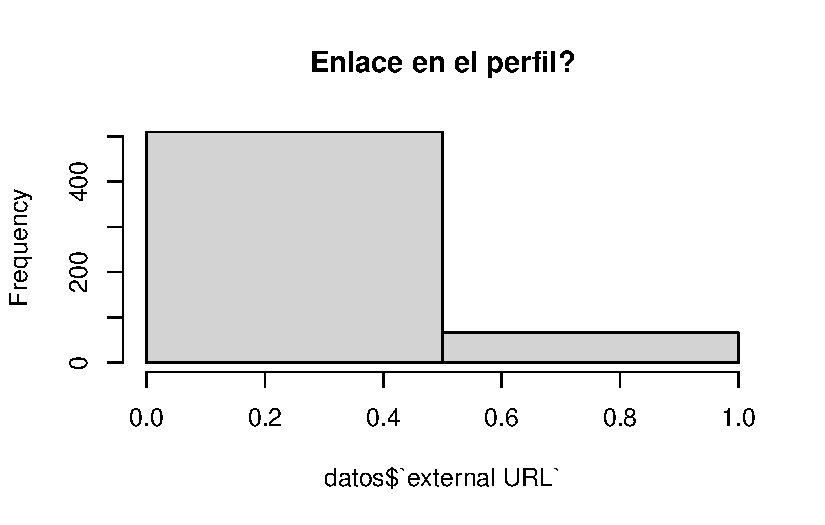
\includegraphics{analisisExploratorio_files/figure-pdf/unnamed-chunk-19-1.pdf}

Lo mas común son los perfiles sin enlaces externos.

\subsection{private}\label{private}

Este atributo es un atributo binario que representa si el perfil es
privado o publico.

\begin{Shaded}
\begin{Highlighting}[]
\FunctionTok{hist}\NormalTok{(datos}\SpecialCharTok{$}\StringTok{\textasciigrave{}}\AttributeTok{private}\StringTok{\textasciigrave{}}\NormalTok{, }\AttributeTok{breaks =} \DecValTok{2}\NormalTok{, }\AttributeTok{main=}\StringTok{"Perfil privado?"}\NormalTok{ )}
\end{Highlighting}
\end{Shaded}

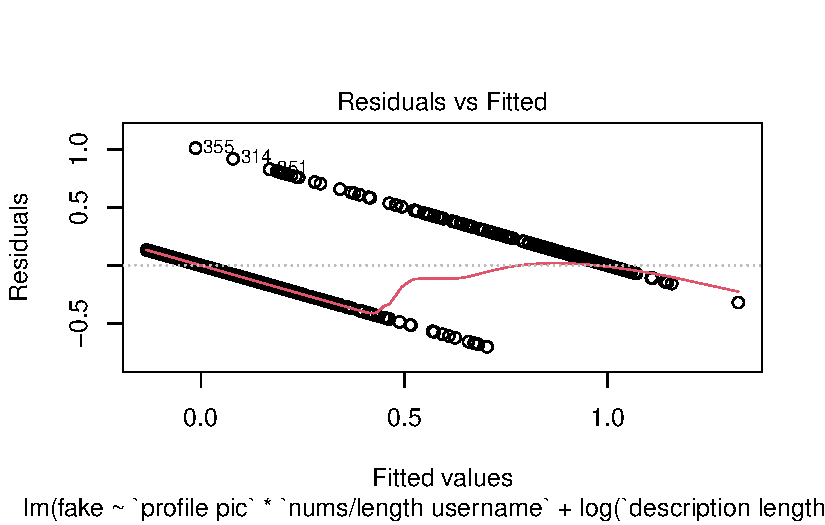
\includegraphics{analisisExploratorio_files/figure-pdf/unnamed-chunk-20-1.pdf}

En este atributo encontramos algo mas de igualdad, el numero de cuentas
privadas son poco mas de la mitad del numero de publicas:

\begin{Shaded}
\begin{Highlighting}[]
\NormalTok{datos }\SpecialCharTok{\%\textgreater{}\%} \FunctionTok{mutate}\NormalTok{(}\AttributeTok{private =} \FunctionTok{ifelse}\NormalTok{(private}\SpecialCharTok{==}\DecValTok{1}\NormalTok{,}\StringTok{"Privada"}\NormalTok{,}\StringTok{"Publica"}\NormalTok{)) }\SpecialCharTok{\%\textgreater{}\%}  \FunctionTok{group\_by}\NormalTok{(private) }\SpecialCharTok{\%\textgreater{}\%} \FunctionTok{count}\NormalTok{() }\SpecialCharTok{\%\textgreater{}\%}  \FunctionTok{summarise}\NormalTok{(}\AttributeTok{Numero =} \FunctionTok{sum}\NormalTok{(n))  }
\end{Highlighting}
\end{Shaded}

\begin{verbatim}
# A tibble: 2 x 2
  private Numero
  <chr>    <int>
1 Privada    220
2 Publica    356
\end{verbatim}

\subsection{post}\label{post}

Este atributo representa el numero de publicaciones de la cuenta.

\begin{Shaded}
\begin{Highlighting}[]
\FunctionTok{hist}\NormalTok{(datos}\SpecialCharTok{$}\StringTok{\textasciigrave{}}\AttributeTok{\#posts}\StringTok{\textasciigrave{}}\NormalTok{,  }\AttributeTok{main=}\StringTok{"Fotos de perfil"}\NormalTok{ )}
\end{Highlighting}
\end{Shaded}

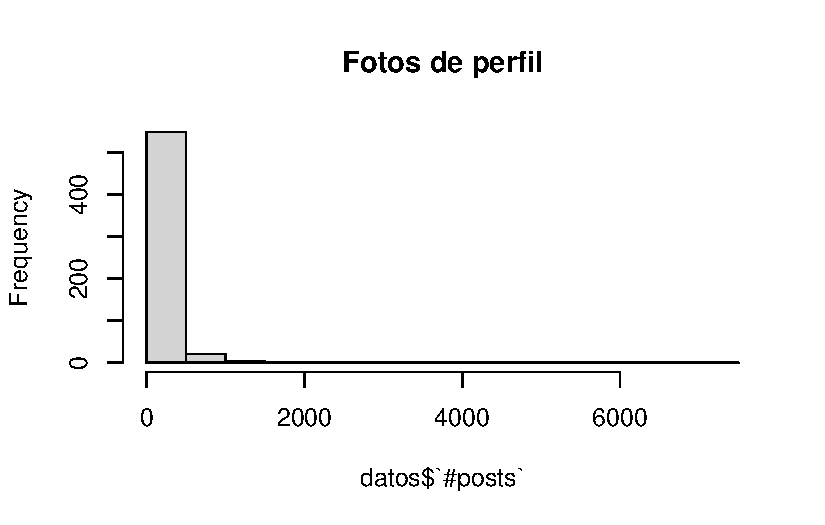
\includegraphics{analisisExploratorio_files/figure-pdf/unnamed-chunk-22-1.pdf}

\begin{Shaded}
\begin{Highlighting}[]
\FunctionTok{max}\NormalTok{(datos}\SpecialCharTok{$}\StringTok{\textasciigrave{}}\AttributeTok{\#posts}\StringTok{\textasciigrave{}}\NormalTok{)}
\end{Highlighting}
\end{Shaded}

\begin{verbatim}
[1] 7389
\end{verbatim}

Obtenemos un histograma un poco extrano al haber algun valor muy alto de
publicaciones, vamos a buscarlo:

\begin{Shaded}
\begin{Highlighting}[]
\FunctionTok{max}\NormalTok{(datos}\SpecialCharTok{$}\StringTok{\textasciigrave{}}\AttributeTok{\#posts}\StringTok{\textasciigrave{}}\NormalTok{)}
\end{Highlighting}
\end{Shaded}

\begin{verbatim}
[1] 7389
\end{verbatim}

Vemos que es un valor bastante raro o que se podría tratar de alguna
cuenta que publicase mucho contenido a diario. Vamos a verla:

\begin{Shaded}
\begin{Highlighting}[]
\NormalTok{datos }\SpecialCharTok{\%\textgreater{}\%} \FunctionTok{filter}\NormalTok{(}\StringTok{\textasciigrave{}}\AttributeTok{\#posts}\StringTok{\textasciigrave{}}\SpecialCharTok{==}\DecValTok{7389}\NormalTok{)}
\end{Highlighting}
\end{Shaded}

\begin{verbatim}
# A tibble: 1 x 12
  `profile pic` `nums/length username` `fullname words` `nums/length fullname`
          <dbl>                  <dbl>            <dbl>                  <dbl>
1             1                      0                0                      0
# i 8 more variables: `name==username` <dbl>, `description length` <dbl>,
#   `external URL` <dbl>, private <dbl>, `#posts` <dbl>, `#followers` <dbl>,
#   `#follows` <dbl>, fake <dbl>
\end{verbatim}

Como dato, la cuenta de Dwayne Johnson, ex-luchador de la WWE y exitoso
actor de Hollywood, tiene unos 7800 post, por lo que dicho valor puede
ser debido a la cuenta de algún famoso.

Vamos a volver a dibujar el histograma pero con un umbral un poco mas
razonable:

\begin{Shaded}
\begin{Highlighting}[]
\NormalTok{post\_filtrados }\OtherTok{\textless{}{-}}\NormalTok{ datos }\SpecialCharTok{\%\textgreater{}\%} \FunctionTok{select}\NormalTok{(}\StringTok{\textasciigrave{}}\AttributeTok{\#posts}\StringTok{\textasciigrave{}}\NormalTok{)}\SpecialCharTok{\%\textgreater{}\%} \FunctionTok{filter}\NormalTok{(}\StringTok{\textasciigrave{}}\AttributeTok{\#posts}\StringTok{\textasciigrave{}} \SpecialCharTok{\textless{}}\DecValTok{500}\NormalTok{)}
\FunctionTok{hist}\NormalTok{(post\_filtrados}\SpecialCharTok{$}\StringTok{\textasciigrave{}}\AttributeTok{\#posts}\StringTok{\textasciigrave{}}\NormalTok{)}
\end{Highlighting}
\end{Shaded}

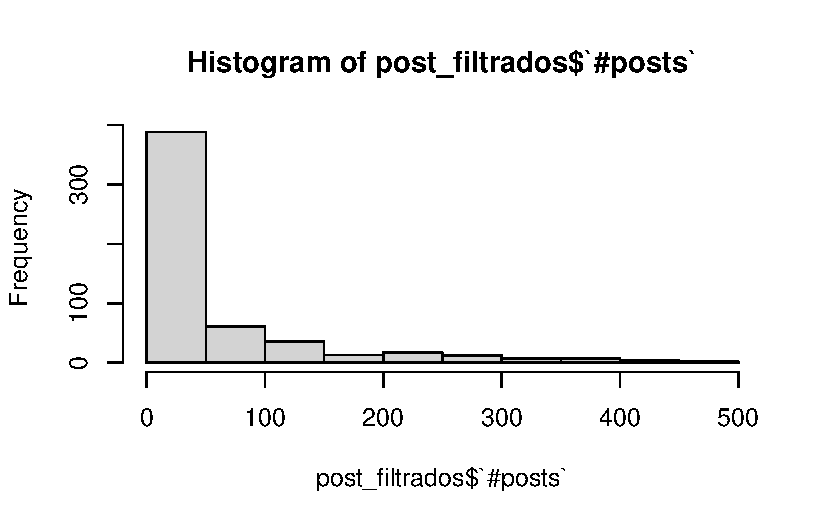
\includegraphics{analisisExploratorio_files/figure-pdf/unnamed-chunk-25-1.pdf}

Ahora ya podemos extraer informacion mas facilmente, como que la mayoria
de usuarios tiene menos de 50 publicaciones, vamos a verlo en mas
detalle:

\begin{Shaded}
\begin{Highlighting}[]
\NormalTok{post\_filtrados }\OtherTok{\textless{}{-}}\NormalTok{ datos }\SpecialCharTok{\%\textgreater{}\%} \FunctionTok{select}\NormalTok{(}\StringTok{\textasciigrave{}}\AttributeTok{\#posts}\StringTok{\textasciigrave{}}\NormalTok{)}\SpecialCharTok{\%\textgreater{}\%} \FunctionTok{filter}\NormalTok{(}\StringTok{\textasciigrave{}}\AttributeTok{\#posts}\StringTok{\textasciigrave{}} \SpecialCharTok{\textless{}}\DecValTok{50}\NormalTok{)}
\FunctionTok{hist}\NormalTok{(post\_filtrados}\SpecialCharTok{$}\StringTok{\textasciigrave{}}\AttributeTok{\#posts}\StringTok{\textasciigrave{}}\NormalTok{)}
\end{Highlighting}
\end{Shaded}

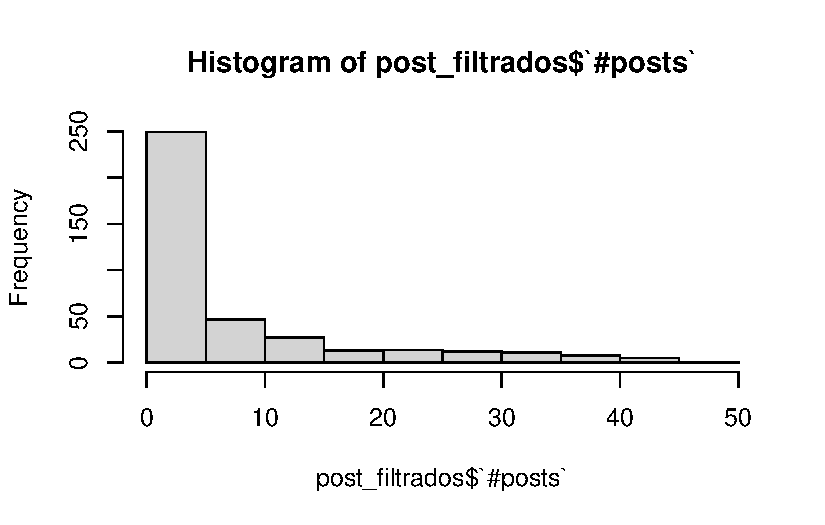
\includegraphics{analisisExploratorio_files/figure-pdf/unnamed-chunk-26-1.pdf}

Observamos que hay un gran numero de usuarios con menos de 5 posts.
Vamos a ver cuantos de ellos tiene 0 posts y a ver la media total:

\begin{Shaded}
\begin{Highlighting}[]
\NormalTok{datos }\SpecialCharTok{\%\textgreater{}\%} \FunctionTok{filter}\NormalTok{(}\StringTok{\textasciigrave{}}\AttributeTok{\#posts}\StringTok{\textasciigrave{}}\SpecialCharTok{==}\DecValTok{0}\NormalTok{) }\SpecialCharTok{\%\textgreater{}\%} \FunctionTok{count}\NormalTok{()}
\end{Highlighting}
\end{Shaded}

\begin{verbatim}
# A tibble: 1 x 1
      n
  <int>
1   157
\end{verbatim}

\begin{Shaded}
\begin{Highlighting}[]
\FunctionTok{mean}\NormalTok{(datos}\SpecialCharTok{$}\StringTok{\textasciigrave{}}\AttributeTok{\#posts}\StringTok{\textasciigrave{}}\NormalTok{)}
\end{Highlighting}
\end{Shaded}

\begin{verbatim}
[1] 107.4896
\end{verbatim}

Aunque como antes hemos visto que hay usuarios con un gran numero de
posts, esta media puede ser no muy significativa.

Vamos a analizar entonces sus cuartiles y mediana:

\begin{Shaded}
\begin{Highlighting}[]
\FunctionTok{summary}\NormalTok{(datos}\SpecialCharTok{$}\StringTok{\textasciigrave{}}\AttributeTok{\#posts}\StringTok{\textasciigrave{}}\NormalTok{)}
\end{Highlighting}
\end{Shaded}

\begin{verbatim}
   Min. 1st Qu.  Median    Mean 3rd Qu.    Max. 
    0.0     0.0     9.0   107.5    81.5  7389.0 
\end{verbatim}

\subsection{followers}\label{followers}

Este atributo representa el numero de seguidores de la cuenta.

\begin{Shaded}
\begin{Highlighting}[]
\FunctionTok{hist}\NormalTok{(datos}\SpecialCharTok{$}\StringTok{\textasciigrave{}}\AttributeTok{\#followers}\StringTok{\textasciigrave{}}\NormalTok{, }\AttributeTok{main=}\StringTok{"Numero de seguidores"}\NormalTok{ )}
\end{Highlighting}
\end{Shaded}

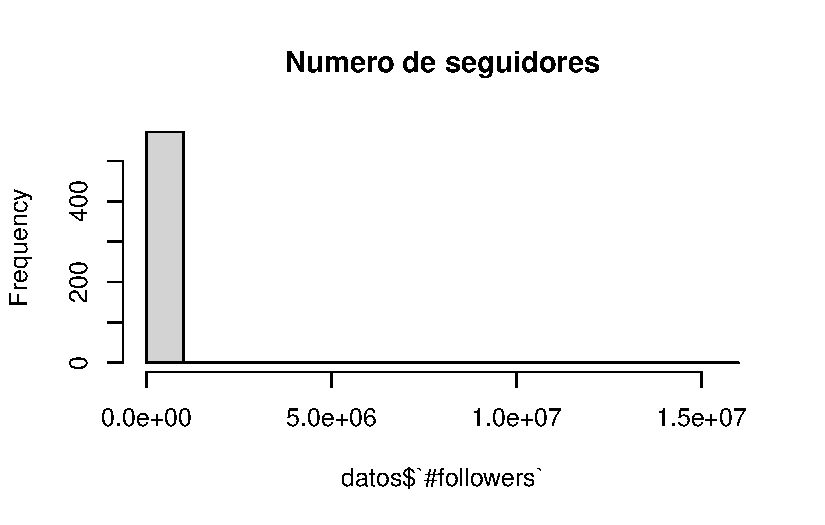
\includegraphics{analisisExploratorio_files/figure-pdf/unnamed-chunk-29-1.pdf}

\begin{Shaded}
\begin{Highlighting}[]
\FunctionTok{max}\NormalTok{(datos}\SpecialCharTok{$}\StringTok{\textasciigrave{}}\AttributeTok{\#followers}\StringTok{\textasciigrave{}}\NormalTok{)}
\end{Highlighting}
\end{Shaded}

\begin{verbatim}
[1] 15338538
\end{verbatim}

Como en el atributo anteriro, este histograma no tiene sentido porque
hay algun valor muy alto

\begin{Shaded}
\begin{Highlighting}[]
\FunctionTok{max}\NormalTok{(datos}\SpecialCharTok{$}\StringTok{\textasciigrave{}}\AttributeTok{\#followers}\StringTok{\textasciigrave{}}\NormalTok{)}
\end{Highlighting}
\end{Shaded}

\begin{verbatim}
[1] 15338538
\end{verbatim}

Dicho valor solo tiene sentido que sea debido a una cuenta de alguna
celebridad, vamos a comprobar si es el mismo que tiene similitud con el
valor anómalo de post encontrado anteriormente:

\begin{Shaded}
\begin{Highlighting}[]
\NormalTok{datos }\SpecialCharTok{\%\textgreater{}\%} \FunctionTok{filter}\NormalTok{ (}\StringTok{\textasciigrave{}}\AttributeTok{\#followers}\StringTok{\textasciigrave{}}\SpecialCharTok{==}\FunctionTok{max}\NormalTok{(}\StringTok{\textasciigrave{}}\AttributeTok{\#followers}\StringTok{\textasciigrave{}}\NormalTok{)) }\SpecialCharTok{\%\textgreater{}\%} \FunctionTok{select}\NormalTok{(}\StringTok{\textasciigrave{}}\AttributeTok{\#posts}\StringTok{\textasciigrave{}}\NormalTok{)}
\end{Highlighting}
\end{Shaded}

\begin{verbatim}
# A tibble: 1 x 1
  `#posts`
     <dbl>
1      148
\end{verbatim}

Aun pudiendo ser la cuenta de una celebridad, vemos que tiene un numero
de post relativamente normal, comparado con el valor de 7389 post que
obtuvimos anteriormente.

Vamos a volver a hacer el histograma con un nuevo umbral mas bajo:

\begin{Shaded}
\begin{Highlighting}[]
\NormalTok{followers\_filtrados }\OtherTok{\textless{}{-}}\NormalTok{ datos }\SpecialCharTok{\%\textgreater{}\%} \FunctionTok{select}\NormalTok{(}\StringTok{\textasciigrave{}}\AttributeTok{\#followers}\StringTok{\textasciigrave{}}\NormalTok{)}\SpecialCharTok{\%\textgreater{}\%} \FunctionTok{filter}\NormalTok{(}\StringTok{\textasciigrave{}}\AttributeTok{\#followers}\StringTok{\textasciigrave{}} \SpecialCharTok{\textless{}}\DecValTok{1000}\NormalTok{)}
\FunctionTok{hist}\NormalTok{(followers\_filtrados}\SpecialCharTok{$}\StringTok{\textasciigrave{}}\AttributeTok{\#followers}\StringTok{\textasciigrave{}}\NormalTok{)}
\end{Highlighting}
\end{Shaded}

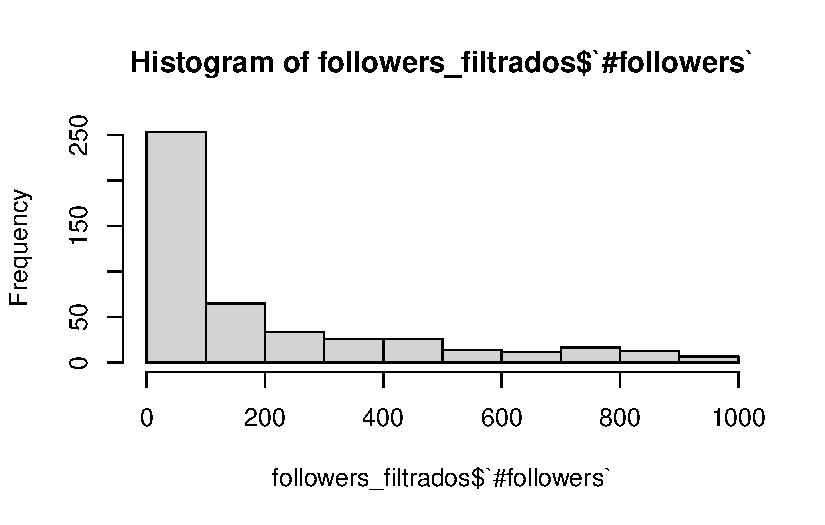
\includegraphics{analisisExploratorio_files/figure-pdf/unnamed-chunk-32-1.pdf}

Observamos que la mayoría de usuarios no tiene gran numero de
seguidores, en concreto, menos de 100.

Vamos a verlo

\begin{Shaded}
\begin{Highlighting}[]
\NormalTok{followers\_filtrados }\OtherTok{\textless{}{-}}\NormalTok{ datos }\SpecialCharTok{\%\textgreater{}\%} \FunctionTok{select}\NormalTok{(}\StringTok{\textasciigrave{}}\AttributeTok{\#followers}\StringTok{\textasciigrave{}}\NormalTok{)}\SpecialCharTok{\%\textgreater{}\%} \FunctionTok{filter}\NormalTok{(}\StringTok{\textasciigrave{}}\AttributeTok{\#followers}\StringTok{\textasciigrave{}} \SpecialCharTok{\textless{}}\DecValTok{100}\NormalTok{)}
\FunctionTok{hist}\NormalTok{(followers\_filtrados}\SpecialCharTok{$}\StringTok{\textasciigrave{}}\AttributeTok{\#followers}\StringTok{\textasciigrave{}}\NormalTok{)}
\end{Highlighting}
\end{Shaded}

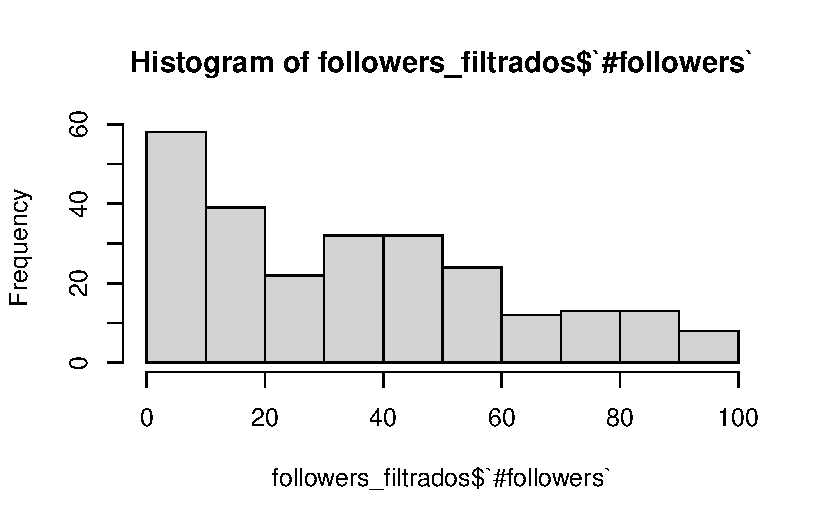
\includegraphics{analisisExploratorio_files/figure-pdf/unnamed-chunk-33-1.pdf}

Vemos que en este intervalo, si esta mas repartidas las frecuencias.
Aunque resulta curioso que una gran cantidad de usuarios no llegue a los
50 seguidores.

Viendo que hay algunos usuarios con un gran numero de seguidores, no
tiene sentido tomar el valor de la mediana como referencia ya que esta
no es significativa en este caso, por lo que vamos a analizar los
cuartiles y la mediana en su lugar.

\begin{Shaded}
\begin{Highlighting}[]
\FunctionTok{mean}\NormalTok{(datos}\SpecialCharTok{$}\StringTok{\textasciigrave{}}\AttributeTok{\#followers}\StringTok{\textasciigrave{}}\NormalTok{)}
\end{Highlighting}
\end{Shaded}

\begin{verbatim}
[1] 85307.24
\end{verbatim}

\begin{Shaded}
\begin{Highlighting}[]
\FunctionTok{summary}\NormalTok{(datos}\SpecialCharTok{$}\StringTok{\textasciigrave{}}\AttributeTok{\#followers}\StringTok{\textasciigrave{}}\NormalTok{)}
\end{Highlighting}
\end{Shaded}

\begin{verbatim}
    Min.  1st Qu.   Median     Mean  3rd Qu.     Max. 
       0       39      150    85307      716 15338538 
\end{verbatim}

Sabiendo que la mediana divide al 50\% de los datos, dicho valor es mas
significativo que la media.

\subsection{follows}\label{follows}

Este atributo representa el numero de usuarios seguidos por la cuenta.

\begin{Shaded}
\begin{Highlighting}[]
\FunctionTok{hist}\NormalTok{(datos}\SpecialCharTok{$}\StringTok{\textasciigrave{}}\AttributeTok{\#follows}\StringTok{\textasciigrave{}}\NormalTok{, }\AttributeTok{main=}\StringTok{"Numero de seguidos"}\NormalTok{ )}
\end{Highlighting}
\end{Shaded}

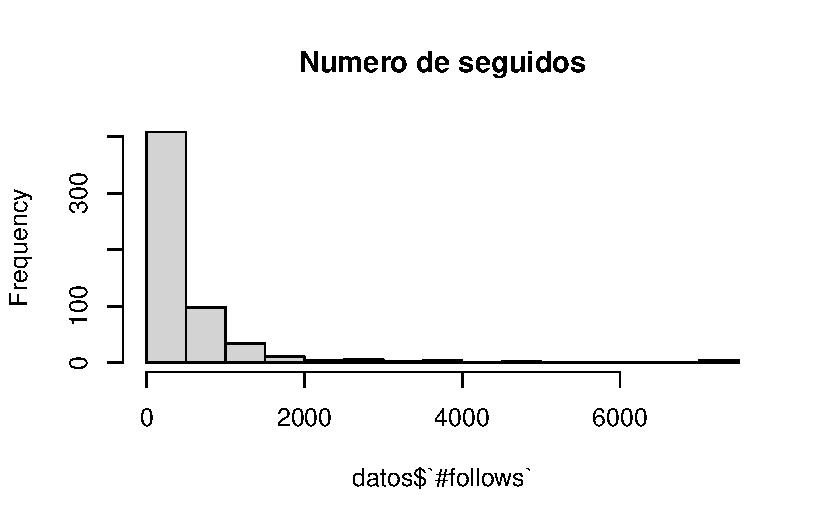
\includegraphics{analisisExploratorio_files/figure-pdf/unnamed-chunk-35-1.pdf}

\begin{Shaded}
\begin{Highlighting}[]
\FunctionTok{max}\NormalTok{(datos}\SpecialCharTok{$}\StringTok{\textasciigrave{}}\AttributeTok{\#follows}\StringTok{\textasciigrave{}}\NormalTok{)}
\end{Highlighting}
\end{Shaded}

\begin{verbatim}
[1] 7500
\end{verbatim}

Al igual que en los dos anteriores, los valores máximos hacen que
nuestro histograma no sea muy entendible, vamos a estudiarlo:

\begin{Shaded}
\begin{Highlighting}[]
\FunctionTok{max}\NormalTok{(datos}\SpecialCharTok{$}\StringTok{\textasciigrave{}}\AttributeTok{\#follows}\StringTok{\textasciigrave{}}\NormalTok{)}
\end{Highlighting}
\end{Shaded}

\begin{verbatim}
[1] 7500
\end{verbatim}

Dicho valor corresponde con el valor máximo de cuentas que Instagram
permite a los usuarios seguir para reducir el spam. Por lo tanto, las
cuentas que siguen a un gran numero de personas se pueden llegar a
asociar a spammers. Vamos a ver cuantas cuentas están en este limite:

\begin{Shaded}
\begin{Highlighting}[]
\FunctionTok{count}\NormalTok{(}\FunctionTok{filter}\NormalTok{(datos,datos}\SpecialCharTok{$}\StringTok{\textasciigrave{}}\AttributeTok{\#follows}\StringTok{\textasciigrave{}}\SpecialCharTok{==}\DecValTok{7500}\NormalTok{))}
\end{Highlighting}
\end{Shaded}

\begin{verbatim}
# A tibble: 1 x 1
      n
  <int>
1     2
\end{verbatim}

Ahora para poder ahcernos una mejor idea vamos a volver a dibujar el
histograma con un nuevo umbral reducido.

\begin{Shaded}
\begin{Highlighting}[]
\NormalTok{follows\_filtrados }\OtherTok{\textless{}{-}}\NormalTok{ datos }\SpecialCharTok{\%\textgreater{}\%} \FunctionTok{select}\NormalTok{(}\StringTok{\textasciigrave{}}\AttributeTok{\#follows}\StringTok{\textasciigrave{}}\NormalTok{)}\SpecialCharTok{\%\textgreater{}\%} \FunctionTok{filter}\NormalTok{(}\StringTok{\textasciigrave{}}\AttributeTok{\#follows}\StringTok{\textasciigrave{}} \SpecialCharTok{\textless{}}\DecValTok{1000}\NormalTok{)}
\FunctionTok{hist}\NormalTok{(follows\_filtrados}\SpecialCharTok{$}\StringTok{\textasciigrave{}}\AttributeTok{\#follows}\StringTok{\textasciigrave{}}\NormalTok{)}
\end{Highlighting}
\end{Shaded}

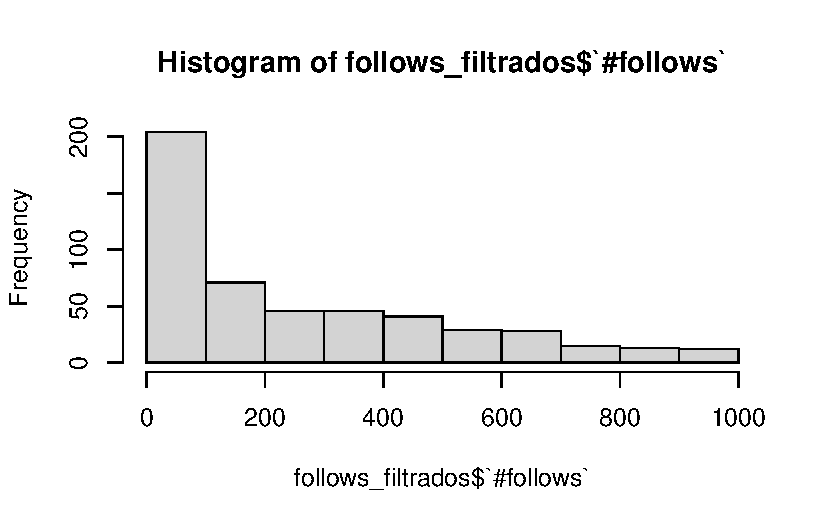
\includegraphics{analisisExploratorio_files/figure-pdf/unnamed-chunk-38-1.pdf}

Observamos que mas de la mitad de usuarios no sigue a muchas otras
cuentas, en concreto, menos de 100.

Vamos a verlo:

\begin{Shaded}
\begin{Highlighting}[]
\NormalTok{follows\_filtrados }\OtherTok{\textless{}{-}}\NormalTok{ datos }\SpecialCharTok{\%\textgreater{}\%} \FunctionTok{select}\NormalTok{(}\StringTok{\textasciigrave{}}\AttributeTok{\#follows}\StringTok{\textasciigrave{}}\NormalTok{)}\SpecialCharTok{\%\textgreater{}\%} \FunctionTok{filter}\NormalTok{(}\StringTok{\textasciigrave{}}\AttributeTok{\#follows}\StringTok{\textasciigrave{}} \SpecialCharTok{\textless{}}\DecValTok{100}\NormalTok{)}
\FunctionTok{hist}\NormalTok{(follows\_filtrados}\SpecialCharTok{$}\StringTok{\textasciigrave{}}\AttributeTok{\#follows}\StringTok{\textasciigrave{}}\NormalTok{)}
\end{Highlighting}
\end{Shaded}

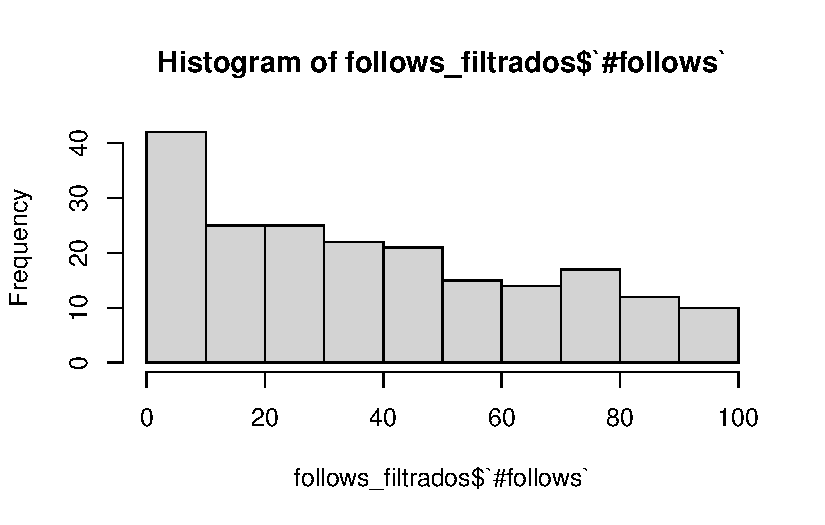
\includegraphics{analisisExploratorio_files/figure-pdf/unnamed-chunk-39-1.pdf}

Vemos que en este intervalo, si esta mas repartidas las frecuencias.

Viendo que hay algunos usuarios con un gran numero de cuentas seguidas,
no tiene sentido tomar el valor de la mediana como referencia ya que
esta no es significativa en este caso, por lo que vamos a analizar los
cuartiles y la mediana en su lugar.

\begin{Shaded}
\begin{Highlighting}[]
\FunctionTok{summary}\NormalTok{(datos}\SpecialCharTok{$}\StringTok{\textasciigrave{}}\AttributeTok{\#follows}\StringTok{\textasciigrave{}}\NormalTok{)}
\end{Highlighting}
\end{Shaded}

\begin{verbatim}
   Min. 1st Qu.  Median    Mean 3rd Qu.    Max. 
    0.0    57.5   229.5   508.4   589.5  7500.0 
\end{verbatim}

Ahora ya con estos valores ya podemos analizarlo un poco mejor y darnos
cuenta que el 50\% de los usuarios no sigue a mas de 229 cuentas.

\subsection{fake}\label{fake}

Por ultimo, este atributo es un atributo binario que representa si el
perfil es verdadero o es un spammer.

\begin{Shaded}
\begin{Highlighting}[]
\FunctionTok{hist}\NormalTok{(datos}\SpecialCharTok{$}\NormalTok{fake, }\AttributeTok{breaks =} \DecValTok{2}\NormalTok{, }\AttributeTok{main=}\StringTok{"Fake o no"}\NormalTok{ )}
\end{Highlighting}
\end{Shaded}

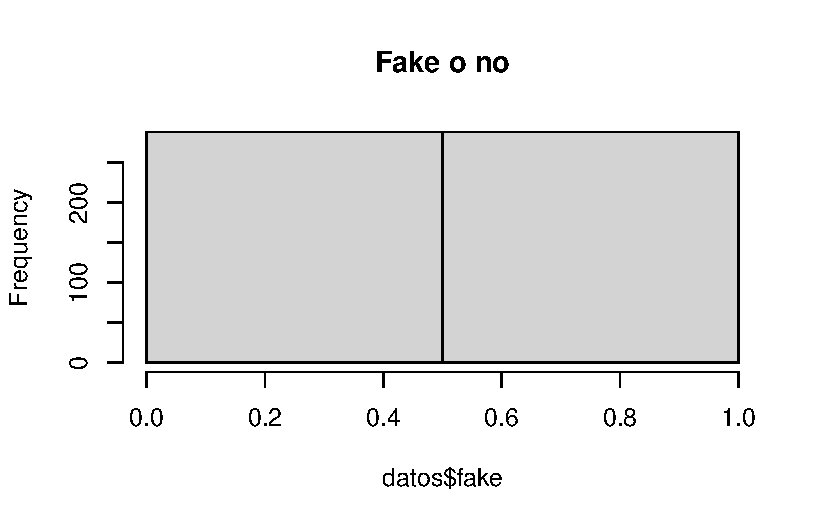
\includegraphics{analisisExploratorio_files/figure-pdf/unnamed-chunk-41-1.pdf}

Observamos que nuestro DataSet tiene un 50\% de cuentas falsas y otro
50\% de cuentas verdaderas.

\section{Herramienta de DataExplorer}\label{herramienta-de-dataexplorer}

\begin{Shaded}
\begin{Highlighting}[]
\FunctionTok{library}\NormalTok{(DataExplorer)}
\end{Highlighting}
\end{Shaded}

\begin{verbatim}
Warning: package 'DataExplorer' was built under R version 4.3.3
\end{verbatim}

\begin{Shaded}
\begin{Highlighting}[]
\CommentTok{\#create\_report(datos)}
\end{Highlighting}
\end{Shaded}

\begin{description}
\item[DataExplorer: Automate Data Exploration and Treatment]
Automated data exploration process for analytic tasks and predictive
modeling, so that users could focus on understanding data and extracting
insights. The package scans and analyzes each variable, and visualizes
them with typical graphical techniques. Common data processing methods
are also available to treat and format data.
\end{description}

La librería DataExplorer es una herramienta diseñada para simplificar y
acelerar el proceso de exploración y análisis de datos. Proporciona
funciones que permiten generar rápidamente resúmenes estadísticos,
visualizaciones y diagnósticos de los datos.

Algunas de las características clave incluyen la capacidad de generar
perfiles de datos detallados, identificar valores atípicos, analizar la
distribución de variables y explorar relaciones entre variables.

Podemos simplificar el proceso realizado anteriormente utilizando este
paquete.

\subsection{Funciones interesantes}\label{funciones-interesantes}

\subsubsection{introduce}\label{introduce}

Genera un pequeño reporte con los datos mas relevantes como el numero de
columnas, el tamano del datset, \ldots{}

\begin{Shaded}
\begin{Highlighting}[]
\FunctionTok{introduce}\NormalTok{(datos)}
\end{Highlighting}
\end{Shaded}

\begin{verbatim}
# A tibble: 1 x 9
   rows columns discrete_columns continuous_columns all_missing_columns
  <int>   <int>            <int>              <int>               <int>
1   576      12                0                 12                   0
# i 4 more variables: total_missing_values <int>, complete_rows <int>,
#   total_observations <int>, memory_usage <dbl>
\end{verbatim}

\begin{Shaded}
\begin{Highlighting}[]
\FunctionTok{plot\_intro}\NormalTok{(datos)}
\end{Highlighting}
\end{Shaded}

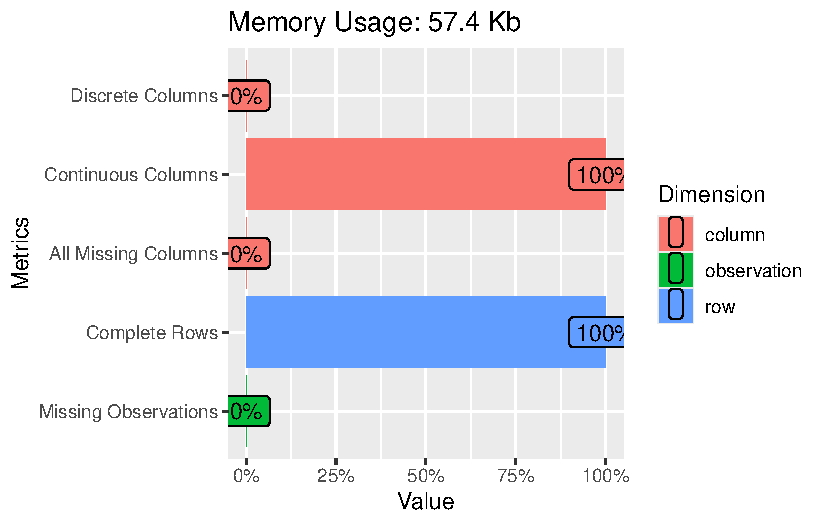
\includegraphics{analisisExploratorio_files/figure-pdf/unnamed-chunk-43-1.pdf}

\subsubsection{plot\_histogram}\label{plot_histogram}

Esta funcion nos muestra todos los histogramas de las
variables/columnas.

\begin{Shaded}
\begin{Highlighting}[]
\FunctionTok{plot\_histogram}\NormalTok{(datos)}
\end{Highlighting}
\end{Shaded}

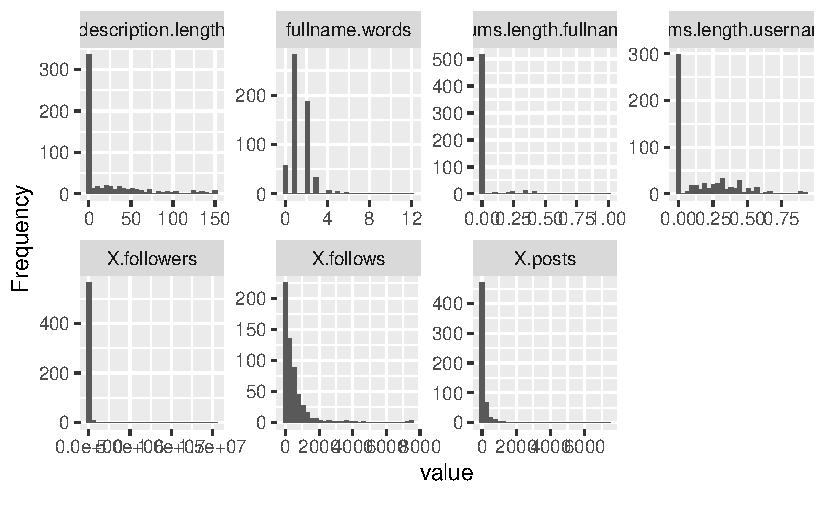
\includegraphics{analisisExploratorio_files/figure-pdf/unnamed-chunk-44-1.pdf}

\subsubsection{plot\_qq}\label{plot_qq}

Este comando genera un gráfico de cuantiles-cuantiles, el cual es una
forma de visualizar la desviación de una distribución de probabilidad
específica.

\begin{Shaded}
\begin{Highlighting}[]
\FunctionTok{plot\_qq}\NormalTok{(datos)}
\end{Highlighting}
\end{Shaded}

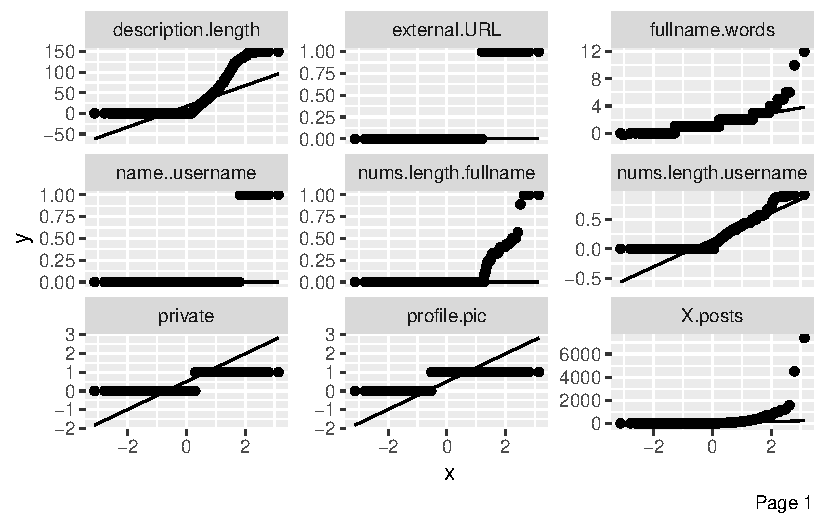
\includegraphics{analisisExploratorio_files/figure-pdf/unnamed-chunk-45-1.pdf}

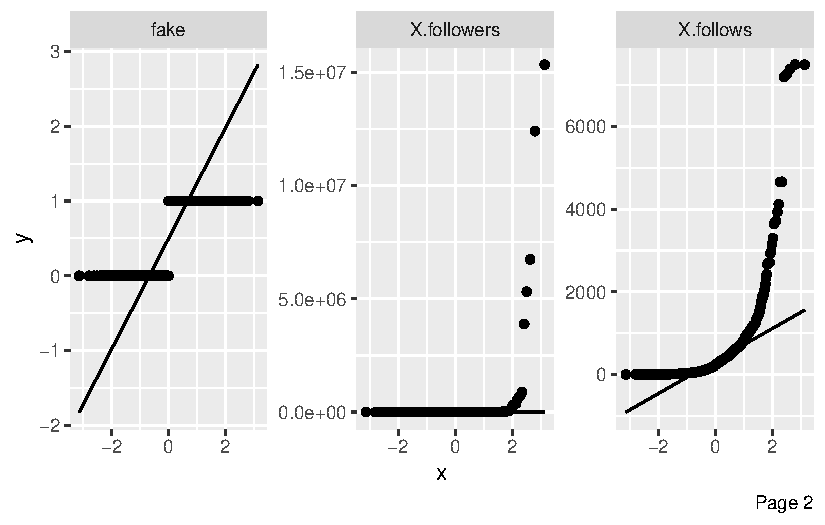
\includegraphics{analisisExploratorio_files/figure-pdf/unnamed-chunk-45-2.pdf}

\subsubsection{create\_report}\label{create_report}

Este comando realiza las medidas mencionadas anteriormente y muchas
otras que son útiles (como el análisis de componentes principales) para
el análisis exploratorio y genera como salida un reporte completo de
nuestros datos.

\begin{Shaded}
\begin{Highlighting}[]
\CommentTok{\#create\_report(datos)}
\end{Highlighting}
\end{Shaded}

\bookmarksetup{startatroot}

\chapter{Visualización de los
Datos}\label{visualizaciuxf3n-de-los-datos}

Ahora que ya hemos analizado en profundidad cada atributo de nuestro
DataSet, vamos a necesitar algunos gráficos que nos den ideas sobre como
continuar nuestro análisis.

Para ello vamos a utilizar al herramienta de \texttt{ggplot2} , la cual
nos va a permitir realizar los gráficos complejos de los que estamos
hablando.

\begin{description}
\item[ggplot2: Create Elegant Data Visualisations Using the Grammar of
Graphics]
A system for `declaratively' creating graphics, based on ``The Grammar
of Graphics''. You provide the data, tell `ggplot2' how to map variables
to aesthetics, what graphical primitives to use, and it takes care of
the details.
\end{description}

\href{https://ggplot2.tidyverse.org/}{Enlace a la librería}

Vamos a comenzar importando la librería y cargando nuestros datos.

\begin{Shaded}
\begin{Highlighting}[]
\FunctionTok{library}\NormalTok{(ggplot2)}
\FunctionTok{library}\NormalTok{(readr) }
\FunctionTok{library}\NormalTok{(magrittr)}
\FunctionTok{library}\NormalTok{(dplyr)}
\end{Highlighting}
\end{Shaded}

\begin{verbatim}

Attaching package: 'dplyr'
\end{verbatim}

\begin{verbatim}
The following objects are masked from 'package:stats':

    filter, lag
\end{verbatim}

\begin{verbatim}
The following objects are masked from 'package:base':

    intersect, setdiff, setequal, union
\end{verbatim}

\begin{Shaded}
\begin{Highlighting}[]
\NormalTok{datos }\OtherTok{\textless{}{-}} \FunctionTok{read\_csv}\NormalTok{(}\StringTok{"Data/train.csv"}\NormalTok{) }
\end{Highlighting}
\end{Shaded}

\begin{verbatim}
Rows: 576 Columns: 12
\end{verbatim}

\begin{verbatim}
-- Column specification --------------------------------------------------------
Delimiter: ","
dbl (12): profile pic, nums/length username, fullname words, nums/length ful...

i Use `spec()` to retrieve the full column specification for this data.
i Specify the column types or set `show_col_types = FALSE` to quiet this message.
\end{verbatim}

\section{Pre-procesado}\label{pre-procesado}

Para poder hacer este trabajo mas fácil, vamos a realizar un
pre-procesado de los datos primero. Vamos a convertir todos los
atributos que son discretos a factores:

\begin{Shaded}
\begin{Highlighting}[]
\NormalTok{datos\_refinados }\OtherTok{\textless{}{-}}\NormalTok{ datos}
\NormalTok{columnas\_binarias }\OtherTok{=} \FunctionTok{c}\NormalTok{(}\StringTok{"profile pic"}\NormalTok{,}\StringTok{"name==username"}\NormalTok{,}\StringTok{"external URL"}\NormalTok{,}\StringTok{"fake"}\NormalTok{,}\StringTok{"private"}\NormalTok{)}
\ControlFlowTok{for}\NormalTok{ (columna }\ControlFlowTok{in}\NormalTok{ columnas\_binarias) \{}
\NormalTok{  datos\_refinados[[columna]] }\OtherTok{\textless{}{-}}  \FunctionTok{factor}\NormalTok{(datos\_refinados[[columna]], }\AttributeTok{labels =} \FunctionTok{c}\NormalTok{(}\StringTok{"No"}\NormalTok{, }\StringTok{"Si"}\NormalTok{))}
\NormalTok{\}}
\end{Highlighting}
\end{Shaded}

Nuestro atributos discretos, son binarios, solo tienen o bien \emph{Si}
o \emph{No.} Vamos a emplear ahora los gráficos para poder encontrar
alguna relación entre las variables y sobre todo, lo que mas no
interesa, si alguna tiene relación con las cuentas de spam.

\section{Comparación de la cantidad de publicaciones entre cuentas
privadas y
públicas}\label{comparaciuxf3n-de-la-cantidad-de-publicaciones-entre-cuentas-privadas-y-puxfablicas}

Para ver como se comportan ambos tipos de usuarios, vamos a empezar
analizando el numero de publicaciones entre los usuarios con cuentas
publicas y con cuentas privadas, para ello vamos ver las densidades
utilizando \texttt{geom\_density} :

\begin{Shaded}
\begin{Highlighting}[]
\NormalTok{posts\_filtrados }\OtherTok{\textless{}{-}}\NormalTok{ datos\_refinados }\SpecialCharTok{\%\textgreater{}\%}  \FunctionTok{filter}\NormalTok{(}\StringTok{\textasciigrave{}}\AttributeTok{\#posts}\StringTok{\textasciigrave{}} \SpecialCharTok{\textless{}}\DecValTok{100}\NormalTok{)}

\FunctionTok{ggplot}\NormalTok{(}\AttributeTok{data =}\NormalTok{ posts\_filtrados, }\FunctionTok{aes}\NormalTok{( }\AttributeTok{x =} \StringTok{\textasciigrave{}}\AttributeTok{\#posts}\StringTok{\textasciigrave{}}\NormalTok{,}\AttributeTok{fill =}\NormalTok{ private)) }\SpecialCharTok{+}
  \FunctionTok{geom\_density}\NormalTok{(}\AttributeTok{alpha =} \FloatTok{0.5}\NormalTok{) }\SpecialCharTok{+}
  \FunctionTok{labs}\NormalTok{(}\AttributeTok{title =} \StringTok{"Comparación de publicaciones entre cuentas privadas y públicas"}\NormalTok{,}
       \AttributeTok{x =} \StringTok{"Numero de publicacion"}\NormalTok{,}
       \AttributeTok{y =} \StringTok{"Densidad"}\NormalTok{) }\SpecialCharTok{+}
  \FunctionTok{scale\_fill\_manual}\NormalTok{(}\AttributeTok{values =} \FunctionTok{c}\NormalTok{(}\StringTok{"lightgreen"}\NormalTok{, }\StringTok{"lightcoral"}\NormalTok{))}
\end{Highlighting}
\end{Shaded}

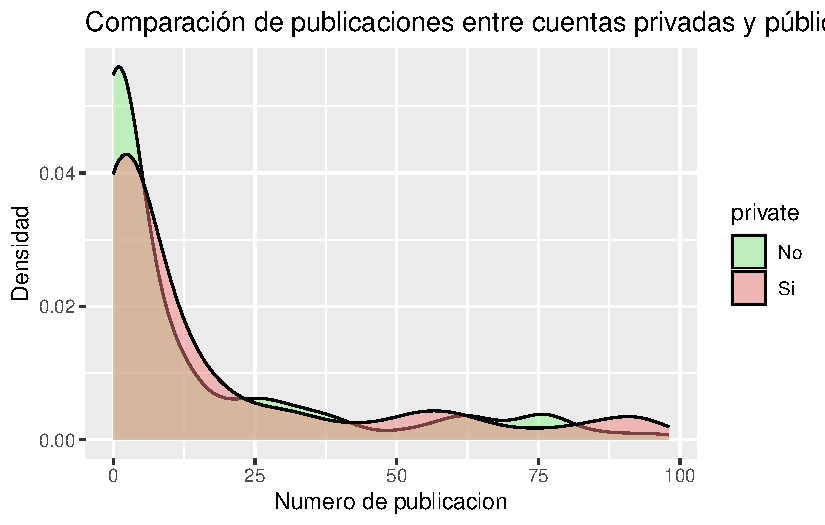
\includegraphics{visualizacionDatos_files/figure-pdf/unnamed-chunk-3-1.pdf}

Vemos que ambos casos, nuestra gráfica se asemeja, por lo que el numero
de publicaciones no depende de si es privada o publica.

Sin embargo, realmente a nosotros nos interese encontrar relaciones para
intentar determinar si una cuenta es spammer o de un persona real. Por
lo tanto vamos a centrarnos en comparar los atributos con el atributos
spam.

\section{Relación entre visibilidad del perfil y cuentas
fake}\label{relaciuxf3n-entre-visibilidad-del-perfil-y-cuentas-fake}

Como nos interesa buscar las cuentas de spam, vamos a ver si la
visibilidad del perfil (cuenta privada o publica), tiene algo que ver:

\begin{Shaded}
\begin{Highlighting}[]
\FunctionTok{ggplot}\NormalTok{(datos\_refinados, }\FunctionTok{aes}\NormalTok{(}\AttributeTok{x =} \StringTok{\textasciigrave{}}\AttributeTok{fake}\StringTok{\textasciigrave{}}\NormalTok{, }\AttributeTok{y =} \StringTok{\textasciigrave{}}\AttributeTok{private}\StringTok{\textasciigrave{}}\NormalTok{)) }\SpecialCharTok{+}   
  \FunctionTok{geom\_count}\NormalTok{(}\AttributeTok{color =} \StringTok{"blue"}\NormalTok{, }\AttributeTok{alpha =} \FloatTok{0.6}\NormalTok{) }\SpecialCharTok{+}   
  \FunctionTok{scale\_size\_area}\NormalTok{()}\SpecialCharTok{+}   
  \FunctionTok{labs}\NormalTok{(}\AttributeTok{title =} \StringTok{"Relación entre visibilidad del perfil y si es spam"}\NormalTok{,        }
       \AttributeTok{x =} \StringTok{"Cuenta fake"}\NormalTok{,        }
       \AttributeTok{y =} \StringTok{"Cuenta privada"}\NormalTok{)}\SpecialCharTok{+}   
  \FunctionTok{theme\_minimal}\NormalTok{() }
\end{Highlighting}
\end{Shaded}

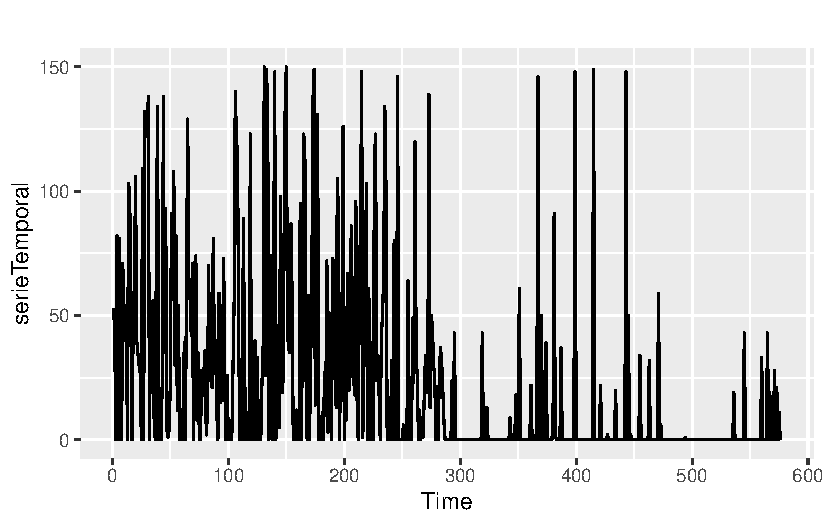
\includegraphics{visualizacionDatos_files/figure-pdf/unnamed-chunk-4-1.pdf}

Utilizando \texttt{geom\_count} con dos variables discretas, en este
caso si un perfil es privado o no y si un perfil es fake o no, no
podemos extraer mucha información relevante ya que vemos que hay
aproximadamente un numero similar de cada combinación.

\section{Relación entre tener foto de perfil y ser cuenta
fake}\label{relaciuxf3n-entre-tener-foto-de-perfil-y-ser-cuenta-fake}

Al igual que antes vamos a comprobar dos variables discretas, por lo que
el aspecto del gráfico sera diferente. Vamos a comprobar si tener o no
foto de perfil tiene algo de relación con ser un spammer.

\begin{Shaded}
\begin{Highlighting}[]
\FunctionTok{ggplot}\NormalTok{(datos\_refinados, }\FunctionTok{aes}\NormalTok{(}\AttributeTok{x =} \StringTok{\textasciigrave{}}\AttributeTok{fake}\StringTok{\textasciigrave{}}\NormalTok{, }\AttributeTok{y =} \StringTok{\textasciigrave{}}\AttributeTok{profile pic}\StringTok{\textasciigrave{}}\NormalTok{)) }\SpecialCharTok{+}   
  \FunctionTok{geom\_jitter}\NormalTok{(}\AttributeTok{color =} \StringTok{"blue"}\NormalTok{, }\AttributeTok{alpha =} \FloatTok{0.6}\NormalTok{) }\SpecialCharTok{+}   
  \FunctionTok{scale\_size\_area}\NormalTok{()}\SpecialCharTok{+}   
  \FunctionTok{labs}\NormalTok{(}\AttributeTok{title =} \StringTok{"Relación entre tener foto de perfil y si es spam"}\NormalTok{,        }
       \AttributeTok{x =} \StringTok{"Cuenta fake"}\NormalTok{,        }
       \AttributeTok{y =} \StringTok{"Foto de perfil"}\NormalTok{)}\SpecialCharTok{+}   
  \FunctionTok{theme\_minimal}\NormalTok{() }
\end{Highlighting}
\end{Shaded}

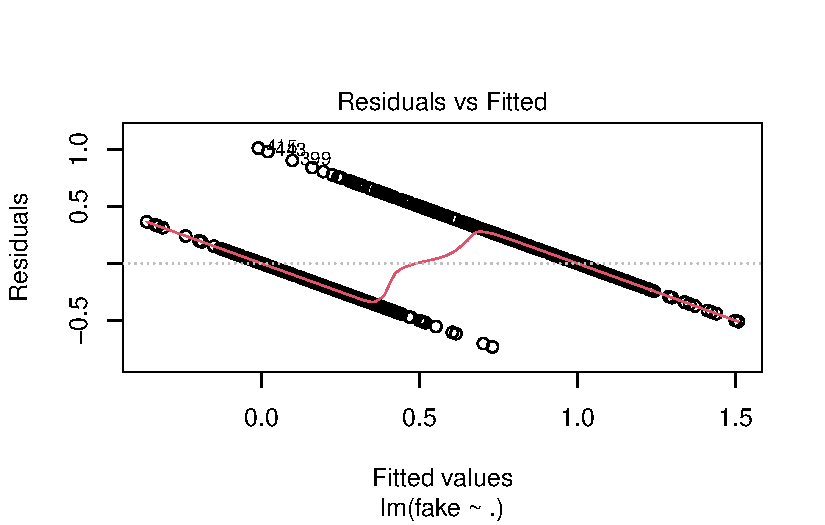
\includegraphics{visualizacionDatos_files/figure-pdf/unnamed-chunk-5-1.pdf}

Hemos obtenido un resultado interesante, donde vemos que las cuentas
reales, todas menos 2 tienen foto de perfil puesta, mientras que las
cuentas fake hay mas o menos un mismo numero con foto de perfil y sin
foto de perfil. Estos datos, combinados con otros que vamos a obtener
mas adelante, nos pueden ayudar a diferenciar cuentas reales de falsas.

\section{Relación entre numero de publicaciones y cuentas
fake}\label{relaciuxf3n-entre-numero-de-publicaciones-y-cuentas-fake}

Podemos suponer una posible hipótesis en la que los usuarios spammers,
cuya tarea puede ser solo generar comentarios o likes, van a tener
cuentas con menos numero de publicaciones que una cuenta de una persona
verdadera. Vamos a visualizar esta idea:

\begin{Shaded}
\begin{Highlighting}[]
\NormalTok{posts\_filtrados }\OtherTok{\textless{}{-}}\NormalTok{ datos\_refinados }\SpecialCharTok{\%\textgreater{}\%}  \FunctionTok{filter}\NormalTok{(}\StringTok{\textasciigrave{}}\AttributeTok{\#posts}\StringTok{\textasciigrave{}} \SpecialCharTok{\textless{}}\DecValTok{100}\NormalTok{)}
\FunctionTok{ggplot}\NormalTok{(posts\_filtrados, }\FunctionTok{aes}\NormalTok{(}\AttributeTok{x =}\NormalTok{ fake, }\AttributeTok{y =} \StringTok{\textasciigrave{}}\AttributeTok{\#posts}\StringTok{\textasciigrave{}}\NormalTok{)) }\SpecialCharTok{+}
  \FunctionTok{geom\_violin}\NormalTok{(}\AttributeTok{fill =} \StringTok{"skyblue"}\NormalTok{, }\AttributeTok{color =} \StringTok{"black"}\NormalTok{) }
\end{Highlighting}
\end{Shaded}

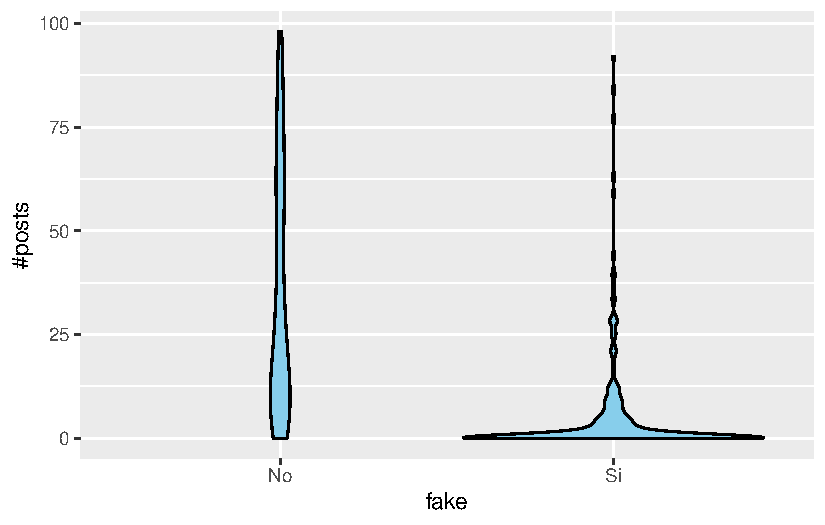
\includegraphics{visualizacionDatos_files/figure-pdf/unnamed-chunk-6-1.pdf}

Observamos que teníamos razón, despues de eliminar aquellas cuentas con
muchos post, vemos que las cuentas falsas suelen tener un numero
reducido de publicaciones, mientras que las cuentas normales suelen
tener una distribución mas uniforme.

\section{Análisis de numero de
seguidores}\label{anuxe1lisis-de-numero-de-seguidores}

Unos de los atributos mas relevantes pueden ser el numero de seguidores
el numero de seguidos, por lo quenecesitamos analizarlos en profundidad.
Vamos a comenzar con el numero de seguidores.

Primero, como en el análisis exploratorio observamos que había algunas
cuentas con muchos seguidores pero que no representaban un numero
importante, vamos a eliminar esas escasas cuentas con un numero alto de
seguidores con el fin de que los gráficos sean mas entendibles.

\begin{Shaded}
\begin{Highlighting}[]
\NormalTok{followers\_filtrados }\OtherTok{\textless{}{-}}\NormalTok{ datos\_refinados }\SpecialCharTok{\%\textgreater{}\%} \FunctionTok{filter}\NormalTok{(}\StringTok{\textasciigrave{}}\AttributeTok{\#followers}\StringTok{\textasciigrave{}} \SpecialCharTok{\textless{}}\DecValTok{1500}\NormalTok{)}

\FunctionTok{ggplot}\NormalTok{(followers\_filtrados, }\FunctionTok{aes}\NormalTok{(}\AttributeTok{x =} \StringTok{\textasciigrave{}}\AttributeTok{\#followers}\StringTok{\textasciigrave{}}\NormalTok{)) }\SpecialCharTok{+}
  \FunctionTok{geom\_histogram}\NormalTok{(}\AttributeTok{binwidth =} \DecValTok{10}\NormalTok{, }\AttributeTok{color =} \StringTok{\textquotesingle{}black\textquotesingle{}}\NormalTok{) }\SpecialCharTok{+}
    \FunctionTok{labs}\NormalTok{(}\AttributeTok{title =} \StringTok{"Histograma de seguidores"}\NormalTok{,}
       \AttributeTok{x =} \StringTok{"Cantidad de Seguidores"}\NormalTok{,}
       \AttributeTok{y =} \StringTok{"Frecuencias"}\NormalTok{)}
\end{Highlighting}
\end{Shaded}

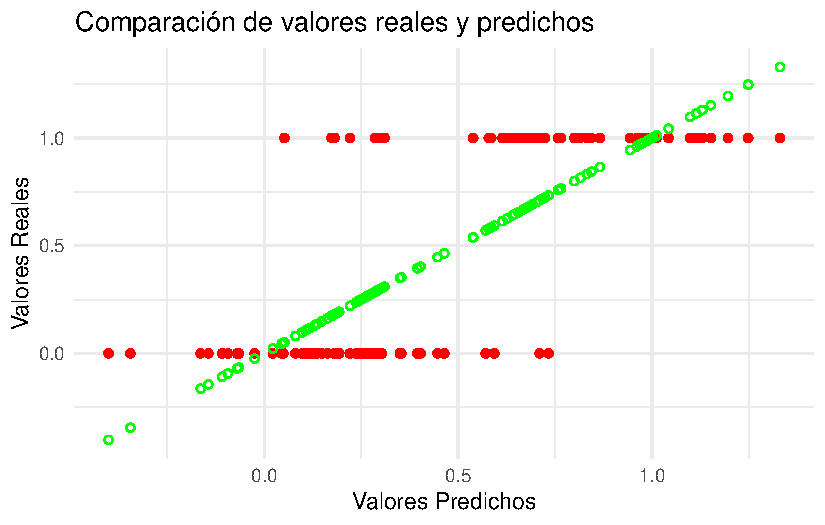
\includegraphics{visualizacionDatos_files/figure-pdf/unnamed-chunk-7-1.pdf}

Vemos que se concentra la mayoría en menos de 250 seguidores.

Vamos a utilizar una gráfica de frecuencia para ver como son nuestros
datos con menos de 250 seguidores.

\begin{Shaded}
\begin{Highlighting}[]
\NormalTok{followers\_filtrados }\OtherTok{\textless{}{-}}\NormalTok{ datos\_refinados }\SpecialCharTok{\%\textgreater{}\%}  \FunctionTok{filter}\NormalTok{(}\StringTok{\textasciigrave{}}\AttributeTok{\#followers}\StringTok{\textasciigrave{}} \SpecialCharTok{\textless{}}\DecValTok{250}\NormalTok{)}

\FunctionTok{ggplot}\NormalTok{(followers\_filtrados, }\FunctionTok{aes}\NormalTok{(}\AttributeTok{x =} \StringTok{\textasciigrave{}}\AttributeTok{\#followers}\StringTok{\textasciigrave{}}\NormalTok{)) }\SpecialCharTok{+}
  \FunctionTok{geom\_freqpoly}\NormalTok{(}\AttributeTok{color =} \StringTok{"blue"}\NormalTok{, }\AttributeTok{binwidth =} \DecValTok{5}\NormalTok{) }\SpecialCharTok{+}
  \FunctionTok{labs}\NormalTok{(}\AttributeTok{title =} \StringTok{"Distribución de la Cantidad de Seguidores"}\NormalTok{,}
       \AttributeTok{x =} \StringTok{"Cantidad de Seguidores"}\NormalTok{,}
       \AttributeTok{y =} \StringTok{"Frecuencia"}\NormalTok{) }
\end{Highlighting}
\end{Shaded}

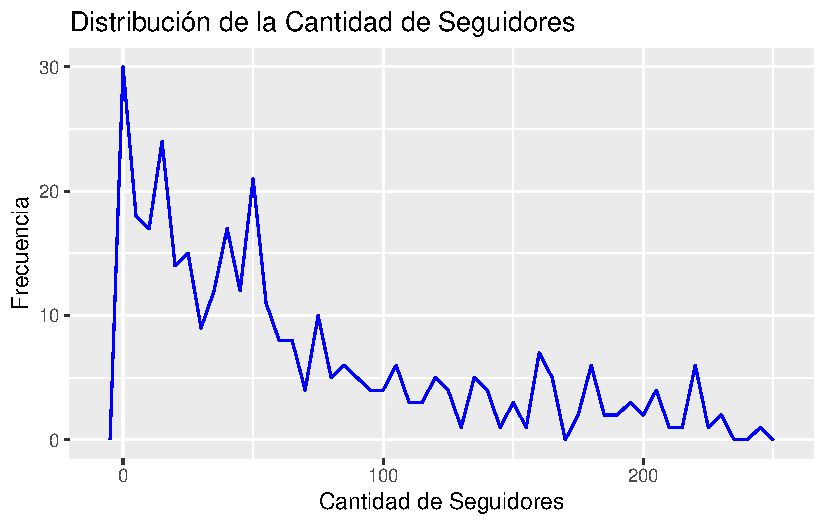
\includegraphics{visualizacionDatos_files/figure-pdf/unnamed-chunk-8-1.pdf}

La mayor concentración se encuentra en menos de 100 seguidores y que es
decreciente la frecuencia a medida que aumenta el numero de seguidores.

\subsection{Comparación del numero de seguidores entre cuentas reales y
falsas}\label{comparaciuxf3n-del-numero-de-seguidores-entre-cuentas-reales-y-falsas}

Como nuestro principal objetivo es poder encontrar características
similares que tengan las cuentas falsas para poder encontrarlas
fácilmente, vamos a visualizar este atributo en relación con el numero
de seguidores. Ademas añadimos las medias para obtener mas información.

\begin{Shaded}
\begin{Highlighting}[]
\NormalTok{mean\_values }\OtherTok{\textless{}{-}}\NormalTok{ followers\_filtrados }\SpecialCharTok{\%\textgreater{}\%} 
  \FunctionTok{group\_by}\NormalTok{(fake) }\SpecialCharTok{\%\textgreater{}\%} 
  \FunctionTok{summarize}\NormalTok{(}\AttributeTok{mean\_followerss =} \FunctionTok{mean}\NormalTok{(}\StringTok{\textasciigrave{}}\AttributeTok{\#followers}\StringTok{\textasciigrave{}}\NormalTok{))}

\FunctionTok{ggplot}\NormalTok{(}\AttributeTok{data =}\NormalTok{ followers\_filtrados, }\FunctionTok{aes}\NormalTok{( }\AttributeTok{x =} \StringTok{\textasciigrave{}}\AttributeTok{\#followers}\StringTok{\textasciigrave{}}\NormalTok{,}\AttributeTok{fill =} \StringTok{\textasciigrave{}}\AttributeTok{fake}\StringTok{\textasciigrave{}}\NormalTok{)) }\SpecialCharTok{+}   \FunctionTok{geom\_density}\NormalTok{(}\AttributeTok{alpha =} \FloatTok{0.5}\NormalTok{) }\SpecialCharTok{+}   
  \FunctionTok{labs}\NormalTok{(}\AttributeTok{title =} \StringTok{"Comparación de seguidores entre cuentas reales y falsas"}\NormalTok{,        }
       \AttributeTok{x =} \StringTok{"Numero de seguidores"}\NormalTok{,        }
       \AttributeTok{y =} \StringTok{"Densidad"}\NormalTok{) }\SpecialCharTok{+}   
  \FunctionTok{scale\_fill\_manual}\NormalTok{(}\AttributeTok{values =} \FunctionTok{c}\NormalTok{(}\StringTok{"lightgreen"}\NormalTok{, }\StringTok{"lightcoral"}\NormalTok{))}\SpecialCharTok{+}
  \FunctionTok{geom\_vline}\NormalTok{(}\AttributeTok{data =}\NormalTok{ mean\_values, }\FunctionTok{aes}\NormalTok{(}\AttributeTok{xintercept =}\NormalTok{ mean\_followerss, }\AttributeTok{color =}\NormalTok{ fake), }\AttributeTok{linetype =} \StringTok{"dashed"}\NormalTok{, }\AttributeTok{size =} \DecValTok{1}\NormalTok{) }\SpecialCharTok{+}
   \FunctionTok{geom\_text}\NormalTok{(}\AttributeTok{data =}\NormalTok{ mean\_values, }\FunctionTok{aes}\NormalTok{(}\AttributeTok{x =}\NormalTok{ mean\_followerss, }\AttributeTok{y =} \DecValTok{0}\NormalTok{, }\AttributeTok{label =} \FunctionTok{round}\NormalTok{(mean\_followerss, }\DecValTok{1}\NormalTok{), }\AttributeTok{color =}\NormalTok{ fake),}
            \AttributeTok{vjust =} \SpecialCharTok{{-}}\FloatTok{0.5}\NormalTok{, }\AttributeTok{hjust =} \SpecialCharTok{{-}}\FloatTok{0.1}\NormalTok{, }\AttributeTok{size =} \DecValTok{4}\NormalTok{, }\AttributeTok{fontface =} \StringTok{"bold"}\NormalTok{) }\SpecialCharTok{+}
  \FunctionTok{scale\_color\_manual}\NormalTok{(}\AttributeTok{values =} \FunctionTok{c}\NormalTok{(}\StringTok{"lightgreen"}\NormalTok{, }\StringTok{"lightcoral"}\NormalTok{), }\AttributeTok{name =} \StringTok{"Media"}\NormalTok{)}
\end{Highlighting}
\end{Shaded}

\begin{verbatim}
Warning: Using `size` aesthetic for lines was deprecated in ggplot2 3.4.0.
i Please use `linewidth` instead.
\end{verbatim}

\includegraphics{visualizacionDatos_files/figure-pdf/unnamed-chunk-9-1.pdf}

Aquí y obtenemos información mas interesante. Podemos observar que las
cuentas falsas tienen a tener un menor numero de seguidores, mientras
que las cuentas reales, aunque no tienen muchos seguidores, se suelen
mantener en un intervalo entre 50 y 250. Esta información nos puede ser
de importancia para los cálculos futuros.

\section{Análisis de numero de
seguidos}\label{anuxe1lisis-de-numero-de-seguidos}

Ahora que hemos ya explorados gracias a varios gráficos como se comporta
el numero de seguidores segun el tipo de cuentas, vamos a continuar
ahora con el numero de seguidos.

Primero, como en el análisis exploratorio observamos que había algunas
cuentas con muchos seguidos, pero que no representaban un numero
importante, vamos a eliminar esas escasas cuentas con un numero alto de
seguidos con el fin de que los gráficos sean mas entendibles.

\begin{Shaded}
\begin{Highlighting}[]
\NormalTok{follows\_filtrados }\OtherTok{\textless{}{-}}\NormalTok{ datos\_refinados }\SpecialCharTok{\%\textgreater{}\%}  \FunctionTok{filter}\NormalTok{(}\StringTok{\textasciigrave{}}\AttributeTok{\#follows}\StringTok{\textasciigrave{}} \SpecialCharTok{\textless{}}\DecValTok{1000}\NormalTok{)  }
\FunctionTok{ggplot}\NormalTok{(follows\_filtrados, }\FunctionTok{aes}\NormalTok{(}\AttributeTok{x =} \StringTok{\textasciigrave{}}\AttributeTok{\#follows}\StringTok{\textasciigrave{}}\NormalTok{)) }\SpecialCharTok{+}   \FunctionTok{geom\_histogram}\NormalTok{(}\AttributeTok{binwidth =} \DecValTok{10}\NormalTok{, }\AttributeTok{color =} \StringTok{\textquotesingle{}black\textquotesingle{}}\NormalTok{) }\SpecialCharTok{+}     
  \FunctionTok{labs}\NormalTok{(}\AttributeTok{title =} \StringTok{"Histograma de seguidos"}\NormalTok{,        }
       \AttributeTok{x =} \StringTok{"Cantidad de Seguidos"}\NormalTok{,        }
       \AttributeTok{y =} \StringTok{"Frecuencias"}\NormalTok{)}
\end{Highlighting}
\end{Shaded}

\includegraphics{visualizacionDatos_files/figure-pdf/unnamed-chunk-10-1.pdf}

Vemos que se concentra la mayoría en menos de 250 seguidos.

Vamos a utilizar una gráfica de frecuencia para ver como son nuestros
datos con menos de 250 seguidos.

\begin{Shaded}
\begin{Highlighting}[]
\NormalTok{follows\_filtrados }\OtherTok{\textless{}{-}}\NormalTok{ datos\_refinados }\SpecialCharTok{\%\textgreater{}\%}  \FunctionTok{filter}\NormalTok{(}\StringTok{\textasciigrave{}}\AttributeTok{\#follows}\StringTok{\textasciigrave{}} \SpecialCharTok{\textless{}}\DecValTok{250}\NormalTok{)   }
\FunctionTok{ggplot}\NormalTok{(follows\_filtrados, }\FunctionTok{aes}\NormalTok{(}\AttributeTok{x =} \StringTok{\textasciigrave{}}\AttributeTok{\#follows}\StringTok{\textasciigrave{}}\NormalTok{)) }\SpecialCharTok{+}   
  \FunctionTok{geom\_freqpoly}\NormalTok{(}\AttributeTok{color =} \StringTok{"blue"}\NormalTok{, }\AttributeTok{binwidth =} \DecValTok{5}\NormalTok{) }\SpecialCharTok{+}   
  \FunctionTok{labs}\NormalTok{(}\AttributeTok{title =} \StringTok{"Distribución de la Cantidad de Seguidos"}\NormalTok{,        }
       \AttributeTok{x =} \StringTok{"Cantidad de Seguidos"}\NormalTok{,        }
       \AttributeTok{y =} \StringTok{"Frecuencia"}\NormalTok{)  }
\end{Highlighting}
\end{Shaded}

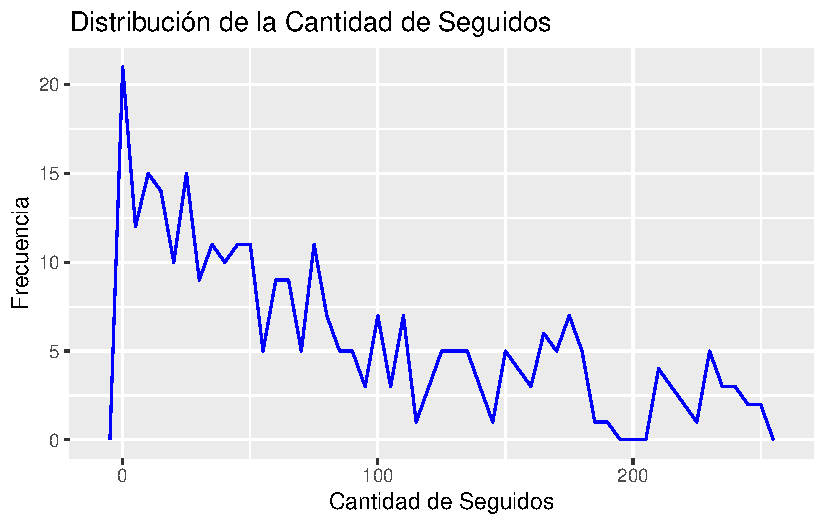
\includegraphics{visualizacionDatos_files/figure-pdf/unnamed-chunk-11-1.pdf}

La mayor concentración se encuentra en menos de 100 seguidos y que es
decreciente la frecuencia a medida que aumenta el numero de seguidores.

\subsection{Comparación del numero de seguidos entre cuentas reales y
falsas}\label{comparaciuxf3n-del-numero-de-seguidos-entre-cuentas-reales-y-falsas}

Como nuestro principal objetivo es poder encontrar características
similares que tengan las cuentas falsas para poder encontrarlas
fácilmente, vamos a visualizar este atributo. Ademas añadimos las medias
para obtener mas información.

\begin{Shaded}
\begin{Highlighting}[]
\NormalTok{follows\_filtrados }\OtherTok{\textless{}{-}}\NormalTok{ datos\_refinados }\SpecialCharTok{\%\textgreater{}\%}  \FunctionTok{filter}\NormalTok{(}\StringTok{\textasciigrave{}}\AttributeTok{\#follows}\StringTok{\textasciigrave{}} \SpecialCharTok{\textless{}}\DecValTok{550}\NormalTok{)  }

\NormalTok{mean\_values }\OtherTok{\textless{}{-}}\NormalTok{ follows\_filtrados }\SpecialCharTok{\%\textgreater{}\%} 
  \FunctionTok{group\_by}\NormalTok{(fake) }\SpecialCharTok{\%\textgreater{}\%} 
  \FunctionTok{summarize}\NormalTok{(}\AttributeTok{mean\_follows =} \FunctionTok{mean}\NormalTok{(}\StringTok{\textasciigrave{}}\AttributeTok{\#follows}\StringTok{\textasciigrave{}}\NormalTok{))}

\FunctionTok{ggplot}\NormalTok{(}\AttributeTok{data =}\NormalTok{ follows\_filtrados, }\FunctionTok{aes}\NormalTok{( }\AttributeTok{x =} \StringTok{\textasciigrave{}}\AttributeTok{\#follows}\StringTok{\textasciigrave{}}\NormalTok{,}\AttributeTok{fill =} \StringTok{\textasciigrave{}}\AttributeTok{fake}\StringTok{\textasciigrave{}}\NormalTok{)) }\SpecialCharTok{+}   \FunctionTok{geom\_density}\NormalTok{(}\AttributeTok{alpha =} \FloatTok{0.5}\NormalTok{) }\SpecialCharTok{+}   
  \FunctionTok{labs}\NormalTok{(}\AttributeTok{title =} \StringTok{"Comparación de seguidos entre cuentas reales y falsas"}\NormalTok{,        }
       \AttributeTok{x =} \StringTok{"Numero de seguidos"}\NormalTok{,        }
       \AttributeTok{y =} \StringTok{"Densidad"}\NormalTok{) }\SpecialCharTok{+}   
  \FunctionTok{scale\_fill\_manual}\NormalTok{(}\AttributeTok{values =} \FunctionTok{c}\NormalTok{(}\StringTok{"lightgreen"}\NormalTok{, }\StringTok{"lightcoral"}\NormalTok{))}\SpecialCharTok{+}
  \FunctionTok{geom\_vline}\NormalTok{(}\AttributeTok{data =}\NormalTok{ mean\_values, }\FunctionTok{aes}\NormalTok{(}\AttributeTok{xintercept =}\NormalTok{ mean\_follows, }\AttributeTok{color =}\NormalTok{ fake), }\AttributeTok{linetype =} \StringTok{"dashed"}\NormalTok{, }\AttributeTok{size =} \DecValTok{1}\NormalTok{) }\SpecialCharTok{+}
   \FunctionTok{geom\_text}\NormalTok{(}\AttributeTok{data =}\NormalTok{ mean\_values, }\FunctionTok{aes}\NormalTok{(}\AttributeTok{x =}\NormalTok{ mean\_follows, }\AttributeTok{y =} \DecValTok{0}\NormalTok{, }\AttributeTok{label =} \FunctionTok{round}\NormalTok{(mean\_follows, }\DecValTok{1}\NormalTok{), }\AttributeTok{color =}\NormalTok{ fake),}
            \AttributeTok{vjust =} \SpecialCharTok{{-}}\FloatTok{0.5}\NormalTok{, }\AttributeTok{hjust =} \SpecialCharTok{{-}}\FloatTok{0.1}\NormalTok{, }\AttributeTok{size =} \DecValTok{4}\NormalTok{, }\AttributeTok{fontface =} \StringTok{"bold"}\NormalTok{) }\SpecialCharTok{+}
  \FunctionTok{scale\_color\_manual}\NormalTok{(}\AttributeTok{values =} \FunctionTok{c}\NormalTok{(}\StringTok{"lightgreen"}\NormalTok{, }\StringTok{"lightcoral"}\NormalTok{), }\AttributeTok{name =} \StringTok{"Media"}\NormalTok{)}
\end{Highlighting}
\end{Shaded}

\includegraphics{visualizacionDatos_files/figure-pdf/unnamed-chunk-12-1.pdf}

Aquí, al igual que con lo seguidores, obtenemos información mas
interesante. Podemos observar que las cuentas falsas tienen a tener un
menor numero de seguidores, pero no tan cercano al 0, mientras que las
cuentas reales, suelen tener un numero mas repartido de seguidos. Esta
información nos puede ser de importancia para los cálculos futuros.

\section{Relación entre numero de seguidores y numero de
seguidos}\label{relaciuxf3n-entre-numero-de-seguidores-y-numero-de-seguidos}

Ahora que la hemos visto ambas variables por separado, vamos a utilizar
los gráficos de puntos o dispersión para ver varias variables juntas
para intentar ver alguna relación o característica en estas.

\begin{Shaded}
\begin{Highlighting}[]
\NormalTok{followers\_filtrados }\OtherTok{\textless{}{-}}\NormalTok{ datos\_refinados }\SpecialCharTok{\%\textgreater{}\%}  \FunctionTok{filter}\NormalTok{(}\StringTok{\textasciigrave{}}\AttributeTok{\#followers}\StringTok{\textasciigrave{}} \SpecialCharTok{\textless{}}\DecValTok{5000}\NormalTok{)}


\FunctionTok{ggplot}\NormalTok{(}\AttributeTok{data =}\NormalTok{ followers\_filtrados, }\FunctionTok{aes}\NormalTok{(}\AttributeTok{x =} \StringTok{\textasciigrave{}}\AttributeTok{\#follows}\StringTok{\textasciigrave{}}\NormalTok{, }\AttributeTok{y =} \StringTok{\textasciigrave{}}\AttributeTok{\#followers}\StringTok{\textasciigrave{}}\NormalTok{)) }\SpecialCharTok{+}
  \FunctionTok{geom\_point}\NormalTok{(}\AttributeTok{shape =} \DecValTok{4}\NormalTok{, }\AttributeTok{size =} \DecValTok{3}\NormalTok{) }\SpecialCharTok{+}
  \FunctionTok{labs}\NormalTok{(}\AttributeTok{title =} \StringTok{"Seguidores vs. Seguidos"}\NormalTok{,}
       \AttributeTok{x =} \StringTok{"Cantidad de Seguidos"}\NormalTok{,}
       \AttributeTok{y =} \StringTok{"Cantidad de Seguidores"}\NormalTok{)}\SpecialCharTok{+}
  \FunctionTok{scale\_fill\_manual}\NormalTok{(}\AttributeTok{values =} \FunctionTok{c}\NormalTok{(}\StringTok{"skyblue"}\NormalTok{, }\StringTok{"lightcoral"}\NormalTok{))}
\end{Highlighting}
\end{Shaded}

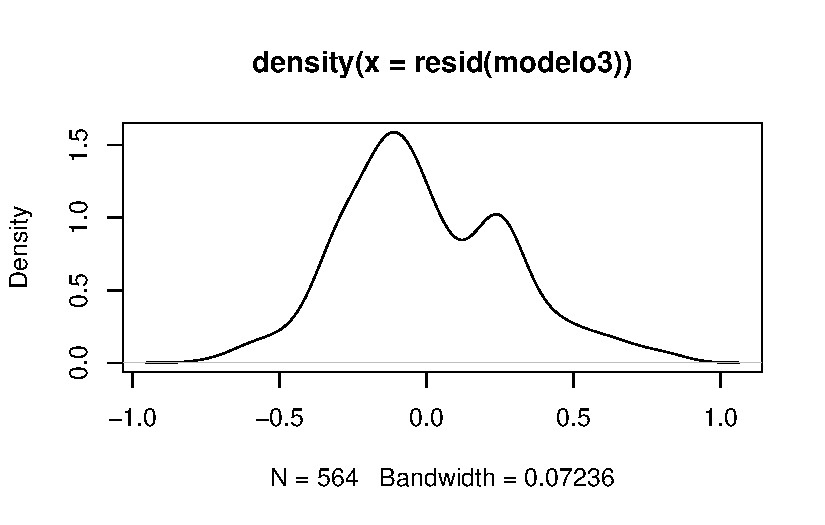
\includegraphics{visualizacionDatos_files/figure-pdf/unnamed-chunk-13-1.pdf}

Viendo este gráfico solo podemos obtener que casi todo se concentra a un
numero reducido tanto de seguidos y seguidores.

Aunque dicha información no nos sirve de mucho, vamos a añadir el
parametro para diferenciar cuentas fake y reales. Podemos pensar que los
seguidores y los seguidos tienen algo de relación con los usuarios que
son fake, vamos a refinar un poco el DataSet eliminando los usuarios que
tenian muchos seguidores, vamos a investigar:

\begin{Shaded}
\begin{Highlighting}[]
\NormalTok{followers\_filtrados }\OtherTok{\textless{}{-}}\NormalTok{ datos\_refinados }\SpecialCharTok{\%\textgreater{}\%}  \FunctionTok{filter}\NormalTok{(}\StringTok{\textasciigrave{}}\AttributeTok{\#followers}\StringTok{\textasciigrave{}} \SpecialCharTok{\textless{}}\DecValTok{5000}\NormalTok{)}


\FunctionTok{ggplot}\NormalTok{(}\AttributeTok{data =}\NormalTok{ followers\_filtrados, }\FunctionTok{aes}\NormalTok{(}\AttributeTok{x =} \StringTok{\textasciigrave{}}\AttributeTok{\#follows}\StringTok{\textasciigrave{}}\NormalTok{, }\AttributeTok{y =} \StringTok{\textasciigrave{}}\AttributeTok{\#followers}\StringTok{\textasciigrave{}}\NormalTok{, }\AttributeTok{fill =}\NormalTok{fake)) }\SpecialCharTok{+}
  \FunctionTok{geom\_point}\NormalTok{(}\AttributeTok{shape =} \DecValTok{21}\NormalTok{, }\AttributeTok{size =} \DecValTok{3}\NormalTok{) }\SpecialCharTok{+}
  \FunctionTok{labs}\NormalTok{(}\AttributeTok{title =} \StringTok{"Seguidores vs. Seguidos con Relleno según \textquotesingle{}Fake\textquotesingle{}"}\NormalTok{,}
       \AttributeTok{x =} \StringTok{"Cantidad de Seguidos"}\NormalTok{,}
       \AttributeTok{y =} \StringTok{"Cantidad de Seguidores"}\NormalTok{,}
       \AttributeTok{fill =} \StringTok{"Fake"}\NormalTok{) }\SpecialCharTok{+}
  \FunctionTok{scale\_fill\_manual}\NormalTok{(}\AttributeTok{values =} \FunctionTok{c}\NormalTok{(}\StringTok{"skyblue"}\NormalTok{, }\StringTok{"lightcoral"}\NormalTok{), }\AttributeTok{labels =} \FunctionTok{c}\NormalTok{(}\StringTok{"Real"}\NormalTok{, }\StringTok{"Falso"}\NormalTok{))}
\end{Highlighting}
\end{Shaded}

\includegraphics{visualizacionDatos_files/figure-pdf/unnamed-chunk-14-1.pdf}

Aquí podemos ver que hay una cierta tendencia. Las cuentas fake suelen
tener mas cuentas seguidas que seguidores .Esto puede ser debido a que
al ser cuentas generadas automaticamente, seguir a otra cuenta es una
tarea que se puede automatizar, mientras que conseguir seguidores es
algo mas complicado y requiere que de una segunda persona para que le
siga. Vamos a utilizar el atributo de \texttt{geom\_smooth} para poder
visualizar una posible tendencia

\begin{Shaded}
\begin{Highlighting}[]
\FunctionTok{ggplot}\NormalTok{(}\AttributeTok{data =}\NormalTok{ followers\_filtrados, }\FunctionTok{aes}\NormalTok{(}\AttributeTok{x =} \StringTok{\textasciigrave{}}\AttributeTok{\#follows}\StringTok{\textasciigrave{}}\NormalTok{, }\AttributeTok{y =} \StringTok{\textasciigrave{}}\AttributeTok{\#followers}\StringTok{\textasciigrave{}}\NormalTok{, }\AttributeTok{fill =}\NormalTok{ fake)) }\SpecialCharTok{+}
  \FunctionTok{geom\_point}\NormalTok{(}\AttributeTok{shape =} \DecValTok{21}\NormalTok{, }\AttributeTok{size =} \DecValTok{3}\NormalTok{) }\SpecialCharTok{+}
   \FunctionTok{geom\_smooth}\NormalTok{(}\AttributeTok{method =} \StringTok{"loess"}\NormalTok{)}\SpecialCharTok{+}
  \FunctionTok{labs}\NormalTok{(}\AttributeTok{title =} \StringTok{"Seguidores vs. Seguidos con Relleno según \textquotesingle{}Fake\textquotesingle{}"}\NormalTok{,}
       \AttributeTok{x =} \StringTok{"Cantidad de Seguidos"}\NormalTok{,}
       \AttributeTok{y =} \StringTok{"Cantidad de Seguidores"}\NormalTok{,}
       \AttributeTok{fill =} \StringTok{"Fake"}\NormalTok{) }\SpecialCharTok{+}
  \FunctionTok{scale\_fill\_manual}\NormalTok{(}\AttributeTok{values =} \FunctionTok{c}\NormalTok{(}\StringTok{"skyblue"}\NormalTok{, }\StringTok{"lightcoral"}\NormalTok{) )}
\end{Highlighting}
\end{Shaded}

\begin{verbatim}
`geom_smooth()` using formula = 'y ~ x'
\end{verbatim}

\includegraphics{visualizacionDatos_files/figure-pdf/unnamed-chunk-15-1.pdf}

Ahora podemos reafirmar la idea de esa posible tendencia gracias a este
gráfico. Vemos que los puntos rojos (fake) se ajustan en a la linea
roja. Sin embargo las cuentas verdaderas tiene una tendencia mas
dispersa.

\section{Importancia presencia de caracteres numéricos en usuario y
nombre}\label{importancia-presencia-de-caracteres-numuxe9ricos-en-usuario-y-nombre}

Encontrar caracteres numéricos en nombre de usuario y nombres completos
es algo que de primeras no podemos asociar a ningún tipo de cuenta, por
lo tanto, nos vemos en la necesidad de analizarlo mas en profundidad

\begin{Shaded}
\begin{Highlighting}[]
\CommentTok{\#Tenemos que duplicar los datos para poder poner una grafica al lado de otra}
\CommentTok{\#Pivot\_longer elimina las columnas conbinandola en dos columnas con el nombre y el valor}
\FunctionTok{library}\NormalTok{(tidyr)}
\end{Highlighting}
\end{Shaded}

\begin{verbatim}

Attaching package: 'tidyr'
\end{verbatim}

\begin{verbatim}
The following object is masked from 'package:magrittr':

    extract
\end{verbatim}

\begin{Shaded}
\begin{Highlighting}[]
\NormalTok{datos\_comb  }\OtherTok{\textless{}{-}}\NormalTok{  datos\_refinados }\SpecialCharTok{\%\textgreater{}\%} 
  \FunctionTok{pivot\_longer}\NormalTok{(}\AttributeTok{cols =} \FunctionTok{c}\NormalTok{(}\StringTok{\textasciigrave{}}\AttributeTok{nums/length fullname}\StringTok{\textasciigrave{}}\NormalTok{, }\StringTok{\textasciigrave{}}\AttributeTok{nums/length username}\StringTok{\textasciigrave{}}\NormalTok{), }
               \AttributeTok{names\_to =} \StringTok{"variable"}\NormalTok{, }
               \AttributeTok{values\_to =} \StringTok{"value"}\NormalTok{)}

\FunctionTok{ggplot}\NormalTok{(}\AttributeTok{data =}\NormalTok{ datos\_comb, }\FunctionTok{aes}\NormalTok{(}\AttributeTok{x =}\NormalTok{ value, }\AttributeTok{fill =}\NormalTok{ fake)) }\SpecialCharTok{+}
  \FunctionTok{geom\_density}\NormalTok{(}\AttributeTok{alpha =} \FloatTok{0.5}\NormalTok{, }\AttributeTok{adjust =} \DecValTok{1}\NormalTok{) }\SpecialCharTok{+}
  \FunctionTok{labs}\NormalTok{(}\AttributeTok{title =} \StringTok{"Proporción de Números en fullname y username para Perfiles Reales y Falsos"}\NormalTok{,}
       \AttributeTok{x =} \StringTok{"Proporción de Números"}\NormalTok{,}
       \AttributeTok{y =} \StringTok{"Densidad"}\NormalTok{,}
       \AttributeTok{fill =} \StringTok{"Perfil Falso"}\NormalTok{) }\SpecialCharTok{+}
  \FunctionTok{scale\_fill\_manual}\NormalTok{(}\AttributeTok{values =} \FunctionTok{c}\NormalTok{(}\StringTok{"lightgreen"}\NormalTok{, }\StringTok{"lightcoral"}\NormalTok{), }\AttributeTok{labels =} \FunctionTok{c}\NormalTok{(}\StringTok{"No"}\NormalTok{, }\StringTok{"Sí"}\NormalTok{)) }\SpecialCharTok{+}  \FunctionTok{facet\_wrap}\NormalTok{(}\SpecialCharTok{\textasciitilde{}}\NormalTok{variable, }\AttributeTok{scales =} \StringTok{"free\_x"}\NormalTok{, }\AttributeTok{labeller =} \FunctionTok{as\_labeller}\NormalTok{(}\FunctionTok{c}\NormalTok{(}\StringTok{\textasciigrave{}}\AttributeTok{nums/length fullname}\StringTok{\textasciigrave{}} \OtherTok{=} \StringTok{"Nombre Completo"}\NormalTok{, }\StringTok{\textasciigrave{}}\AttributeTok{nums/length username}\StringTok{\textasciigrave{}} \OtherTok{=} \StringTok{"Nombre de Usuario"}\NormalTok{)))}
\end{Highlighting}
\end{Shaded}

\includegraphics{visualizacionDatos_files/figure-pdf/unnamed-chunk-16-1.pdf}

Podemos ver que realmente si hay una relación entre la presencia de
caracteres numéricos en el nombre y el nombre de usuario respecto a si
la cuenta es verdadera o spammer.

Podemos concluir que la cuentas falsas suelen contener mayor numero de
caracteres numéricos en el nombre o nombre de usuario que las cuentas
verdaderas.

\section{Relación entre longitud de la descripción para perfiles reales
y perfiles
falsos}\label{relaciuxf3n-entre-longitud-de-la-descripciuxf3n-para-perfiles-reales-y-perfiles-falsos}

Por ultimo, otra posible hipótesis posible puede ser pensar que los
usuarios falsos, tienen descripciones vacías o menos elaboradas que las
de los perfiles reales.

\begin{Shaded}
\begin{Highlighting}[]
\FunctionTok{ggplot}\NormalTok{(}\AttributeTok{data =}\NormalTok{ datos\_refinados, }\FunctionTok{aes}\NormalTok{(}\AttributeTok{x =} \StringTok{\textasciigrave{}}\AttributeTok{description length}\StringTok{\textasciigrave{}}\NormalTok{, }\AttributeTok{fill =}\NormalTok{ fake)) }\SpecialCharTok{+}
  \FunctionTok{geom\_density}\NormalTok{(}\AttributeTok{alpha =} \FloatTok{0.5}\NormalTok{) }\SpecialCharTok{+}
  \FunctionTok{labs}\NormalTok{(}\AttributeTok{title =} \StringTok{"Densidad de Longitud de Descripción para Perfiles Reales y Falsos"}\NormalTok{,}
       \AttributeTok{x =} \StringTok{"Longitud de la Descripción"}\NormalTok{,}
       \AttributeTok{y =} \StringTok{"Densidad"}\NormalTok{) }\SpecialCharTok{+}
  \FunctionTok{scale\_fill\_manual}\NormalTok{(}\AttributeTok{values =} \FunctionTok{c}\NormalTok{(}\StringTok{"lightgreen"}\NormalTok{, }\StringTok{"lightcoral"}\NormalTok{))}
\end{Highlighting}
\end{Shaded}

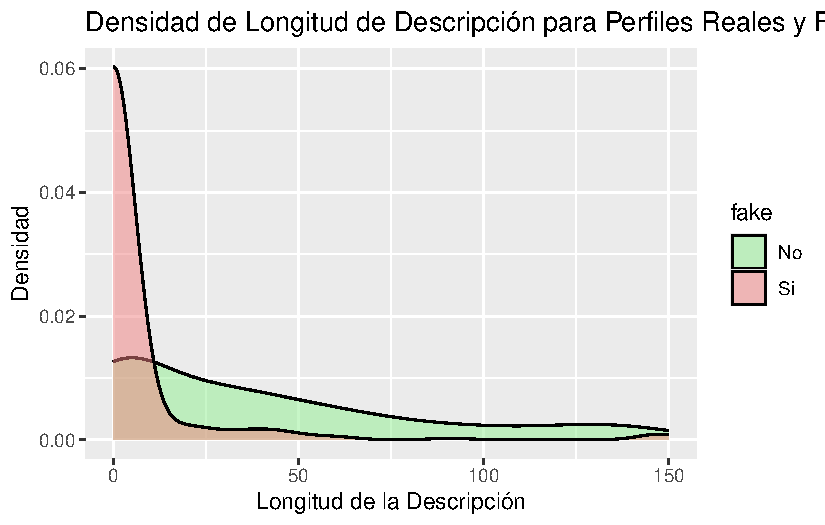
\includegraphics{visualizacionDatos_files/figure-pdf/unnamed-chunk-17-1.pdf}

Y podemos comprobar que dicha idea era cierta, los perfiles falsos
suelen tener un numero reducido de caracteres en su descripción,
mientras que los reales esta mas repartidos.

Vamos a visualizar las medias:

\begin{Shaded}
\begin{Highlighting}[]
\NormalTok{mean\_values }\OtherTok{\textless{}{-}}\NormalTok{ datos\_refinados }\SpecialCharTok{\%\textgreater{}\%} 
  \FunctionTok{group\_by}\NormalTok{(fake) }\SpecialCharTok{\%\textgreater{}\%} 
  \FunctionTok{summarize}\NormalTok{(}\AttributeTok{mean\_desc\_length =} \FunctionTok{mean}\NormalTok{(}\StringTok{\textasciigrave{}}\AttributeTok{description length}\StringTok{\textasciigrave{}}\NormalTok{))}

\FunctionTok{ggplot}\NormalTok{(}\AttributeTok{data =}\NormalTok{ datos\_refinados, }\FunctionTok{aes}\NormalTok{(}\AttributeTok{x =} \StringTok{\textasciigrave{}}\AttributeTok{description length}\StringTok{\textasciigrave{}}\NormalTok{, }\AttributeTok{fill =}\NormalTok{fake)) }\SpecialCharTok{+}
  \FunctionTok{geom\_density}\NormalTok{(}\AttributeTok{alpha =} \FloatTok{0.5}\NormalTok{) }\SpecialCharTok{+}
  \FunctionTok{labs}\NormalTok{(}\AttributeTok{title =} \StringTok{"Densidad de Longitud de Descripción para Perfiles Reales y Falsos"}\NormalTok{,}
       \AttributeTok{x =} \StringTok{"Longitud de la Descripción"}\NormalTok{,}
       \AttributeTok{y =} \StringTok{"Densidad"}\NormalTok{,}
       \AttributeTok{fill =} \StringTok{"Perfil Falso"}\NormalTok{) }\SpecialCharTok{+}
  \FunctionTok{scale\_fill\_manual}\NormalTok{(}\AttributeTok{values =} \FunctionTok{c}\NormalTok{(}\StringTok{"lightgreen"}\NormalTok{, }\StringTok{"lightcoral"}\NormalTok{))}\SpecialCharTok{+}
  \FunctionTok{geom\_vline}\NormalTok{(}\AttributeTok{data =}\NormalTok{ mean\_values, }\FunctionTok{aes}\NormalTok{(}\AttributeTok{xintercept =}\NormalTok{ mean\_desc\_length, }\AttributeTok{color =}\NormalTok{ fake), }\AttributeTok{linetype =} \StringTok{"dashed"}\NormalTok{, }\AttributeTok{size =} \DecValTok{1}\NormalTok{) }\SpecialCharTok{+}
  \FunctionTok{scale\_color\_manual}\NormalTok{(}\AttributeTok{values =} \FunctionTok{c}\NormalTok{(}\StringTok{"lightgreen"}\NormalTok{, }\StringTok{"lightcoral"}\NormalTok{), }\AttributeTok{name =} \StringTok{"Media"}\NormalTok{)}
\end{Highlighting}
\end{Shaded}

\includegraphics{visualizacionDatos_files/figure-pdf/unnamed-chunk-18-1.pdf}

\section{Conclusiones}\label{conclusiones}

Vistos todos los gráficos anteriores, podemos sacar algunas conclusiones
interesantes:

\begin{enumerate}
\def\labelenumi{\arabic{enumi}.}
\item
  Las cuentas falsas tienen menor numero de seguidores y mayor seguidos.
\item
  Las cuentas reales tienen descripciones con longitudes mas largas.
\item
  Las cuentas falsas tiene mas cantidad de caracteres numéricos en el
  nombre completo y nombre de usuario.
\item
  Las cuentas reales siempre suelen tener foto de perfil.
\end{enumerate}

\bookmarksetup{startatroot}

\chapter{Reglas de asociación}\label{reglas-de-asociaciuxf3n}

Vamos a utilizar reglas de asociación para detectar cuentas falsas en
Instagram. Las reglas de asociación son técnicas de minería de datos que
permiten descubrir relaciones interesantes y útiles entre diferentes
características o comportamientos observados en el dataSet.

Para realizar estas operaciones vamos a utilizar el paquete
\texttt{arules.}

\section{Características
importantes}\label{caracteruxedsticas-importantes}

\subsection{Medidas relevantes}\label{medidas-relevantes}

Para evaluar la calidad y relevancia de las reglas de asociación, vamos
a utilizar las medidas de:

\begin{enumerate}
\def\labelenumi{\arabic{enumi}.}
\item
  \textbf{Soporte (Support)}:

  \begin{itemize}
  \item
    El soporte de una regla mide la proporción de cuentas en el dataset
    que contienen ambos conjuntos de características A y B.
  \item
    Un soporte alto indica que la regla se aplica a una gran proporción
    del dataset, lo que sugiere que la combinación de características es
    común y relevante.
  \end{itemize}
\item
  \textbf{Confianza (Confidence)}:

  \begin{itemize}
  \item
    La confianza de una regla mide cuán frecuentemente las
    características en B aparecen en las cuentas que contienen A.
  \item
    A mayor confianza, mayor es la fiabilidad de que la presencia de las
    características en el antecedente de la regla (A) implicará la
    presencia de las características en el consecuente de la regla (B).
  \end{itemize}
\item
  \textbf{Elevación (Lift)}:

  \begin{itemize}
  \item
    La elevación mide la relación entre la aparición conjunta de A y B y
    la aparición esperada de A y B si fueran independientes.
  \item
    Una elevación alta (mayor que 1) indica que la presencia de A
    incrementa significativamente la probabilidad de que B ocurra, lo
    que sugiere una fuerte asociación entre las características.
  \end{itemize}
\end{enumerate}

\subsection{Algoritmo Apriori}\label{algoritmo-apriori}

Vamos a utilizar el algoritmo Apriori como nuestra forma de obtener
reglas a partir de nuestros datos. Este es uno de los algoritmos más
conocidos y se basa en la propiedad de que cualquier subconjunto de un
conjunto frecuente también debe ser frecuente. El algoritmo itera a
través de los conjuntos de características, incrementando su tamaño en
cada iteración y manteniendo solo los conjuntos que cumplen con un
umbral mínimo de soporte.

\subsection{Reglas}\label{reglas}

Las reglas de asociación consisten en implicaciones del tipo ``Si A
entonces B'', donde A y B son conjuntos de características o
comportamientos de las cuentas. Por ejemplo, una regla podría ser ``Si
una cuenta tiene un número alto de cuentas seguidos y no tiene foto de
perfil, entonces es probable que sea una cuenta falsa''.

\section{Cargar datos}\label{cargar-datos}

Vamos a cargar las librería necesarias y nuestro dataSet:

\begin{Shaded}
\begin{Highlighting}[]
\FunctionTok{library}\NormalTok{(arules)}
\end{Highlighting}
\end{Shaded}

\begin{verbatim}
Loading required package: Matrix
\end{verbatim}

\begin{verbatim}

Attaching package: 'arules'
\end{verbatim}

\begin{verbatim}
The following objects are masked from 'package:base':

    abbreviate, write
\end{verbatim}

\begin{Shaded}
\begin{Highlighting}[]
\FunctionTok{library}\NormalTok{(arulesViz)}
\end{Highlighting}
\end{Shaded}

\begin{verbatim}
Warning: package 'arulesViz' was built under R version 4.3.3
\end{verbatim}

\begin{Shaded}
\begin{Highlighting}[]
\FunctionTok{library}\NormalTok{(readr)}
\NormalTok{datos }\OtherTok{\textless{}{-}} \FunctionTok{read\_csv}\NormalTok{(}\StringTok{"Data/train.csv"}\NormalTok{) }
\end{Highlighting}
\end{Shaded}

\begin{verbatim}
Rows: 576 Columns: 12
\end{verbatim}

\begin{verbatim}
-- Column specification --------------------------------------------------------
Delimiter: ","
dbl (12): profile pic, nums/length username, fullname words, nums/length ful...

i Use `spec()` to retrieve the full column specification for this data.
i Specify the column types or set `show_col_types = FALSE` to quiet this message.
\end{verbatim}

\section{Discretizar datos}\label{discretizar-datos}

Puesto que el algoritmo de apriori necesita que el conjunto de datos sea
binario o discreto.

Existen varias formas de discretizar datos, pero el objetivo principal
es convertir las características continuas en valores discretos que
representen de manera efectiva la información subyacente. Algunas
técnicas comunes de discretización incluyen la binarización, la división
en intervalos fijos o basados en cuantiles.

Tras haber realizado el previo análisis exploratorio podemos definir
intervalos personalizados para las cada variable, para ello usaremos las
funciones ordered y cut. Ademas las variables que son binarias como
fake, vamos a ponerle ``Si'' o ``No'' para poder comprenderlo mejor.

\begin{Shaded}
\begin{Highlighting}[]
\NormalTok{datos\_refinados }\OtherTok{\textless{}{-}}\NormalTok{ datos}

\NormalTok{columnas\_binarias }\OtherTok{=} \FunctionTok{c}\NormalTok{(}\StringTok{"profile pic"}\NormalTok{,}\StringTok{"name==username"}\NormalTok{,}\StringTok{"external URL"}\NormalTok{,}\StringTok{"fake"}\NormalTok{,}\StringTok{"private"}\NormalTok{)}

\ControlFlowTok{for}\NormalTok{ (columna }\ControlFlowTok{in}\NormalTok{ columnas\_binarias) \{}
\NormalTok{  datos\_refinados[[columna]] }\OtherTok{\textless{}{-}}  \FunctionTok{factor}\NormalTok{(datos\_refinados[[columna]], }\AttributeTok{labels =} \FunctionTok{c}\NormalTok{(}\StringTok{"No"}\NormalTok{, }\StringTok{"Si"}\NormalTok{))}
\NormalTok{\}}
\end{Highlighting}
\end{Shaded}

\begin{Shaded}
\begin{Highlighting}[]
\CommentTok{\# Discretización de la columna \#posts}
\NormalTok{datos\_refinados}\SpecialCharTok{$}\StringTok{\textasciigrave{}}\AttributeTok{\#posts}\StringTok{\textasciigrave{}} \OtherTok{\textless{}{-}} \FunctionTok{ordered}\NormalTok{(}\FunctionTok{cut}\NormalTok{(datos\_refinados}\SpecialCharTok{$}\StringTok{\textasciigrave{}}\AttributeTok{\#posts}\StringTok{\textasciigrave{}}\NormalTok{, }
                                 \AttributeTok{breaks =} \FunctionTok{c}\NormalTok{(}\DecValTok{0}\NormalTok{,}\DecValTok{1}\NormalTok{, }\DecValTok{5}\NormalTok{, }\DecValTok{10}\NormalTok{, }\DecValTok{50}\NormalTok{, }\ConstantTok{Inf}\NormalTok{), }
                                 \AttributeTok{labels =} \FunctionTok{c}\NormalTok{(}\StringTok{"muy bajo"}\NormalTok{,}\StringTok{"medio"}\NormalTok{, }\StringTok{"alto"}\NormalTok{, }\StringTok{"muy alto"}\NormalTok{, }\StringTok{"extremadamente alto"}\NormalTok{),}\AttributeTok{include.lowest =} \ConstantTok{TRUE}\NormalTok{))}

\CommentTok{\# Discretización de la columna \#followers}
\NormalTok{datos\_refinados}\SpecialCharTok{$}\StringTok{\textasciigrave{}}\AttributeTok{\#followers}\StringTok{\textasciigrave{}} \OtherTok{\textless{}{-}} \FunctionTok{ordered}\NormalTok{(}\FunctionTok{cut}\NormalTok{(datos\_refinados}\SpecialCharTok{$}\StringTok{\textasciigrave{}}\AttributeTok{\#followers}\StringTok{\textasciigrave{}}\NormalTok{, }
                                     \AttributeTok{breaks =} \FunctionTok{c}\NormalTok{(}\DecValTok{0}\NormalTok{, }\DecValTok{10}\NormalTok{, }\DecValTok{60}\NormalTok{, }\DecValTok{200}\NormalTok{, }\ConstantTok{Inf}\NormalTok{), }
                                     \AttributeTok{labels =} \FunctionTok{c}\NormalTok{(}\StringTok{"bajo"}\NormalTok{, }\StringTok{"medio"}\NormalTok{, }\StringTok{"alto"}\NormalTok{, }\StringTok{"muy alto"}\NormalTok{),}\AttributeTok{include.lowest =} \ConstantTok{TRUE}\NormalTok{))}

\CommentTok{\# Discretización de la columna \#follows}
\NormalTok{datos\_refinados}\SpecialCharTok{$}\StringTok{\textasciigrave{}}\AttributeTok{\#follows}\StringTok{\textasciigrave{}} \OtherTok{\textless{}{-}} \FunctionTok{ordered}\NormalTok{(}\FunctionTok{cut}\NormalTok{(datos\_refinados}\SpecialCharTok{$}\StringTok{\textasciigrave{}}\AttributeTok{\#follows}\StringTok{\textasciigrave{}}\NormalTok{, }
                                   \AttributeTok{breaks =} \FunctionTok{c}\NormalTok{(}\DecValTok{0}\NormalTok{, }\DecValTok{10}\NormalTok{, }\DecValTok{60}\NormalTok{, }\DecValTok{200}\NormalTok{, }\ConstantTok{Inf}\NormalTok{), }
                                   \AttributeTok{labels =} \FunctionTok{c}\NormalTok{(}\StringTok{"bajo"}\NormalTok{, }\StringTok{"medio"}\NormalTok{, }\StringTok{"alto"}\NormalTok{, }\StringTok{"muy alto"}\NormalTok{),}\AttributeTok{include.lowest =} \ConstantTok{TRUE}\NormalTok{))}

\CommentTok{\# Discretización de la columna nums/length username}
\NormalTok{datos\_refinados}\SpecialCharTok{$}\StringTok{\textasciigrave{}}\AttributeTok{nums/length username}\StringTok{\textasciigrave{}} \OtherTok{\textless{}{-}} \FunctionTok{ordered}\NormalTok{(}\FunctionTok{cut}\NormalTok{(datos\_refinados}\SpecialCharTok{$}\StringTok{\textasciigrave{}}\AttributeTok{nums/length username}\StringTok{\textasciigrave{}}\NormalTok{,}
                                                      \AttributeTok{breaks =} \FunctionTok{c}\NormalTok{(}\DecValTok{0}\NormalTok{, }\FloatTok{0.2}\NormalTok{, }\FloatTok{0.4}\NormalTok{, }\FloatTok{0.6}\NormalTok{, }\FloatTok{0.8}\NormalTok{, }\DecValTok{1}\NormalTok{),}
                                                      \AttributeTok{labels =} \FunctionTok{c}\NormalTok{(}\StringTok{"muy bajo"}\NormalTok{, }\StringTok{"bajo"}\NormalTok{, }\StringTok{"medio"}\NormalTok{, }\StringTok{"alto"}\NormalTok{, }\StringTok{"muy alto"}\NormalTok{),}
                                                      \AttributeTok{include.lowest =} \ConstantTok{TRUE}\NormalTok{))}

\CommentTok{\# Discretización de la columna nums/length fullname}
\NormalTok{datos\_refinados}\SpecialCharTok{$}\StringTok{\textasciigrave{}}\AttributeTok{nums/length fullname}\StringTok{\textasciigrave{}} \OtherTok{\textless{}{-}} \FunctionTok{ordered}\NormalTok{(}\FunctionTok{cut}\NormalTok{(datos\_refinados}\SpecialCharTok{$}\StringTok{\textasciigrave{}}\AttributeTok{nums/length fullname}\StringTok{\textasciigrave{}}\NormalTok{, }
                                                      \AttributeTok{breaks =} \FunctionTok{c}\NormalTok{(}\DecValTok{0}\NormalTok{, }\FloatTok{0.2}\NormalTok{, }\FloatTok{0.4}\NormalTok{, }\FloatTok{0.6}\NormalTok{, }\FloatTok{0.8}\NormalTok{, }\DecValTok{1}\NormalTok{), }
                                                      \AttributeTok{labels =} \FunctionTok{c}\NormalTok{(}\StringTok{"muy bajo"}\NormalTok{, }\StringTok{"bajo"}\NormalTok{, }\StringTok{"medio"}\NormalTok{, }\StringTok{"alto"}\NormalTok{, }\StringTok{"muy alto"}\NormalTok{),}
                                                      \AttributeTok{include.lowest =} \ConstantTok{TRUE}\NormalTok{))}
\CommentTok{\# Discretización de la columna description length}
\NormalTok{datos\_refinados}\SpecialCharTok{$}\StringTok{\textasciigrave{}}\AttributeTok{description length}\StringTok{\textasciigrave{}} \OtherTok{\textless{}{-}} \FunctionTok{ordered}\NormalTok{(}\FunctionTok{cut}\NormalTok{(datos\_refinados}\SpecialCharTok{$}\StringTok{\textasciigrave{}}\AttributeTok{description length}\StringTok{\textasciigrave{}}\NormalTok{,}
                                                     \AttributeTok{breaks =} \FunctionTok{c}\NormalTok{(}\DecValTok{0}\NormalTok{, }\DecValTok{15}\NormalTok{, }\DecValTok{25}\NormalTok{, }\DecValTok{80}\NormalTok{, }\DecValTok{150}\NormalTok{),}
                                                     \AttributeTok{labels =} \FunctionTok{c}\NormalTok{(}\StringTok{"muy corto"}\NormalTok{ , }\StringTok{"medio"}\NormalTok{, }\StringTok{"largo"}\NormalTok{, }\StringTok{"muy largo"}\NormalTok{),}
                                                    \AttributeTok{include.lowest =} \ConstantTok{TRUE}\NormalTok{))}
\CommentTok{\# Discretización de la columna fullname words}
\NormalTok{datos\_refinados}\SpecialCharTok{$}\StringTok{\textasciigrave{}}\AttributeTok{fullname words}\StringTok{\textasciigrave{}} \OtherTok{\textless{}{-}} \FunctionTok{ordered}\NormalTok{(}\FunctionTok{cut}\NormalTok{(datos\_refinados}\SpecialCharTok{$}\StringTok{\textasciigrave{}}\AttributeTok{fullname words}\StringTok{\textasciigrave{}}\NormalTok{,}
                                                 \AttributeTok{breaks =} \FunctionTok{c}\NormalTok{(}\DecValTok{0}\NormalTok{, }\DecValTok{1}\NormalTok{, }\DecValTok{3}\NormalTok{, }\DecValTok{5}\NormalTok{, }\ConstantTok{Inf}\NormalTok{),}
                                                 \AttributeTok{labels =} \FunctionTok{c}\NormalTok{(}\StringTok{"muy corto"}\NormalTok{, }\StringTok{"medio"}\NormalTok{, }\StringTok{"largo"}\NormalTok{, }\StringTok{"muy largo"}\NormalTok{),}\AttributeTok{include.lowest =} \ConstantTok{TRUE}\NormalTok{))}
\end{Highlighting}
\end{Shaded}

\subsection{discretizeDF}\label{discretizedf}

Esta función del paquete de arules implementa varios métodos básicos no
supervisados para convertir una variable continua en una variable
categórica (factor) usando diferentes estrategias de agrupamiento.

Vamos a quitar primero las columnas binarias que le queremos poner un
valor custom.

\begin{Shaded}
\begin{Highlighting}[]
\NormalTok{datos\_refinados\_clone }\OtherTok{\textless{}{-}}\NormalTok{ datos}

\NormalTok{columnas\_binarias }\OtherTok{=} \FunctionTok{c}\NormalTok{(}\StringTok{"profile pic"}\NormalTok{,}\StringTok{"name==username"}\NormalTok{,}\StringTok{"external URL"}\NormalTok{,}\StringTok{"fake"}\NormalTok{,}\StringTok{"private"}\NormalTok{)}

\ControlFlowTok{for}\NormalTok{ (columna }\ControlFlowTok{in}\NormalTok{ columnas\_binarias) \{}
\NormalTok{  datos\_refinados\_clone[[columna]] }\OtherTok{\textless{}{-}}  \FunctionTok{factor}\NormalTok{(datos\_refinados\_clone[[columna]], }\AttributeTok{labels =} \FunctionTok{c}\NormalTok{(}\StringTok{"No"}\NormalTok{, }\StringTok{"Si"}\NormalTok{))}
\NormalTok{\}}
\end{Highlighting}
\end{Shaded}

Vamos a ver algunas estrategias:

\subsubsection{K-means:}\label{k-means}

\begin{Shaded}
\begin{Highlighting}[]
\NormalTok{kmeansDisc }\OtherTok{\textless{}{-}} \FunctionTok{discretizeDF}\NormalTok{(datos\_refinados\_clone, }\AttributeTok{default =} \FunctionTok{list}\NormalTok{(}\AttributeTok{method =} \StringTok{"cluster"}\NormalTok{, }\AttributeTok{breaks =} \DecValTok{5}\NormalTok{, }
  \AttributeTok{labels =} \FunctionTok{c}\NormalTok{(}\StringTok{"muy bajo"}\NormalTok{, }\StringTok{"bajo"}\NormalTok{,}\StringTok{"medio"}\NormalTok{,}\StringTok{"alto"}\NormalTok{,}\StringTok{"muy alto"}\NormalTok{)))}
\FunctionTok{head}\NormalTok{(kmeansDisc)}
\end{Highlighting}
\end{Shaded}

\begin{verbatim}
# A tibble: 6 x 12
  `profile pic` `nums/length username` `fullname words` `nums/length fullname`
  <fct>         <fct>                  <fct>            <fct>                 
1 Si            bajo                   muy bajo         muy bajo              
2 Si            muy bajo               bajo             muy bajo              
3 Si            muy bajo               bajo             muy bajo              
4 Si            muy bajo               bajo             muy bajo              
5 Si            muy bajo               bajo             muy bajo              
6 Si            muy bajo               medio            muy bajo              
# i 8 more variables: `name==username` <fct>, `description length` <fct>,
#   `external URL` <fct>, private <fct>, `#posts` <fct>, `#followers` <fct>,
#   `#follows` <fct>, fake <fct>
\end{verbatim}

\subsubsection{interval}\label{interval}

\begin{Shaded}
\begin{Highlighting}[]
\NormalTok{fixedDisc }\OtherTok{\textless{}{-}} \FunctionTok{discretizeDF}\NormalTok{(datos\_refinados\_clone, }\AttributeTok{default =} \FunctionTok{list}\NormalTok{(}\AttributeTok{method =} \StringTok{"interval"}\NormalTok{, }\AttributeTok{breaks =} \DecValTok{5}\NormalTok{, }
  \AttributeTok{labels =} \FunctionTok{c}\NormalTok{(}\StringTok{"muy bajo"}\NormalTok{, }\StringTok{"bajo"}\NormalTok{,}\StringTok{"medio"}\NormalTok{,}\StringTok{"alto"}\NormalTok{,}\StringTok{"muy alto"}\NormalTok{)))}
\FunctionTok{head}\NormalTok{(fixedDisc)}
\end{Highlighting}
\end{Shaded}

\begin{verbatim}
# A tibble: 6 x 12
  `profile pic` `nums/length username` `fullname words` `nums/length fullname`
  <fct>         <fct>                  <fct>            <fct>                 
1 Si            bajo                   muy bajo         muy bajo              
2 Si            muy bajo               muy bajo         muy bajo              
3 Si            muy bajo               muy bajo         muy bajo              
4 Si            muy bajo               muy bajo         muy bajo              
5 Si            muy bajo               muy bajo         muy bajo              
6 Si            muy bajo               bajo             muy bajo              
# i 8 more variables: `name==username` <fct>, `description length` <fct>,
#   `external URL` <fct>, private <fct>, `#posts` <fct>, `#followers` <fct>,
#   `#follows` <fct>, fake <fct>
\end{verbatim}

\section{Generar dataset de
transacciones}\label{generar-dataset-de-transacciones}

Ahora una vez discretizado el dataframe, el siguiente paso es generar un
dataset de transacciones. Este tipo de dataset es esencial para aplicar
algoritmos de reglas de asociación como Apriori.

En un dataset de transacciones, cada fila representa una transacción,
que es una colección de elementos o ítems.

\begin{Shaded}
\begin{Highlighting}[]
\NormalTok{datos\_refinadosT }\OtherTok{\textless{}{-}} \FunctionTok{as}\NormalTok{(datos\_refinados, }\StringTok{"transactions"}\NormalTok{)}
\end{Highlighting}
\end{Shaded}

\section{Generar reglas}\label{generar-reglas}

Ahora que ya tenemos todo listo, podemos utilizar los algoritmos de
generacion de reglas. En nuestro caso, vamos a utilizar apriori. Para
generar reglas primero necesitamos establecer un valor para el suport y
confianza minima, estos valores nos permitirán controlar la cantidad y
calidad de las reglas que se generarán.

\begin{Shaded}
\begin{Highlighting}[]
\NormalTok{ rules }\OtherTok{\textless{}{-}} \FunctionTok{apriori}\NormalTok{(datos\_refinadosT,  }\AttributeTok{parameter =} \FunctionTok{list}\NormalTok{(}\AttributeTok{supp =} \FloatTok{0.3}\NormalTok{, }\AttributeTok{conf =} \FloatTok{0.01}\NormalTok{, }\AttributeTok{target =} \StringTok{"rules"}\NormalTok{)) }
\end{Highlighting}
\end{Shaded}

\begin{verbatim}
Apriori

Parameter specification:
 confidence minval smax arem  aval originalSupport maxtime support minlen
       0.01    0.1    1 none FALSE            TRUE       5     0.3      1
 maxlen target  ext
     10  rules TRUE

Algorithmic control:
 filter tree heap memopt load sort verbose
    0.1 TRUE TRUE  FALSE TRUE    2    TRUE

Absolute minimum support count: 172 

set item appearances ...[0 item(s)] done [0.00s].
set transactions ...[40 item(s), 576 transaction(s)] done [0.00s].
sorting and recoding items ... [16 item(s)] done [0.00s].
creating transaction tree ... done [0.00s].
checking subsets of size 1 2 3 4 5 6 7 done [0.00s].
writing ... [1157 rule(s)] done [0.00s].
creating S4 object  ... done [0.00s].
\end{verbatim}

\begin{Shaded}
\begin{Highlighting}[]
\NormalTok{ rules}
\end{Highlighting}
\end{Shaded}

\begin{verbatim}
set of 1157 rules 
\end{verbatim}

Hemos obtenido una buena cantidad de reglas para continuar nuestro
análisis.

\section{Refinar reglas}\label{refinar-reglas}

Ahora que hemos obtenido las reglas necesitamos cribarlarlas y eliminar
todas aquellas que no nos interesan, que sean redundantes o no
significativas.

\subsection{Eliminar reglas
redundantes}\label{eliminar-reglas-redundantes}

\begin{Shaded}
\begin{Highlighting}[]
\NormalTok{rules }\OtherTok{\textless{}{-}}\NormalTok{ rules[}\FunctionTok{which}\NormalTok{(}\FunctionTok{is.redundant}\NormalTok{(rules))]}
\end{Highlighting}
\end{Shaded}

\subsection{Eliminar reglas no
significativas}\label{eliminar-reglas-no-significativas}

\begin{Shaded}
\begin{Highlighting}[]
\NormalTok{rules }\OtherTok{\textless{}{-}}\NormalTok{ rules[}\FunctionTok{which}\NormalTok{(}\FunctionTok{is.significant}\NormalTok{(rules))]}
\end{Highlighting}
\end{Shaded}

Vamos a ver cuentas reglas han quedado después de filtrarlas:

\begin{Shaded}
\begin{Highlighting}[]
\FunctionTok{length}\NormalTok{(rules)}
\end{Highlighting}
\end{Shaded}

\begin{verbatim}
[1] 569
\end{verbatim}

\section{Análisis de reglas
obtenidas}\label{anuxe1lisis-de-reglas-obtenidas}

Nuestro objetivo es detectar y diferenciar cuentas falses de las
verdaderas, por lo tanto, vamos a centrar nuestro analisis en eso dos
atributos ``fake=Si'' y ``fake=No''. Como tenemos diferentes metricas,
vamos a analizarlas por separado:

\subsection{Support:}\label{support}

Vamos priemro a analizar las reglas ordenando primero por el soporte de
la reglas. Recordamos que el soporte alto indica que la regla se aplica
a una gran proporción del dataset, lo que sugiere que la combinación de
características es común y relevante.

\begin{Shaded}
\begin{Highlighting}[]
\NormalTok{rules }\OtherTok{\textless{}{-}} \FunctionTok{sort}\NormalTok{(rules,}\AttributeTok{by=}\StringTok{"support"}\NormalTok{)}
\FunctionTok{inspect}\NormalTok{(}\FunctionTok{head}\NormalTok{(rules))}
\end{Highlighting}
\end{Shaded}

\begin{verbatim}
    lhs                                 rhs                               support confidence  coverage     lift count
[1] {nums/length fullname=muy bajo,                                                                                  
     external URL=No}                => {name==username=No}             0.7881944  0.9848156 0.8003472 1.020241   454
[2] {nums/length username=muy bajo,                                                                                  
     name==username=No}              => {nums/length fullname=muy bajo} 0.6250000  0.9863014 0.6336806 1.078007   360
[3] {nums/length fullname=muy bajo,                                                                                  
     name==username=No}              => {nums/length username=muy bajo} 0.6250000  0.6936416 0.9010417 1.071146   360
[4] {name==username=No,                                                                                              
     description length=muy corto}   => {external URL=No}               0.6041667  0.9747899 0.6197917 1.103102   348
[5] {name==username=No,                                                                                              
     external URL=No}                => {description length=muy corto}  0.6041667  0.7102041 0.8506944 1.096723   348
[6] {nums/length fullname=muy bajo,                                                                                  
     description length=muy corto}   => {external URL=No}               0.5590278  0.9728097 0.5746528 1.100861   322
\end{verbatim}

En este caso, el soporte es 0.7881944, lo que significa que el 78.82\%
de las transacciones en el dataset contienen tanto el antecedente
\{nums/length fullname=muy bajo, external URL=No\} como el consecuente
\{name==username=No\}.

\begin{Shaded}
\begin{Highlighting}[]
\NormalTok{r2 }\OtherTok{\textless{}{-}} \FunctionTok{subset}\NormalTok{(rules, }\AttributeTok{subset =}\NormalTok{ rhs }\SpecialCharTok{\%in\%} \FunctionTok{c}\NormalTok{(}\StringTok{"fake=Si"}\NormalTok{))}
\FunctionTok{inspect}\NormalTok{(}\FunctionTok{head}\NormalTok{(r2))}
\end{Highlighting}
\end{Shaded}

\begin{verbatim}
    lhs                                 rhs         support confidence  coverage     lift count
[1] {name==username=No,                                                                        
     external URL=No}                => {fake=Si} 0.4670139  0.5489796 0.8506944 1.097959   269
[2] {name==username=No,                                                                        
     description length=muy corto}   => {fake=Si} 0.4253472  0.6862745 0.6197917 1.372549   245
[3] {name==username=No,                                                                        
     description length=muy corto,                                                             
     external URL=No}                => {fake=Si} 0.4253472  0.7040230 0.6041667 1.408046   245
[4] {nums/length fullname=muy bajo,                                                            
     external URL=No}                => {fake=Si} 0.4218750  0.5271150 0.8003472 1.054230   243
[5] {nums/length fullname=muy bajo,                                                            
     description length=muy corto}   => {fake=Si} 0.3819444  0.6646526 0.5746528 1.329305   220
[6] {nums/length fullname=muy bajo,                                                            
     description length=muy corto,                                                             
     external URL=No}                => {fake=Si} 0.3819444  0.6832298 0.5590278 1.366460   220
\end{verbatim}

\subsection{Confianza:}\label{confianza}

Ahora va a analizar las reglas ordenando por la confianza en la reglas.
Recordamos que a mayor confianza, mayor es la fiabilidad de que la
presencia de las características en el antecedente de la regla A
implicará la presencia de las características en el consecuente de la
regla B.

\begin{Shaded}
\begin{Highlighting}[]
\NormalTok{rules }\OtherTok{\textless{}{-}} \FunctionTok{sort}\NormalTok{(rules,}\AttributeTok{by=}\StringTok{"confidence"}\NormalTok{)}
\FunctionTok{inspect}\NormalTok{(}\FunctionTok{head}\NormalTok{(rules)) }
\end{Highlighting}
\end{Shaded}

\begin{verbatim}
    lhs                                 rhs                   support confidence  coverage     lift count
[1] {name==username=No,                                                                                  
     fake=Si}                        => {external URL=No}   0.4670139          1 0.4670139 1.131631   269
[2] {description length=muy corto,                                                                       
     fake=Si}                        => {external URL=No}   0.4531250          1 0.4531250 1.131631   261
[3] {name==username=No,                                                                                  
     description length=muy corto,                                                                       
     fake=Si}                        => {external URL=No}   0.4253472          1 0.4253472 1.131631   245
[4] {nums/length fullname=muy bajo,                                                                      
     fake=Si}                        => {external URL=No}   0.4218750          1 0.4218750 1.131631   243
[5] {profile pic=Si,                                                                                     
     nums/length fullname=muy bajo,                                                                      
     #followers=muy alto}            => {name==username=No} 0.4166667          1 0.4166667 1.035971   240
[6] {nums/length fullname=muy bajo,                                                                      
     name==username=No,                                                                                  
     fake=Si}                        => {external URL=No}   0.4097222          1 0.4097222 1.131631   236
\end{verbatim}

En este caso, la confianza es 1, lo que significa que el 100\% de las
transacciones que tienen el antecedente también tienen el consecuente.

\begin{Shaded}
\begin{Highlighting}[]
\NormalTok{r2 }\OtherTok{\textless{}{-}} \FunctionTok{subset}\NormalTok{(rules, }\AttributeTok{subset =}\NormalTok{ rhs }\SpecialCharTok{\%in\%} \FunctionTok{c}\NormalTok{(}\StringTok{"fake=Si"}\NormalTok{))}
\FunctionTok{inspect}\NormalTok{(}\FunctionTok{head}\NormalTok{(r2))}
\end{Highlighting}
\end{Shaded}

\begin{verbatim}
    lhs                                 rhs         support confidence  coverage     lift count
[1] {external URL=No,                                                                          
     #posts=muy bajo}                => {fake=Si} 0.3072917  0.9567568 0.3211806 1.913514   177
[2] {fullname words=muy corto,                                                                 
     name==username=No,                                                                        
     description length=muy corto,                                                             
     external URL=No}                => {fake=Si} 0.3454861  0.8122449 0.4253472 1.624490   199
[3] {fullname words=muy corto,                                                                 
     name==username=No,                                                                        
     description length=muy corto}   => {fake=Si} 0.3454861  0.8024194 0.4305556 1.604839   199
[4] {fullname words=muy corto,                                                                 
     nums/length fullname=muy bajo,                                                            
     description length=muy corto,                                                             
     external URL=No}                => {fake=Si} 0.3072917  0.7972973 0.3854167 1.594595   177
[5] {fullname words=muy corto,                                                                 
     nums/length fullname=muy bajo,                                                            
     description length=muy corto}   => {fake=Si} 0.3072917  0.7866667 0.3906250 1.573333   177
[6] {fullname words=muy corto,                                                                 
     name==username=No,                                                                        
     external URL=No}                => {fake=Si} 0.3750000  0.7105263 0.5277778 1.421053   216
\end{verbatim}

\subsection{Lift:}\label{lift}

Por ultimo, vamos a analizar las reglas ordenando primero por el lift de
la reglas. Recordamos que un lift alto indica que la presencia de A
incrementa significativamente la probabilidad de que B ocurra, lo que
sugiere una fuerte asociación entre las características.

\begin{Shaded}
\begin{Highlighting}[]
\NormalTok{rules }\OtherTok{\textless{}{-}} \FunctionTok{sort}\NormalTok{(rules,}\AttributeTok{by=}\StringTok{"lift"}\NormalTok{)}
\FunctionTok{inspect}\NormalTok{(}\FunctionTok{head}\NormalTok{(rules)) }
\end{Highlighting}
\end{Shaded}

\begin{verbatim}
    lhs                                 rhs                     support confidence  coverage     lift count
[1] {name==username=No,                                                                                    
     #follows=muy alto,                                                                                    
     fake=No}                        => {#followers=muy alto} 0.3506944  0.9223744 0.3802083 2.059255   202
[2] {profile pic=Si,                                                                                       
     #follows=muy alto,                                                                                    
     fake=No}                        => {#followers=muy alto} 0.3472222  0.9216590 0.3767361 2.057657   200
[3] {profile pic=Si,                                                                                       
     name==username=No,                                                                                    
     #follows=muy alto,                                                                                    
     fake=No}                        => {#followers=muy alto} 0.3472222  0.9216590 0.3767361 2.057657   200
[4] {nums/length fullname=muy bajo,                                                                        
     #follows=muy alto,                                                                                    
     fake=No}                        => {#followers=muy alto} 0.3437500  0.9209302 0.3732639 2.056030   198
[5] {nums/length fullname=muy bajo,                                                                        
     name==username=No,                                                                                    
     #follows=muy alto,                                                                                    
     fake=No}                        => {#followers=muy alto} 0.3437500  0.9209302 0.3732639 2.056030   198
[6] {nums/length username=muy bajo,                                                                        
     #follows=muy alto,                                                                                    
     fake=No}                        => {#followers=muy alto} 0.3229167  0.9207921 0.3506944 2.055722   186
\end{verbatim}

En este caso, el lift es 5.731343, lo que sugiere que la aparicion de
``external URL=Si'' es aproximadamente 5.73 veces más probable cuando se
dan las condiciones en el antecedente.

\begin{Shaded}
\begin{Highlighting}[]
\NormalTok{r2 }\OtherTok{\textless{}{-}} \FunctionTok{subset}\NormalTok{(rules, }\AttributeTok{subset =}\NormalTok{ rhs }\SpecialCharTok{\%in\%} \FunctionTok{c}\NormalTok{(}\StringTok{"fake=Si"}\NormalTok{)) }
\FunctionTok{inspect}\NormalTok{(}\FunctionTok{head}\NormalTok{(r2))}
\end{Highlighting}
\end{Shaded}

\begin{verbatim}
    lhs                                 rhs         support confidence  coverage     lift count
[1] {external URL=No,                                                                          
     #posts=muy bajo}                => {fake=Si} 0.3072917  0.9567568 0.3211806 1.913514   177
[2] {fullname words=muy corto,                                                                 
     name==username=No,                                                                        
     description length=muy corto,                                                             
     external URL=No}                => {fake=Si} 0.3454861  0.8122449 0.4253472 1.624490   199
[3] {fullname words=muy corto,                                                                 
     name==username=No,                                                                        
     description length=muy corto}   => {fake=Si} 0.3454861  0.8024194 0.4305556 1.604839   199
[4] {fullname words=muy corto,                                                                 
     nums/length fullname=muy bajo,                                                            
     description length=muy corto,                                                             
     external URL=No}                => {fake=Si} 0.3072917  0.7972973 0.3854167 1.594595   177
[5] {fullname words=muy corto,                                                                 
     nums/length fullname=muy bajo,                                                            
     description length=muy corto}   => {fake=Si} 0.3072917  0.7866667 0.3906250 1.573333   177
[6] {fullname words=muy corto,                                                                 
     name==username=No,                                                                        
     external URL=No}                => {fake=Si} 0.3750000  0.7105263 0.5277778 1.421053   216
\end{verbatim}

\section{}\label{section}

\section{Visualizacion de reglas}\label{visualizacion-de-reglas}

\begin{Shaded}
\begin{Highlighting}[]
\FunctionTok{plot}\NormalTok{(rules)}
\end{Highlighting}
\end{Shaded}

\begin{verbatim}
To reduce overplotting, jitter is added! Use jitter = 0 to prevent jitter.
\end{verbatim}

\includegraphics{reglasAsociacion_files/figure-pdf/unnamed-chunk-18-1.pdf}

\bookmarksetup{startatroot}

\chapter{Formal Concept Analysis}\label{formal-concept-analysis}

El Formal Concept Analysis, o FCA, es una técnica de análisis de datos
originada en la teoría de conjuntos formales, la lógica matemática y la
teoría de retículos. Su objetivo principal es descubrir y representar
estructuras conceptuales dentro de conjuntos de datos, especialmente
conjuntos de datos que contienen información de tipo jerárquico o
taxonómico.

Las pricipales aplicaiciones de FCA son la extracción de conocimiento,
agrupamiento y clasificación, aprendizaje automático, conceptos,
ontologías, reglas, reglas de asociación, implicaciones de atributos.

Para el FCA, nuestros datos se dividen en objetos y atributos. En
nuestro dataSet, los objetos son las cuentas de usuario y los atributos
son las culumnas como ``Tiene foto de perfil, No tes fake, \ldots.''.

\begin{Shaded}
\begin{Highlighting}[]
\FunctionTok{library}\NormalTok{(fcaR)}
\end{Highlighting}
\end{Shaded}

\begin{verbatim}
Warning: package 'fcaR' was built under R version 4.3.3
\end{verbatim}

\begin{Shaded}
\begin{Highlighting}[]
\FunctionTok{library}\NormalTok{(readr)}
\NormalTok{datos }\OtherTok{\textless{}{-}} \FunctionTok{read\_csv}\NormalTok{(}\StringTok{"Data/train.csv"}\NormalTok{) }
\end{Highlighting}
\end{Shaded}

\begin{verbatim}
Rows: 576 Columns: 12
-- Column specification --------------------------------------------------------
Delimiter: ","
dbl (12): profile pic, nums/length username, fullname words, nums/length ful...

i Use `spec()` to retrieve the full column specification for this data.
i Specify the column types or set `show_col_types = FALSE` to quiet this message.
\end{verbatim}

\begin{Shaded}
\begin{Highlighting}[]
\NormalTok{datos\_refinados }\OtherTok{\textless{}{-}}\NormalTok{ datos}

\NormalTok{columnas\_binarias }\OtherTok{=} \FunctionTok{c}\NormalTok{(}\StringTok{"profile pic"}\NormalTok{,}\StringTok{"name==username"}\NormalTok{,}\StringTok{"external URL"}\NormalTok{,}\StringTok{"fake"}\NormalTok{,}\StringTok{"private"}\NormalTok{)}

\ControlFlowTok{for}\NormalTok{ (columna }\ControlFlowTok{in}\NormalTok{ columnas\_binarias) \{}
\NormalTok{  datos\_refinados[[columna]] }\OtherTok{\textless{}{-}}  \FunctionTok{factor}\NormalTok{(datos\_refinados[[columna]], }\AttributeTok{labels =} \FunctionTok{c}\NormalTok{(}\StringTok{"No"}\NormalTok{, }\StringTok{"Si"}\NormalTok{))}
\NormalTok{\}}

\NormalTok{fc\_datos }\OtherTok{\textless{}{-}}\NormalTok{ FormalContext}\SpecialCharTok{$}\FunctionTok{new}\NormalTok{(datos\_refinados)}
\NormalTok{fc\_datos}
\end{Highlighting}
\end{Shaded}

\begin{verbatim}
FormalContext with 576 objects and 12 attributes.
# A tibble: 576 x 12
   `profile pic` `nums/length username` `fullname words` `nums/length fullname`
   <fct>                          <dbl>            <dbl>                  <dbl>
 1 Si                              0.27                0                      0
 2 Si                              0                   2                      0
 3 Si                              0.1                 2                      0
 4 Si                              0                   1                      0
 5 Si                              0                   2                      0
 6 Si                              0                   4                      0
 7 Si                              0                   2                      0
 8 Si                              0                   2                      0
 9 Si                              0                   0                      0
10 Si                              0                   2                      0
# i 566 more rows
# i 8 more variables: `name==username` <fct>, `description length` <dbl>,
#   `external URL` <fct>, private <fct>, `#posts` <dbl>, `#followers` <dbl>,
#   `#follows` <dbl>, fake <fct>
\end{verbatim}

\section{Escalado}\label{escalado}

Como necesitamos que nuestro dataSet sea binario, necesitamos aplicarles
tecniac como el escaldo para obtener el resultado deseado:

\subsection{Escalado nominal}\label{escalado-nominal}

El escalado nominal se utiliza para atributos cuyos valores son
excluyentes el uno del otro, como por ejemplo, los atributos que son Si
y No.

\begin{Shaded}
\begin{Highlighting}[]
\NormalTok{fc\_datos}\SpecialCharTok{$}\FunctionTok{scale}\NormalTok{(}\StringTok{"profile pic"}\NormalTok{,}\AttributeTok{type =} \StringTok{"nominal"}\NormalTok{,}\FunctionTok{c}\NormalTok{(}\StringTok{"Si"}\NormalTok{,}\StringTok{"No"}\NormalTok{))}
\NormalTok{fc\_datos}\SpecialCharTok{$}\FunctionTok{scale}\NormalTok{(}\StringTok{"name==username"}\NormalTok{,}\AttributeTok{type =} \StringTok{"nominal"}\NormalTok{,}\FunctionTok{c}\NormalTok{(}\StringTok{"Si"}\NormalTok{,}\StringTok{"No"}\NormalTok{))}
\NormalTok{fc\_datos}\SpecialCharTok{$}\FunctionTok{scale}\NormalTok{(}\StringTok{"fake"}\NormalTok{,}\AttributeTok{type =} \StringTok{"nominal"}\NormalTok{,}\FunctionTok{c}\NormalTok{(}\StringTok{"Si"}\NormalTok{,}\StringTok{"No"}\NormalTok{))}
\NormalTok{fc\_datos}\SpecialCharTok{$}\FunctionTok{scale}\NormalTok{(}\StringTok{"private"}\NormalTok{,}\AttributeTok{type =} \StringTok{"nominal"}\NormalTok{,}\FunctionTok{c}\NormalTok{(}\StringTok{"Si"}\NormalTok{,}\StringTok{"No"}\NormalTok{))}
\NormalTok{fc\_datos}\SpecialCharTok{$}\FunctionTok{scale}\NormalTok{(}\StringTok{"external URL"}\NormalTok{,}\AttributeTok{type =} \StringTok{"nominal"}\NormalTok{,}\FunctionTok{c}\NormalTok{(}\StringTok{"Si"}\NormalTok{,}\StringTok{"No"}\NormalTok{))}
\NormalTok{fc\_datos}
\end{Highlighting}
\end{Shaded}

\begin{verbatim}
FormalContext with 576 objects and 17 attributes.
# A tibble: 576 x 17
   `profile pic = Si` `profile pic = No` `nums/length username` `fullname words`
                <dbl>              <dbl>                  <dbl>            <dbl>
 1                  1                  0                   0.27                0
 2                  1                  0                   0                   2
 3                  1                  0                   0.1                 2
 4                  1                  0                   0                   1
 5                  1                  0                   0                   2
 6                  1                  0                   0                   4
 7                  1                  0                   0                   2
 8                  1                  0                   0                   2
 9                  1                  0                   0                   0
10                  1                  0                   0                   2
# i 566 more rows
# i 13 more variables: `nums/length fullname` <dbl>,
#   `name==username = Si` <dbl>, `name==username = No` <dbl>,
#   `description length` <dbl>, `external URL = Si` <dbl>,
#   `external URL = No` <dbl>, `private = Si` <dbl>, `private = No` <dbl>,
#   `#posts` <dbl>, `#followers` <dbl>, `#follows` <dbl>, `fake = Si` <dbl>,
#   `fake = No` <dbl>
\end{verbatim}

\subsection{Escalado intervalos}\label{escalado-intervalos}

Como los demás datos son valores continuos, tenemos que utilizar un tipo
de escalado distinto. Podemos utilizar modos como el ordinal, sin
embargo, este nos generaría conceptos demasiados largos, por lo que el
mejor modo a emplear para estos datos es el intervalo.

\begin{Shaded}
\begin{Highlighting}[]
\NormalTok{fc\_datos}\SpecialCharTok{$}\FunctionTok{scale}\NormalTok{(}\StringTok{"nums/length username"}\NormalTok{, }
         \AttributeTok{type =} \StringTok{"interval"}\NormalTok{, }
         \AttributeTok{values =}\FunctionTok{c}\NormalTok{(}\DecValTok{0}\NormalTok{, }\FloatTok{0.2}\NormalTok{, }\FloatTok{0.4}\NormalTok{, }\FloatTok{0.6}\NormalTok{, }\FloatTok{0.8}\NormalTok{, }\DecValTok{1}\NormalTok{)}
\NormalTok{         )}

\NormalTok{fc\_datos}\SpecialCharTok{$}\FunctionTok{scale}\NormalTok{(}\StringTok{"nums/length fullname"}\NormalTok{, }
         \AttributeTok{type =} \StringTok{"interval"}\NormalTok{, }
         \AttributeTok{values =} \FunctionTok{c}\NormalTok{(}\DecValTok{0}\NormalTok{, }\FloatTok{0.2}\NormalTok{, }\FloatTok{0.4}\NormalTok{, }\FloatTok{0.6}\NormalTok{, }\FloatTok{0.8}\NormalTok{, }\DecValTok{1}\NormalTok{) }
\NormalTok{        )}

\NormalTok{fc\_datos}\SpecialCharTok{$}\FunctionTok{scale}\NormalTok{(}\StringTok{"fullname words"}\NormalTok{, }
         \AttributeTok{type =} \StringTok{"interval"}\NormalTok{, }
         \AttributeTok{values =} \FunctionTok{c}\NormalTok{(}\DecValTok{0}\NormalTok{, }\DecValTok{1}\NormalTok{, }\DecValTok{3}\NormalTok{, }\DecValTok{5}\NormalTok{, }\ConstantTok{Inf}\NormalTok{) }
\NormalTok{         )}

\NormalTok{fc\_datos}\SpecialCharTok{$}\FunctionTok{scale}\NormalTok{(}\StringTok{"description length"}\NormalTok{, }
         \AttributeTok{type =} \StringTok{"interval"}\NormalTok{, }
         \AttributeTok{values =}\FunctionTok{c}\NormalTok{(}\DecValTok{0}\NormalTok{, }\DecValTok{15}\NormalTok{, }\DecValTok{25}\NormalTok{, }\DecValTok{80}\NormalTok{, }\DecValTok{150}\NormalTok{)}
\NormalTok{         )}

\NormalTok{fc\_datos}\SpecialCharTok{$}\FunctionTok{scale}\NormalTok{(}\StringTok{"\#posts"}\NormalTok{, }
         \AttributeTok{type =} \StringTok{"interval"}\NormalTok{, }
         \AttributeTok{values =}  \FunctionTok{c}\NormalTok{(}\DecValTok{0}\NormalTok{,}\DecValTok{1}\NormalTok{, }\DecValTok{5}\NormalTok{, }\DecValTok{10}\NormalTok{, }\DecValTok{50}\NormalTok{, }\ConstantTok{Inf}\NormalTok{)}
\NormalTok{         )}

\NormalTok{fc\_datos}\SpecialCharTok{$}\FunctionTok{scale}\NormalTok{(}\StringTok{"\#followers"}\NormalTok{, }
         \AttributeTok{type =} \StringTok{"interval"}\NormalTok{, }
         \AttributeTok{values =} \FunctionTok{c}\NormalTok{(}\DecValTok{0}\NormalTok{, }\DecValTok{10}\NormalTok{, }\DecValTok{60}\NormalTok{, }\DecValTok{200}\NormalTok{, }\ConstantTok{Inf}\NormalTok{)}
\NormalTok{         )}

\NormalTok{fc\_datos}\SpecialCharTok{$}\FunctionTok{scale}\NormalTok{(}\StringTok{"\#follows"}\NormalTok{, }
         \AttributeTok{type =} \StringTok{"interval"}\NormalTok{, }
         \AttributeTok{values =} \FunctionTok{c}\NormalTok{(}\DecValTok{0}\NormalTok{, }\DecValTok{10}\NormalTok{, }\DecValTok{60}\NormalTok{, }\DecValTok{200}\NormalTok{, }\ConstantTok{Inf}\NormalTok{)}
\NormalTok{         )}
\end{Highlighting}
\end{Shaded}

\section{Conceptos}\label{conceptos}

Una vez tenemos los datos en la forma que buscamos, podemos utilizar el
paquete fcaR para generar conceptos.Los conceptos son componentes
fundamentales que representan agrupaciones de objetos y atributos con
una relación particular.

De manera formal, un concepto (𝐴,𝐵) se define como un par donde:

\begin{itemize}
\item
  𝐴 es el conjunto de objetos (extensión) que tienen todos los atributos
  de 𝐵.
\item
  𝐵 es el conjunto de atributos (intensión) que son poseídos por todos
  los objetos de 𝐴.
\end{itemize}

\subsection{Calculo de los conceptos del
contexto}\label{calculo-de-los-conceptos-del-contexto}

Para calcular los conceptos de nuestros datos utilizamos la función
\texttt{find\_concepts}

\begin{Shaded}
\begin{Highlighting}[]
\NormalTok{fc\_datos}\SpecialCharTok{$}\FunctionTok{find\_concepts}\NormalTok{()}

\NormalTok{fc\_datos}\SpecialCharTok{$}\NormalTok{concepts}\SpecialCharTok{$}\FunctionTok{size}\NormalTok{()}
\end{Highlighting}
\end{Shaded}

\begin{verbatim}
[1] 7008
\end{verbatim}

Vemos que hemos obtenido un gran numero de conceptos, vamos a ver los
primeros:

\begin{Shaded}
\begin{Highlighting}[]
\FunctionTok{head}\NormalTok{(fc\_datos}\SpecialCharTok{$}\NormalTok{concepts)}
\end{Highlighting}
\end{Shaded}

\begin{verbatim}
A set of 6 concepts:
1: ({1, 2, 3, 4, 5, 6, 7, 8, 9, 10, 11, 12, 13, 14, 15, 16, 17, 18, 19, 20, 21, 22, 23, 24, 25, 26, 27, 28, 29, 30, 31, 32, 33, 34, 35, 36, 37, 38, 39, 40, 41, 42, 43, 44, 45, 46, 47, 48, 49, 50, 51, 52, 53, 54, 55, 56, 57, 58, 59, 60, 61, 62, 63, 64, 65, 66, 67, 68, 69, 70, 71, 72, 73, 74, 75, 76, 77, 78, 79, 80, 81, 82, 83, 84, 85, 86, 87, 88, 89, 90, 91, 92, 93, 94, 95, 96, 97, 98, 99, 100, 101, 102, 103, 104, 105, 106, 107, 108, 109, 110, 111, 112, 113, 114, 115, 116, 117, 118, 119, 120, 121, 122, 123, 124, 125, 126, 127, 128, 129, 130, 131, 132, 133, 134, 135, 136, 137, 138, 139, 140, 141, 142, 143, 144, 145, 146, 147, 148, 149, 150, 151, 152, 153, 154, 155, 156, 157, 158, 159, 160, 161, 162, 163, 164, 165, 166, 167, 168, 169, 170, 171, 172, 173, 174, 175, 176, 177, 178, 179, 180, 181, 182, 183, 184, 185, 186, 187, 188, 189, 190, 191, 192, 193, 194, 195, 196, 197, 198, 199, 200, 201, 202, 203, 204, 205, 206, 207, 208, 209, 210, 211, 212, 213, 214, 215, 216, 217, 218, 219, 220, 221, 222, 223, 224, 225, 226, 227, 228, 229, 230, 231, 232, 233, 234, 235, 236, 237, 238, 239, 240, 241, 242, 243, 244, 245, 246, 247, 248, 249, 250, 251, 252, 253, 254, 255, 256, 257, 258, 259, 260, 261, 262, 263, 264, 265, 266, 267, 268, 269, 270, 271, 272, 273, 274, 275, 276, 277, 278, 279, 280, 281, 282, 283, 284, 285, 286, 287, 288, 289, 290, 291, 292, 293, 294, 295, 296, 297, 298, 299, 300, 301, 302, 303, 304, 305, 306, 307, 308, 309, 310, 311, 312, 313, 314, 315, 316, 317, 318, 319, 320, 321, 322, 323, 324, 325, 326, 327, 328, 329, 330, 331, 332, 333, 334, 335, 336, 337, 338, 339, 340, 341, 342, 343, 344, 345, 346, 347, 348, 349, 350, 351, 352, 353, 354, 355, 356, 357, 358, 359, 360, 361, 362, 363, 364, 365, 366, 367, 368, 369, 370, 371, 372, 373, 374, 375, 376, 377, 378, 379, 380, 381, 382, 383, 384, 385, 386, 387, 388, 389, 390, 391, 392, 393, 394, 395, 396, 397, 398, 399, 400, 401, 402, 403, 404, 405, 406, 407, 408, 409, 410, 411, 412, 413, 414, 415, 416, 417, 418, 419, 420, 421, 422, 423, 424, 425, 426, 427, 428, 429, 430, 431, 432, 433, 434, 435, 436, 437, 438, 439, 440, 441, 442, 443, 444, 445, 446, 447, 448, 449, 450, 451, 452, 453, 454, 455, 456, 457, 458, 459, 460, 461, 462, 463, 464, 465, 466, 467, 468, 469, 470, 471, 472, 473, 474, 475, 476, 477, 478, 479, 480, 481, 482, 483, 484, 485, 486, 487, 488, 489, 490, 491, 492, 493, 494, 495, 496, 497, 498, 499, 500, 501, 502, 503, 504, 505, 506, 507, 508, 509, 510, 511, 512, 513, 514, 515, 516, 517, 518, 519, 520, 521, 522, 523, 524, 525, 526, 527, 528, 529, 530, 531, 532, 533, 534, 535, 536, 537, 538, 539, 540, 541, 542, 543, 544, 545, 546, 547, 548, 549, 550, 551, 552, 553, 554, 555, 556, 557, 558, 559, 560, 561, 562, 563, 564, 565, 566, 567, 568, 569, 570, 571, 572, 573, 574, 575, 576}, {})
2: ({1, 2, 3, 4, 5, 6, 7, 8, 9, 10, 11, 12, 13, 14, 15, 16, 17, 18, 19, 20, 21, 22, 23, 24, 25, 26, 27, 28, 29, 30, 31, 32, 33, 34, 35, 36, 37, 38, 39, 40, 41, 42, 43, 44, 45, 46, 47, 48, 49, 50, 51, 52, 53, 54, 55, 56, 57, 58, 59, 60, 61, 62, 63, 64, 65, 66, 67, 68, 69, 70, 71, 72, 73, 74, 75, 76, 77, 78, 79, 80, 81, 82, 83, 84, 85, 86, 87, 88, 89, 90, 91, 92, 93, 94, 95, 96, 97, 98, 99, 100, 101, 102, 103, 104, 105, 106, 107, 108, 109, 110, 111, 112, 113, 114, 115, 116, 117, 118, 119, 120, 121, 122, 123, 124, 125, 126, 127, 128, 129, 130, 131, 132, 133, 134, 135, 136, 137, 138, 139, 140, 141, 142, 143, 144, 145, 146, 147, 148, 149, 150, 151, 152, 153, 154, 155, 156, 157, 158, 159, 160, 161, 162, 163, 164, 165, 166, 167, 168, 169, 170, 171, 172, 173, 174, 175, 176, 177, 178, 179, 180, 181, 182, 183, 184, 185, 186, 187, 188, 189, 190, 191, 192, 193, 194, 195, 196, 197, 198, 199, 200, 201, 202, 203, 204, 205, 206, 207, 208, 209, 210, 211, 212, 213, 214, 215, 216, 217, 218, 219, 220, 221, 222, 223, 224, 225, 226, 227, 228, 229, 230, 231, 232, 233, 234, 235, 236, 237, 238, 239, 240, 241, 242, 243, 244, 245, 246, 247, 248, 249, 250, 251, 252, 253, 254, 255, 256, 257, 258, 259, 260, 261, 262, 263, 264, 265, 266, 267, 268, 269, 270, 271, 272, 273, 274, 275, 276, 277, 278, 279, 280, 281, 282, 283, 284, 285, 286, 287, 288}, {fake = No})
3: ({1, 2, 4, 9, 10, 11, 12, 13, 14, 15, 16, 17, 18, 19, 20, 21, 22, 23, 24, 27, 31, 32, 34, 35, 36, 37, 38, 42, 43, 48, 49, 50, 51, 52, 53, 54, 55, 56, 57, 58, 59, 60, 62, 65, 66, 67, 68, 69, 70, 71, 72, 74, 75, 77, 78, 79, 80, 81, 82, 83, 84, 85, 86, 87, 88, 89, 90, 91, 92, 93, 94, 95, 96, 97, 98, 99, 100, 101, 103, 106, 107, 108, 109, 111, 112, 113, 115, 116, 117, 118, 119, 120, 122, 123, 126, 127, 128, 130, 131, 132, 133, 134, 136, 137, 138, 139, 141, 142, 143, 144, 146, 147, 148, 149, 151, 152, 153, 154, 155, 156, 157, 158, 159, 161, 162, 164, 165, 167, 168, 169, 170, 171, 172, 173, 174, 175, 176, 177, 178, 179, 180, 181, 184, 185, 186, 187, 188, 193, 194, 195, 196, 197, 198, 199, 200, 201, 202, 203, 206, 207, 208, 209, 210, 211, 212, 213, 214, 215, 218, 219, 220, 221, 223, 224, 226, 228, 229, 230, 231, 232, 233, 234, 235, 236, 237, 239, 241, 244, 246, 248, 250, 251, 254, 255, 256, 257, 260, 261, 262, 263, 264, 265, 266, 267, 268, 269, 270, 271, 272, 275, 276, 277, 278, 279, 280, 282, 284, 285, 286, 289, 291, 293, 296, 303, 310, 317, 320, 322, 324, 325, 328, 332, 338, 339, 343, 344, 349, 354, 356, 359, 360, 361, 378, 380, 382, 385, 399, 401, 403, 415, 420, 421, 422, 427, 428, 434, 436, 443, 445, 447, 451, 454, 460, 461, 462, 467, 471, 476, 482, 483, 491, 508, 509, 511, 512, 518, 523, 527, 531, 532, 534, 535, 536, 538, 539, 541, 542, 547, 549, 553, 554, 558, 561, 563, 566, 567, 568, 570, 572, 574, 576}, {#follows is (200, Inf]})
4: ({3, 5, 6, 7, 8, 25, 26, 28, 29, 30, 33, 39, 40, 47, 61, 63, 64, 73, 105, 110, 114, 121, 124, 125, 129, 135, 140, 145, 150, 160, 163, 182, 183, 189, 190, 191, 192, 204, 216, 217, 222, 225, 227, 238, 240, 243, 249, 252, 253, 258, 274, 283, 288, 292, 294, 306, 318, 323, 334, 335, 345, 347, 348, 352, 358, 362, 363, 364, 365, 368, 370, 372, 376, 381, 383, 391, 393, 395, 396, 397, 400, 402, 404, 405, 406, 407, 410, 411, 413, 416, 417, 419, 424, 429, 431, 433, 435, 438, 439, 440, 444, 446, 448, 450, 453, 457, 458, 463, 474, 477, 484, 488, 528, 530, 546, 548, 550, 555, 560, 562, 564, 569, 571, 573, 575}, {#follows is (60, 200]})
5: ({41, 44, 76, 102, 104, 205, 242, 245, 247, 259, 273, 281, 287, 290, 295, 297, 299, 300, 305, 307, 311, 312, 313, 314, 315, 319, 321, 326, 327, 329, 330, 331, 333, 336, 342, 350, 351, 353, 355, 357, 366, 367, 369, 371, 373, 374, 375, 379, 384, 386, 387, 388, 389, 390, 394, 398, 408, 414, 423, 425, 426, 432, 437, 441, 442, 449, 452, 455, 459, 464, 465, 466, 473, 475, 478, 479, 481, 485, 487, 492, 494, 495, 496, 498, 500, 501, 502, 503, 505, 506, 507, 510, 513, 515, 521, 522, 526, 529, 533, 540, 543, 544, 545, 551, 552, 556, 557, 565}, {#follows is (10, 60]})
6: ({45, 166, 298, 301, 304, 308, 309, 316, 337, 341, 377, 409, 412, 418, 430, 456, 468, 469, 470, 472, 480, 486, 490, 504, 514, 516, 519, 524, 525, 537, 559}, {#follows is (0, 10]})
\end{verbatim}

Observamos un curioso resultado, vemos una gran cantidad de números,
estos números representan los indices de las cuentas que tienen dichos
atributos. Sin embargo, esta información no nos es útil. Vamos a
calcular el extend al atributo ``\emph{fake = Si''}, y vemos que nos
devuelve los indices de todas las cuentas que son fake.

\begin{Shaded}
\begin{Highlighting}[]
\NormalTok{s1 }\OtherTok{\textless{}{-}}\NormalTok{ Set}\SpecialCharTok{$}\FunctionTok{new}\NormalTok{(fc\_datos}\SpecialCharTok{$}\NormalTok{attributes)}
\NormalTok{s1}\SpecialCharTok{$}\FunctionTok{assign}\NormalTok{(}\AttributeTok{fake =} \StringTok{"Si"}\NormalTok{)}
\NormalTok{fc\_datos}\SpecialCharTok{$}\FunctionTok{extent}\NormalTok{(s1)}
\end{Highlighting}
\end{Shaded}

\begin{verbatim}
{1, 2, 3, 4, 5, 6, 7, 8, 9, 10, 11, 12, 13, 14, 15, 16, 17, 18, 19, 20, 21, 22,
  23, 24, 25, 26, 27, 28, 29, 30, 31, 32, 33, 34, 35, 36, 37, 38, 39, 40, 41,
  42, 43, 44, 45, 46, 47, 48, 49, 50, 51, 52, 53, 54, 55, 56, 57, 58, 59, 60,
  61, 62, 63, 64, 65, 66, 67, 68, 69, 70, 71, 72, 73, 74, 75, 76, 77, 78, 79,
  80, 81, 82, 83, 84, 85, 86, 87, 88, 89, 90, 91, 92, 93, 94, 95, 96, 97, 98,
  99, 100, 101, 102, 103, 104, 105, 106, 107, 108, 109, 110, 111, 112, 113, 114,
  115, 116, 117, 118, 119, 120, 121, 122, 123, 124, 125, 126, 127, 128, 129,
  130, 131, 132, 133, 134, 135, 136, 137, 138, 139, 140, 141, 142, 143, 144,
  145, 146, 147, 148, 149, 150, 151, 152, 153, 154, 155, 156, 157, 158, 159,
  160, 161, 162, 163, 164, 165, 166, 167, 168, 169, 170, 171, 172, 173, 174,
  175, 176, 177, 178, 179, 180, 181, 182, 183, 184, 185, 186, 187, 188, 189,
  190, 191, 192, 193, 194, 195, 196, 197, 198, 199, 200, 201, 202, 203, 204,
  205, 206, 207, 208, 209, 210, 211, 212, 213, 214, 215, 216, 217, 218, 219,
  220, 221, 222, 223, 224, 225, 226, 227, 228, 229, 230, 231, 232, 233, 234,
  235, 236, 237, 238, 239, 240, 241, 242, 243, 244, 245, 246, 247, 248, 249,
  250, 251, 252, 253, 254, 255, 256, 257, 258, 259, 260, 261, 262, 263, 264,
  265, 266, 267, 268, 269, 270, 271, 272, 273, 274, 275, 276, 277, 278, 279,
  280, 281, 282, 283, 284, 285, 286, 287, 288, 289, 290, 291, 292, 293, 294,
  295, 296, 297, 298, 299, 300, 301, 302, 303, 304, 305, 306, 307, 308, 309,
  310, 311, 312, 313, 314, 315, 316, 317, 318, 319, 320, 321, 322, 323, 324,
  325, 326, 327, 328, 329, 330, 331, 332, 333, 334, 335, 336, 337, 338, 339,
  340, 341, 342, 343, 344, 345, 346, 347, 348, 349, 350, 351, 352, 353, 354,
  355, 356, 357, 358, 359, 360, 361, 362, 363, 364, 365, 366, 367, 368, 369,
  370, 371, 372, 373, 374, 375, 376, 377, 378, 379, 380, 381, 382, 383, 384,
  385, 386, 387, 388, 389, 390, 391, 392, 393, 394, 395, 396, 397, 398, 399,
  400, 401, 402, 403, 404, 405, 406, 407, 408, 409, 410, 411, 412, 413, 414,
  415, 416, 417, 418, 419, 420, 421, 422, 423, 424, 425, 426, 427, 428, 429,
  430, 431, 432, 433, 434, 435, 436, 437, 438, 439, 440, 441, 442, 443, 444,
  445, 446, 447, 448, 449, 450, 451, 452, 453, 454, 455, 456, 457, 458, 459,
  460, 461, 462, 463, 464, 465, 466, 467, 468, 469, 470, 471, 472, 473, 474,
  475, 476, 477, 478, 479, 480, 481, 482, 483, 484, 485, 486, 487, 488, 489,
  490, 491, 492, 493, 494, 495, 496, 497, 498, 499, 500, 501, 502, 503, 504,
  505, 506, 507, 508, 509, 510, 511, 512, 513, 514, 515, 516, 517, 518, 519,
  520, 521, 522, 523, 524, 525, 526, 527, 528, 529, 530, 531, 532, 533, 534,
  535, 536, 537, 538, 539, 540, 541, 542, 543, 544, 545, 546, 547, 548, 549,
  550, 551, 552, 553, 554, 555, 556, 557, 558, 559, 560, 561, 562, 563, 564,
  565, 566, 567, 568, 569, 570, 571, 572, 573, 574, 575, 576}
\end{verbatim}

\section{Implicaciones}\label{implicaciones}

Las implicaciones son reglas derivadas de los datos que describen
relaciones lógicas entre conjuntos de atributos. En FCA, las
implicaciones se extraen a partir de los conceptos y se utilizan para
describir las dependencias entre los atributos de manera formal.

Estas implicaciones las podemos ver como las reglas de asociación que
obtuvimos anteriormente.

\subsection{Calculo de los implicaciones del
contexto}\label{calculo-de-los-implicaciones-del-contexto}

Para calcular las implicaciones de nuestros datos utilizamos la función
\texttt{find\_implications}

\subsection{¿Cuantas implicaciones se han
extraido?}\label{cuantas-implicaciones-se-han-extraido}

\begin{Shaded}
\begin{Highlighting}[]
\NormalTok{fc\_datos}\SpecialCharTok{$}\FunctionTok{find\_implications}\NormalTok{()}

\NormalTok{fc\_datos}\SpecialCharTok{$}\NormalTok{implications}\SpecialCharTok{$}\FunctionTok{cardinality}\NormalTok{()}
\end{Highlighting}
\end{Shaded}

\begin{verbatim}
[1] 1905
\end{verbatim}

Vemos que hemos obtenido un gran numero de implicaciones, vamos a ver
los primeros:

\begin{Shaded}
\begin{Highlighting}[]
\FunctionTok{head}\NormalTok{(fc\_datos}\SpecialCharTok{$}\NormalTok{implications)}
\end{Highlighting}
\end{Shaded}

\begin{verbatim}
Implication set with 6 implications.
Rule 1: {fake = Si} -> {external URL = No}
Rule 2: {#follows is (200, Inf], fake = No} -> {name==username = No}
Rule 3: {#follows is (60, 200], fake = No} -> {profile pic = Si}
Rule 4: {#follows is (60, 200], #follows is (200, Inf]} -> {profile pic = Si,
  profile pic = No, nums/length username is (0, 0.2], nums/length username
  is (0.2, 0.4], nums/length username is (0.4, 0.6], nums/length username
  is (0.6, 0.8], nums/length username is (0.8, 1], fullname words is (0, 1],
  fullname words is (1, 3], fullname words is (3, 5], fullname words is (5,
  Inf], nums/length fullname is (0, 0.2], nums/length fullname is (0.2, 0.4],
  nums/length fullname is (0.4, 0.6], nums/length fullname is (0.6, 0.8],
  nums/length fullname is (0.8, 1], name==username = Si, name==username = No,
  description length is (0, 15], description length is (15, 25], description
  length is (25, 80], description length is (80, 150], external URL = Si,
  external URL = No, private = Si, private = No, #posts is (0, 1], #posts is (1,
  5], #posts is (5, 10], #posts is (10, 50], #posts is (50, Inf], #followers is
  (0, 10], #followers is (10, 60], #followers is (60, 200], #followers is (200,
  Inf], #follows is (0, 10], #follows is (10, 60], fake = Si, fake = No}
Rule 5: {#follows is (10, 60], fake = No} -> {profile pic = Si, name==username =
  No}
Rule 6: {#follows is (10, 60], #follows is (200, Inf]} -> {profile pic = Si,
  profile pic = No, nums/length username is (0, 0.2], nums/length username
  is (0.2, 0.4], nums/length username is (0.4, 0.6], nums/length username
  is (0.6, 0.8], nums/length username is (0.8, 1], fullname words is (0, 1],
  fullname words is (1, 3], fullname words is (3, 5], fullname words is (5,
  Inf], nums/length fullname is (0, 0.2], nums/length fullname is (0.2, 0.4],
  nums/length fullname is (0.4, 0.6], nums/length fullname is (0.6, 0.8],
  nums/length fullname is (0.8, 1], name==username = Si, name==username = No,
  description length is (0, 15], description length is (15, 25], description
  length is (25, 80], description length is (80, 150], external URL = Si,
  external URL = No, private = Si, private = No, #posts is (0, 1], #posts is (1,
  5], #posts is (5, 10], #posts is (10, 50], #posts is (50, Inf], #followers is
  (0, 10], #followers is (10, 60], #followers is (60, 200], #followers is (200,
  Inf], #follows is (0, 10], #follows is (60, 200], fake = Si, fake = No}
\end{verbatim}

Como tenemos un gran numero de implicaciones, vamos a intentar
reducirlas y quedarnos con las mas importantes aplicando técnicas de
simplificación.

\subsection{Calculo del tamaño de las implicaciones y la media de la
parte y derecha de dichas
implicaciones.}\label{calculo-del-tamauxf1o-de-las-implicaciones-y-la-media-de-la-parte-y-derecha-de-dichas-implicaciones.}

Este calculo nos proporciona una medida cuantitativa de las relaciones
entre atributos. El tamaño de una implicación se refiere al número de
atributos en sus conjuntos de premisa A y su consecuente B. La media de
estos tamaños se obtiene haciendo la media del número de atributos en
las partes izquierda y derecha de todas las implicaciones, ofreciendo
una visión general.

\begin{Shaded}
\begin{Highlighting}[]
\FunctionTok{colMeans}\NormalTok{(fc\_datos}\SpecialCharTok{$}\NormalTok{implications}\SpecialCharTok{$}\FunctionTok{size}\NormalTok{())}
\end{Highlighting}
\end{Shaded}

\begin{verbatim}
     LHS      RHS 
5.809974 4.205249 
\end{verbatim}

Con esto valores obtenemos, en la parte derecha de la regla suele haber
una media de 5,8 elementos mientras que en la parte derecha una media de
4,2 elementos.

\subsection{Lógica de
simplificación.}\label{luxf3gica-de-simplificaciuxf3n.}

Vamos a intentar de simplificar nuestras implicaciones para poder
quedarnos con las mas importantes y significativas.

\begin{Shaded}
\begin{Highlighting}[]
\NormalTok{fc\_datos}\SpecialCharTok{$}\NormalTok{implications}\SpecialCharTok{$}\FunctionTok{apply\_rules}\NormalTok{(}\AttributeTok{rules =} \FunctionTok{c}\NormalTok{(}\StringTok{"simplification"}\NormalTok{))}
\end{Highlighting}
\end{Shaded}

\begin{verbatim}
Processing batch
\end{verbatim}

\begin{verbatim}
--> Simplification: from 1905 to 1905.
\end{verbatim}

\begin{Shaded}
\begin{Highlighting}[]
\FunctionTok{head}\NormalTok{(fc\_datos}\SpecialCharTok{$}\NormalTok{implications)}
\end{Highlighting}
\end{Shaded}

\begin{verbatim}
Implication set with 6 implications.
Rule 1: {fake = Si} -> {external URL = No}
Rule 2: {#follows is (200, Inf], fake = No} -> {name==username = No}
Rule 3: {#follows is (60, 200], fake = No} -> {profile pic = Si}
Rule 4: {#follows is (60, 200], #follows is (200, Inf]} -> {profile pic = Si,
  profile pic = No, nums/length username is (0, 0.2], nums/length username
  is (0.2, 0.4], nums/length username is (0.4, 0.6], nums/length username
  is (0.6, 0.8], nums/length username is (0.8, 1], fullname words is (0, 1],
  fullname words is (1, 3], fullname words is (3, 5], fullname words is (5,
  Inf], nums/length fullname is (0, 0.2], nums/length fullname is (0.2, 0.4],
  nums/length fullname is (0.4, 0.6], nums/length fullname is (0.6, 0.8],
  nums/length fullname is (0.8, 1], name==username = Si, name==username = No,
  description length is (0, 15], description length is (15, 25], description
  length is (25, 80], description length is (80, 150], external URL = Si,
  external URL = No, private = Si, private = No, #posts is (0, 1], #posts is (1,
  5], #posts is (5, 10], #posts is (10, 50], #posts is (50, Inf], #followers is
  (0, 10], #followers is (10, 60], #followers is (60, 200], #followers is (200,
  Inf], #follows is (0, 10], #follows is (10, 60], fake = Si, fake = No}
Rule 5: {#follows is (10, 60], fake = No} -> {profile pic = Si, name==username =
  No}
Rule 6: {#follows is (10, 60], #follows is (200, Inf]} -> {profile pic = Si,
  profile pic = No, nums/length username is (0, 0.2], nums/length username
  is (0.2, 0.4], nums/length username is (0.4, 0.6], nums/length username
  is (0.6, 0.8], nums/length username is (0.8, 1], fullname words is (0, 1],
  fullname words is (1, 3], fullname words is (3, 5], fullname words is (5,
  Inf], nums/length fullname is (0, 0.2], nums/length fullname is (0.2, 0.4],
  nums/length fullname is (0.4, 0.6], nums/length fullname is (0.6, 0.8],
  nums/length fullname is (0.8, 1], name==username = Si, name==username = No,
  description length is (0, 15], description length is (15, 25], description
  length is (25, 80], description length is (80, 150], external URL = Si,
  external URL = No, private = Si, private = No, #posts is (0, 1], #posts is (1,
  5], #posts is (5, 10], #posts is (10, 50], #posts is (50, Inf], #followers is
  (0, 10], #followers is (10, 60], #followers is (60, 200], #followers is (200,
  Inf], #follows is (0, 10], #follows is (60, 200], fake = Si, fake = No}
\end{verbatim}

\begin{Shaded}
\begin{Highlighting}[]
\NormalTok{fc\_datos}\SpecialCharTok{$}\NormalTok{implications}\SpecialCharTok{$}\FunctionTok{cardinality}\NormalTok{()}
\end{Highlighting}
\end{Shaded}

\begin{verbatim}
[1] 1905
\end{verbatim}

Vemos que el numero de implicaciones no se ha reducido, como podíamos
haber pensado. Esto se debe a que al simplificar realmente no reduce la
cantidad e implicaciones, sino los atributos de estas, eliminando
verdades absolutas o otras parámetros redundantes.

\subsubsection{Eliminar la redundancia.}\label{eliminar-la-redundancia.}

Vamos también a aplicar
\texttt{composition,\ generalization,\ simplification\ y\ rsimplification}
para eliminar la redundancia dentro de las implicaciones.

\begin{Shaded}
\begin{Highlighting}[]
\NormalTok{fc\_datos}\SpecialCharTok{$}\NormalTok{implications}\SpecialCharTok{$}\FunctionTok{apply\_rules}\NormalTok{(}\AttributeTok{rules =} \FunctionTok{c}\NormalTok{(}\StringTok{"composition"}\NormalTok{,}
                                              \StringTok{"generalization"}\NormalTok{,}
                                             \StringTok{"simplification"}\NormalTok{,}
                                             \StringTok{"rsimplification"}\NormalTok{))}
\end{Highlighting}
\end{Shaded}

\begin{verbatim}
Processing batch
\end{verbatim}

\begin{verbatim}
--> Composition: from 1905 to 1905.
\end{verbatim}

\begin{verbatim}
--> Generalization: from 1905 to 1905.
\end{verbatim}

\begin{verbatim}
--> Simplification: from 1905 to 1905.
\end{verbatim}

\begin{verbatim}
--> Right Simplification: from 1905 to 1905.
\end{verbatim}

\begin{Shaded}
\begin{Highlighting}[]
\FunctionTok{head}\NormalTok{(fc\_datos}\SpecialCharTok{$}\NormalTok{implications)}
\end{Highlighting}
\end{Shaded}

\begin{verbatim}
Implication set with 6 implications.
Rule 1: {fake = Si} -> {external URL = No}
Rule 2: {#follows is (200, Inf], fake = No} -> {name==username = No}
Rule 3: {#follows is (60, 200], fake = No} -> {profile pic = Si}
Rule 4: {#follows is (60, 200], #follows is (200, Inf]} -> {#follows is (0, 10]}
Rule 5: {#follows is (10, 60], fake = No} -> {profile pic = Si, name==username =
  No}
Rule 6: {#follows is (10, 60], #follows is (200, Inf]} -> {#follows is (0, 10]}
\end{verbatim}

\begin{Shaded}
\begin{Highlighting}[]
\NormalTok{fc\_datos}\SpecialCharTok{$}\NormalTok{implications}\SpecialCharTok{$}\FunctionTok{cardinality}\NormalTok{()}
\end{Highlighting}
\end{Shaded}

\begin{verbatim}
[1] 1905
\end{verbatim}

Al igual que antes, el numero de implicaciones no se ha reducido, como
podíamos haber pensado. Esto se debe a que al simplificar realmente no
reduce la cantidad e implicaciones, sino los atributos de estas,
eliminando verdades absolutas o otras parámetros redundantes.

\begin{Shaded}
\begin{Highlighting}[]
\FunctionTok{colMeans}\NormalTok{(fc\_datos}\SpecialCharTok{$}\NormalTok{implications}\SpecialCharTok{$}\FunctionTok{size}\NormalTok{())}
\end{Highlighting}
\end{Shaded}

\begin{verbatim}
     LHS      RHS 
3.317060 1.247769 
\end{verbatim}

Ahora, despues de simplificar nuestras implicaciones, la media de
atributos de cada parte de la regla ha bajado considerablemente.

\subsection{Análisis de implicaciones
importantes}\label{anuxe1lisis-de-implicaciones-importantes}

Al igual que con las reglas, nos interesa las implicaciones que tengan
en su parte derecha los atributos sobre si la cuenta es falsa o no,
puesto que nuestro objetivo es detectar estas cuentas falsas.

\begin{Shaded}
\begin{Highlighting}[]
\FunctionTok{head}\NormalTok{(fc\_datos}\SpecialCharTok{$}\NormalTok{implications}\SpecialCharTok{$}\FunctionTok{filter}\NormalTok{(}\AttributeTok{rhs=}\StringTok{"fake = Si"}\NormalTok{))}
\end{Highlighting}
\end{Shaded}

\begin{verbatim}
Implication set with 6 implications.
Rule 1: {#followers is (10, 60], #follows is (200, Inf]} -> {fake = Si}
Rule 2: {#followers is (10, 60], #follows is (0, 10]} -> {name==username = No,
  private = No, fake = Si}
Rule 3: {#followers is (0, 10], #follows is (60, 200]} -> {name==username = No,
  private = Si, fake = Si}
Rule 4: {#followers is (0, 10], #follows is (0, 10]} -> {fake = Si}
Rule 5: {private = No, #followers is (0, 10]} -> {fake = Si}
Rule 6: {description length is (25, 80], #posts is (1, 5], #follows is (10, 60]}
  -> {fake = Si}
\end{verbatim}

Obervando esta serie de reglas, podemos obtener gran cantidad de
informacion para poder detectar y diferencia rlas cuentas fake de las
reales. Por ejemplo, una que puede parcer muy obvia, que si sigue a
mucha gente, pero le siguen poca gente, es falsa.

Vamos a ver tambien las cuentas reales:

\begin{Shaded}
\begin{Highlighting}[]
\FunctionTok{head}\NormalTok{(fc\_datos}\SpecialCharTok{$}\NormalTok{implications}\SpecialCharTok{$}\FunctionTok{filter}\NormalTok{(}\AttributeTok{rhs=}\StringTok{"fake = No"}\NormalTok{))}
\end{Highlighting}
\end{Shaded}

\begin{verbatim}
Implication set with 6 implications.
Rule 1: {#followers is (200, Inf], #follows is (10, 60]} -> {private = No, fake
  = No}
Rule 2: {external URL = Si} -> {profile pic = Si, fake = No}
Rule 3: {#posts is (50, Inf], #follows is (0, 10]} -> {private = No, #followers
  is (200, Inf], fake = No}
Rule 4: {#posts is (0, 1], #followers is (200, Inf]} -> {#follows is (200, Inf],
  fake = No}
Rule 5: {description length is (25, 80], #posts is (50, Inf]} -> {profile pic =
  Si, fake = No}
Rule 6: {description length is (25, 80], #posts is (5, 10]} -> {fake = No}
\end{verbatim}

Al contrario que lo anterior, si sigue a poca gente y le sigue mucha
gente, significa que la cuenta es real.

Ambas suposiciones las podemos obtener gracias a que sabemos que para
seguir a una persona, no es necesario que esa persona de su
consentimiento, sino que puede ser algo automático. Sin embargo, obtener
seguidores requiere a una segunda persona que desee seguir a esa cuenta,
pudiendo verla previamente, lo que es mas difícil de conseguir para
cuentas fake.

\section{Funciones interesantes}\label{funciones-interesantes-1}

Dentro del paquete de fcaR hay funciones interesantes para bien exportar
a Latex, a arules, \ldots{}

\begin{Shaded}
\begin{Highlighting}[]
\NormalTok{reglas }\OtherTok{\textless{}{-}}\NormalTok{ fc\_datos}\SpecialCharTok{$}\NormalTok{implications}\SpecialCharTok{$}\FunctionTok{to\_arules}\NormalTok{()}
\CommentTok{\#latex \textless{}{-} fc\_datos$implications$to\_latex()}
\end{Highlighting}
\end{Shaded}

También podemos hacer gráficos de nuestros conceptos:

\begin{Shaded}
\begin{Highlighting}[]
\CommentTok{\#fc\_datos$concepts$plot()}
\end{Highlighting}
\end{Shaded}

\bookmarksetup{startatroot}

\chapter{Regresión}\label{regresiuxf3n}

La \textbf{regresión} es una técnica estadística y de machine learning
utilizada para modelar y analizar relaciones entre variables. Su
objetivo principal es entender cómo cambia una variable dependiente en
función de una o más variables independientes. La regresión puede ser
utilizada tanto para predecir valores futuros como para entender
relaciones subyacentes en los datos.

En el contexto de la detección de cuentas falsas de Instagram, la
regresión es una herramienta muy útil. Entrenamos y evaluamos el modelo
en conjuntos de datos de entrenamiento y prueba, utilizando métricas
para asegurar su efectividad. Finalmente, interpretamos los resultados
para identificar las variables más influyentes y ajustamos el modelo
para mejorar su precisión, creando así una herramienta eficaz para
combatir el fraude en Instagram.

Ahora vamos a comenzar con

\bookmarksetup{startatroot}

\chapter{}\label{section-1}

\bookmarksetup{startatroot}

\chapter{Summary}\label{summary}

In summary, this book has no content whatsoever.

\begin{Shaded}
\begin{Highlighting}[]
\DecValTok{1} \SpecialCharTok{+} \DecValTok{1}
\end{Highlighting}
\end{Shaded}

\begin{verbatim}
[1] 2
\end{verbatim}

\bookmarksetup{startatroot}

\chapter*{References}\label{references}
\addcontentsline{toc}{chapter}{References}

\markboth{References}{References}

\phantomsection\label{refs}
\begin{CSLReferences}{0}{1}
\end{CSLReferences}



\end{document}
